\documentclass[11pt]{article}
\usepackage{amsmath,amssymb,amsthm}
\usepackage[margin=1in]{geometry}
\usepackage{booktabs}
\usepackage{float}
\usepackage[section]{placeins}
\usepackage[font=small,labelfont=bf]{caption}
\usepackage{enumitem}
\usepackage{microtype}
\usepackage{tikz}
\usepackage[colorlinks=true,linkcolor=blue!45!black,citecolor=blue!45!black,urlcolor=blue!45!black]{hyperref}

\definecolor{gridcol}{gray}{0.86}
\definecolor{keptcol}{RGB}{226,236,247}
\definecolor{keptline}{gray}{0.35}
\definecolor{hidcol}{gray}{0.62}
\definecolor{pencol}{gray}{0.55}
\definecolor{cyccol}{RGB}{31,94,168}
\definecolor{rectA}{RGB}{0,114,178}
\definecolor{rectB}{RGB}{213,94,0}
\definecolor{rectC}{RGB}{0,158,115}
\definecolor{excesscol}{RGB}{253,214,160}
\tikzset{
  lab/.style={font=\scriptsize,text=black!55},
  capt/.style={font=\small},
  tiny/.style={font=\scriptsize},
  rowv/.style={draw,rectangle,fill=white,inner sep=1.5pt,minimum size=13pt,font=\scriptsize},
  colv/.style={draw,circle,fill=white,inner sep=0.5pt,minimum size=14pt,font=\scriptsize},
}

\newtheorem{theorem}{Theorem}[section]
\newtheorem{lemma}[theorem]{Lemma}
\newtheorem{corollary}[theorem]{Corollary}
\newtheorem{conjecture}[theorem]{Conjecture}
\theoremstyle{definition}
\newtheorem{definition}[theorem]{Definition}
\newtheorem{example}[theorem]{Example}
\theoremstyle{remark}
\newtheorem{remark}[theorem]{Remark}

\newcommand{\pres}{P_S}
\setlength{\parskip}{3pt}

\title{Problem 001: blacking out a grid so that\\ every rectangle can still be found\\[4pt]
\large Notes on everything done so far}
\author{Arjun Pemmasani}
\date{October 2026}

\begin{document}
\maketitle

\noindent These are working notes on Problem 001 of Peter Kagey's Open Problem Collection
\cite{kagey}. They go through every result so far, slowly, with pictures and small examples.
The proofs are complete unless a result is marked as computer-assisted, and in that case the
notes say exactly what the computer checked. The code is in the repository
\texttt{github.com/apemm/Kagey-Problems}, folder \texttt{problem001}.

\begin{center}\small
\begin{tabular}{lll}
\toprule
grid & maximum blackout & status \\
\midrule
$2\times m$, $m\ge3$ & $m+1$, with $m\cdot2^{m-1}$ optima & proved (Section~\ref{sec:strip}) \\
$3\times m$, $m\ge3$ & $m+2$ & proved (Section~\ref{sec:three}) \\
$4\times4$, $4\times5$ & $7$, $8$ & proved, finite computer check (Section~\ref{sec:fourboundary}) \\
$4\times m$, $m\ge6$ & $m+4$ & proved (Section~\ref{sec:four}) \\
$5\times5$ & $10$, with exactly 8 optima & value proved, count by computer (Section~\ref{sec:five}) \\
$n\times m$, $n,m\ge3$ & at most $m+\lfloor n^2/4\rfloor$ & proved (Section~\ref{sec:rowbound}) \\
$n,m\ge5$, up to $10\times10$ & at least $n+m$ & by computer (Section~\ref{sec:bigger}) \\
\bottomrule
\end{tabular}
\end{center}

\tableofcontents

%======================================================================
\section{The game}\label{sec:game}

\subsection{The rules}

The problem is posed here with some changes chosen for clarity. Suppose you, the player, are
shown an $n\times m$ grid of points. Each point is either white or blacked out, and a
blacked-out point can't tell you anything. Before the game starts you choose which points to
black out. We call the set of blacked-out points the \emph{blackout}. Then the game master draws
a rectangle with its 4 corners on grid points. You can't see the rectangle. You are only told
which of its corners are white. The rectangle doesn't have to line up with the grid: tilted
rectangles count too. You must be able to say where all 4 corners are with complete confidence,
whatever rectangle the game master draws. Kagey's question is how many points you can black
out and still do this.

The order of play matters. The blackout is fixed before the rectangle is drawn, so a blackout
is only good if \emph{no} 2 rectangles could ever look the same to you.

\begin{figure}[htbp]
\centering
% generated by make_figures.py; width about 13.2 cm
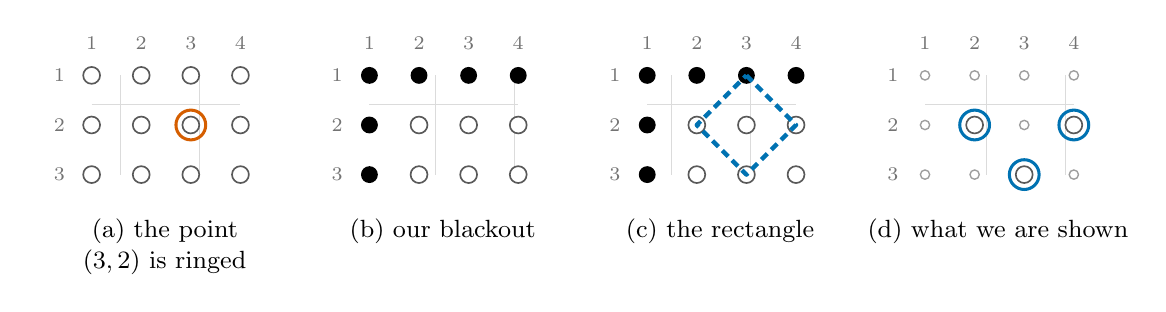
\begin{tikzpicture}[x=0.630cm,y=0.630cm,baseline=(current bounding box.north)]
  \draw[gridcol] (1,-1) grid (4,-3);
  \filldraw[fill=white,draw=keptline,line width=0.6pt] (1,-1) circle (0.17);
  \filldraw[fill=white,draw=keptline,line width=0.6pt] (2,-1) circle (0.17);
  \filldraw[fill=white,draw=keptline,line width=0.6pt] (3,-1) circle (0.17);
  \filldraw[fill=white,draw=keptline,line width=0.6pt] (4,-1) circle (0.17);
  \filldraw[fill=white,draw=keptline,line width=0.6pt] (1,-2) circle (0.17);
  \filldraw[fill=white,draw=keptline,line width=0.6pt] (2,-2) circle (0.17);
  \filldraw[fill=white,draw=keptline,line width=0.6pt] (3,-2) circle (0.17);
  \filldraw[fill=white,draw=keptline,line width=0.6pt] (4,-2) circle (0.17);
  \filldraw[fill=white,draw=keptline,line width=0.6pt] (1,-3) circle (0.17);
  \filldraw[fill=white,draw=keptline,line width=0.6pt] (2,-3) circle (0.17);
  \filldraw[fill=white,draw=keptline,line width=0.6pt] (3,-3) circle (0.17);
  \filldraw[fill=white,draw=keptline,line width=0.6pt] (4,-3) circle (0.17);
  \node[lab] at (1,-0.35) {1};
  \node[lab] at (2,-0.35) {2};
  \node[lab] at (3,-0.35) {3};
  \node[lab] at (4,-0.35) {4};
  \node[lab] at (0.35,-1) {1};
  \node[lab] at (0.35,-2) {2};
  \node[lab] at (0.35,-3) {3};
  \draw[rectB,line width=1.1pt] (3,-2) circle (0.3);
  \node[capt,anchor=north,text width=3.28cm,align=center] at (2.5,-3.7) {(a) the point $(3,2)$ is ringed};
  \draw[gridcol] (6.6,-1) grid (9.6,-3);
  \fill[black] (6.6,-1) circle (0.17);
  \fill[black] (7.6,-1) circle (0.17);
  \fill[black] (8.6,-1) circle (0.17);
  \fill[black] (9.6,-1) circle (0.17);
  \fill[black] (6.6,-2) circle (0.17);
  \filldraw[fill=white,draw=keptline,line width=0.6pt] (7.6,-2) circle (0.17);
  \filldraw[fill=white,draw=keptline,line width=0.6pt] (8.6,-2) circle (0.17);
  \filldraw[fill=white,draw=keptline,line width=0.6pt] (9.6,-2) circle (0.17);
  \fill[black] (6.6,-3) circle (0.17);
  \filldraw[fill=white,draw=keptline,line width=0.6pt] (7.6,-3) circle (0.17);
  \filldraw[fill=white,draw=keptline,line width=0.6pt] (8.6,-3) circle (0.17);
  \filldraw[fill=white,draw=keptline,line width=0.6pt] (9.6,-3) circle (0.17);
  \node[lab] at (6.6,-0.35) {1};
  \node[lab] at (7.6,-0.35) {2};
  \node[lab] at (8.6,-0.35) {3};
  \node[lab] at (9.6,-0.35) {4};
  \node[lab] at (5.949999999999999,-1) {1};
  \node[lab] at (5.949999999999999,-2) {2};
  \node[lab] at (5.949999999999999,-3) {3};
  \node[capt,anchor=north,text width=3.28cm,align=center] at (8.1,-3.7) {(b) our blackout};
  \draw[gridcol] (12.2,-1) grid (15.2,-3);
  \fill[black] (12.2,-1) circle (0.17);
  \fill[black] (13.2,-1) circle (0.17);
  \fill[black] (14.2,-1) circle (0.17);
  \fill[black] (15.2,-1) circle (0.17);
  \fill[black] (12.2,-2) circle (0.17);
  \filldraw[fill=white,draw=keptline,line width=0.6pt] (13.2,-2) circle (0.17);
  \filldraw[fill=white,draw=keptline,line width=0.6pt] (14.2,-2) circle (0.17);
  \filldraw[fill=white,draw=keptline,line width=0.6pt] (15.2,-2) circle (0.17);
  \fill[black] (12.2,-3) circle (0.17);
  \filldraw[fill=white,draw=keptline,line width=0.6pt] (13.2,-3) circle (0.17);
  \filldraw[fill=white,draw=keptline,line width=0.6pt] (14.2,-3) circle (0.17);
  \filldraw[fill=white,draw=keptline,line width=0.6pt] (15.2,-3) circle (0.17);
  \node[lab] at (12.2,-0.35) {1};
  \node[lab] at (13.2,-0.35) {2};
  \node[lab] at (14.2,-0.35) {3};
  \node[lab] at (15.2,-0.35) {4};
  \node[lab] at (11.549999999999999,-1) {1};
  \node[lab] at (11.549999999999999,-2) {2};
  \node[lab] at (11.549999999999999,-3) {3};
  \draw[draw=rectA,line width=1.6pt,line join=round,dash pattern=on 3pt off 2pt] (14.2,-1) -- (15.2,-2) -- (14.2,-3) -- (13.2,-2) -- cycle;
  \node[capt,anchor=north,text width=3.28cm,align=center] at (13.7,-3.7) {(c) the rectangle};
  \draw[gridcol] (17.799999999999997,-1) grid (20.799999999999997,-3);
  \draw[hidcol,line width=0.5pt] (17.799999999999997,-1) circle (0.09350000000000001);
  \draw[hidcol,line width=0.5pt] (18.799999999999997,-1) circle (0.09350000000000001);
  \draw[hidcol,line width=0.5pt] (19.799999999999997,-1) circle (0.09350000000000001);
  \draw[hidcol,line width=0.5pt] (20.799999999999997,-1) circle (0.09350000000000001);
  \draw[hidcol,line width=0.5pt] (17.799999999999997,-2) circle (0.09350000000000001);
  \filldraw[fill=white,draw=keptline,line width=0.6pt] (18.799999999999997,-2) circle (0.17);
  \draw[hidcol,line width=0.5pt] (19.799999999999997,-2) circle (0.09350000000000001);
  \filldraw[fill=white,draw=keptline,line width=0.6pt] (20.799999999999997,-2) circle (0.17);
  \draw[hidcol,line width=0.5pt] (17.799999999999997,-3) circle (0.09350000000000001);
  \draw[hidcol,line width=0.5pt] (18.799999999999997,-3) circle (0.09350000000000001);
  \filldraw[fill=white,draw=keptline,line width=0.6pt] (19.799999999999997,-3) circle (0.17);
  \draw[hidcol,line width=0.5pt] (20.799999999999997,-3) circle (0.09350000000000001);
  \node[lab] at (17.799999999999997,-0.35) {1};
  \node[lab] at (18.799999999999997,-0.35) {2};
  \node[lab] at (19.799999999999997,-0.35) {3};
  \node[lab] at (20.799999999999997,-0.35) {4};
  \node[lab] at (17.15,-1) {1};
  \node[lab] at (17.15,-2) {2};
  \node[lab] at (17.15,-3) {3};
  \draw[rectA,line width=1.1pt] (18.799999999999997,-2) circle (0.3);
  \draw[rectA,line width=1.1pt] (20.799999999999997,-2) circle (0.3);
  \draw[rectA,line width=1.1pt] (19.799999999999997,-3) circle (0.3);
  \node[capt,anchor=north,text width=3.28cm,align=center] at (19.299999999999997,-3.7) {(d) what we are shown};
\end{tikzpicture}

\caption{One round on the $3\times4$ grid. Black dots are blacked out and open dots are white.
In (d) the grey specks are points we are told nothing about.}
\label{fig:game}
\end{figure}

\begin{example}\label{ex:game}
Figure~\ref{fig:game} plays one round. In (b) we black out all of row 1 and all of column 1,
which is 6 points. In (c) the game master draws the tilted square with corners $(2,2)$, $(3,1)$,
$(4,2)$ and $(3,3)$. The corner $(3,1)$ is in row 1, so it is black, and in (d) we are only shown
$(2,2)$, $(4,2)$ and $(3,3)$. That is enough. Three corners of a rectangle always determine the
fourth (Lemma~\ref{lem:threecorners} below), and here the fourth corner has to be $(3,1)$. We
will see in Section~\ref{sec:three} that this blackout works against every rectangle on the
$3\times4$ grid, and that 6 is the most anyone can black out there.
\end{example}

\subsection{Conventions}\label{sec:conventions}

We use these conventions all the way through.
\begin{enumerate}[leftmargin=*,itemsep=1pt]
\item An $n\times m$ grid has $n$ rows and $m$ columns, so $nm$ points. A $2\times m$ grid is
called a \emph{strip}.
\item The point $(i,j)$ is in column $i$ and row $j$, and $(1,1)$ is the top-left point. So $i$
grows to the right and $j$ grows downwards, as in Figure~\ref{fig:game}(a). The set of all
points is $V$.
\item A \emph{rectangle} is any rectangle whose 4 corners are grid points, tilted ones included.
It must have positive area. We write $C(R)$ for the set of corners of $R$. Two different
rectangles have different corner sets, so we can think of a rectangle as its set of 4 corners.
\item A \emph{blackout} is a set $S\subseteq V$, and the \emph{kept set} is $K=V\setminus S$,
the points left white.
\end{enumerate}

How do we tell whether 4 points form a rectangle? Pair them up into 2 ``diagonals''. The 4
points form a parallelogram exactly when the 2 diagonals have the same midpoint, and the
parallelogram is a rectangle exactly when the 2 diagonals also have the same length. So 4
points are a rectangle if and only if some pairing gives 2 segments with the same midpoint and
the same length. The verification script finds all rectangles this way: it sorts all pairs of
points by midpoint and length and takes 2 pairs from the same class.

\begin{figure}[htbp]
\centering
% generated by make_figures.py; width about 12.8 cm
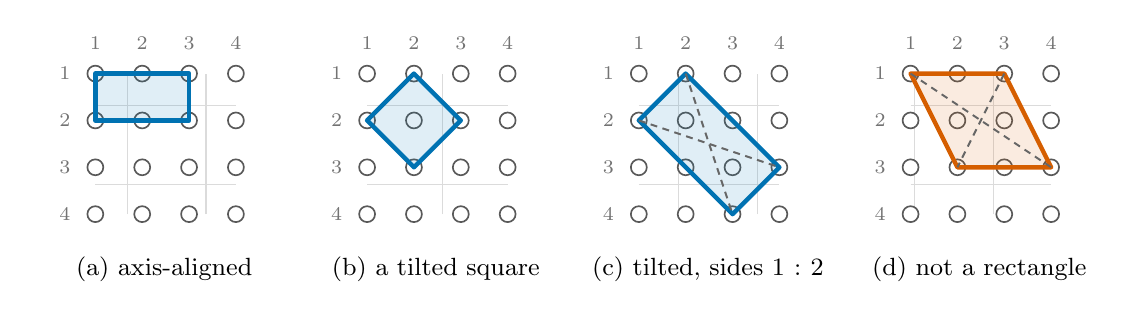
\begin{tikzpicture}[x=0.595cm,y=0.595cm,baseline=(current bounding box.north)]
  \draw[gridcol] (1.0,-1) grid (4.0,-4);
  \filldraw[fill=white,draw=keptline,line width=0.6pt] (1.0,-1) circle (0.17);
  \filldraw[fill=white,draw=keptline,line width=0.6pt] (2.0,-1) circle (0.17);
  \filldraw[fill=white,draw=keptline,line width=0.6pt] (3.0,-1) circle (0.17);
  \filldraw[fill=white,draw=keptline,line width=0.6pt] (4.0,-1) circle (0.17);
  \filldraw[fill=white,draw=keptline,line width=0.6pt] (1.0,-2) circle (0.17);
  \filldraw[fill=white,draw=keptline,line width=0.6pt] (2.0,-2) circle (0.17);
  \filldraw[fill=white,draw=keptline,line width=0.6pt] (3.0,-2) circle (0.17);
  \filldraw[fill=white,draw=keptline,line width=0.6pt] (4.0,-2) circle (0.17);
  \filldraw[fill=white,draw=keptline,line width=0.6pt] (1.0,-3) circle (0.17);
  \filldraw[fill=white,draw=keptline,line width=0.6pt] (2.0,-3) circle (0.17);
  \filldraw[fill=white,draw=keptline,line width=0.6pt] (3.0,-3) circle (0.17);
  \filldraw[fill=white,draw=keptline,line width=0.6pt] (4.0,-3) circle (0.17);
  \filldraw[fill=white,draw=keptline,line width=0.6pt] (1.0,-4) circle (0.17);
  \filldraw[fill=white,draw=keptline,line width=0.6pt] (2.0,-4) circle (0.17);
  \filldraw[fill=white,draw=keptline,line width=0.6pt] (3.0,-4) circle (0.17);
  \filldraw[fill=white,draw=keptline,line width=0.6pt] (4.0,-4) circle (0.17);
  \node[lab] at (1.0,-0.35) {1};
  \node[lab] at (2.0,-0.35) {2};
  \node[lab] at (3.0,-0.35) {3};
  \node[lab] at (4.0,-0.35) {4};
  \node[lab] at (0.35,-1) {1};
  \node[lab] at (0.35,-2) {2};
  \node[lab] at (0.35,-3) {3};
  \node[lab] at (0.35,-4) {4};
  \fill[rectA,opacity=0.12] (1.0,-1) -- (3.0,-1) -- (3.0,-2) -- (1.0,-2) -- cycle;
  \draw[draw=rectA,line width=1.6pt,line join=round] (1.0,-1) -- (3.0,-1) -- (3.0,-2) -- (1.0,-2) -- cycle;
  \node[capt,anchor=north,text width=3.27cm,align=center] at (2.5,-4.7) {(a) axis-aligned};
  \draw[gridcol] (6.8,-1) grid (9.8,-4);
  \filldraw[fill=white,draw=keptline,line width=0.6pt] (6.8,-1) circle (0.17);
  \filldraw[fill=white,draw=keptline,line width=0.6pt] (7.8,-1) circle (0.17);
  \filldraw[fill=white,draw=keptline,line width=0.6pt] (8.8,-1) circle (0.17);
  \filldraw[fill=white,draw=keptline,line width=0.6pt] (9.8,-1) circle (0.17);
  \filldraw[fill=white,draw=keptline,line width=0.6pt] (6.8,-2) circle (0.17);
  \filldraw[fill=white,draw=keptline,line width=0.6pt] (7.8,-2) circle (0.17);
  \filldraw[fill=white,draw=keptline,line width=0.6pt] (8.8,-2) circle (0.17);
  \filldraw[fill=white,draw=keptline,line width=0.6pt] (9.8,-2) circle (0.17);
  \filldraw[fill=white,draw=keptline,line width=0.6pt] (6.8,-3) circle (0.17);
  \filldraw[fill=white,draw=keptline,line width=0.6pt] (7.8,-3) circle (0.17);
  \filldraw[fill=white,draw=keptline,line width=0.6pt] (8.8,-3) circle (0.17);
  \filldraw[fill=white,draw=keptline,line width=0.6pt] (9.8,-3) circle (0.17);
  \filldraw[fill=white,draw=keptline,line width=0.6pt] (6.8,-4) circle (0.17);
  \filldraw[fill=white,draw=keptline,line width=0.6pt] (7.8,-4) circle (0.17);
  \filldraw[fill=white,draw=keptline,line width=0.6pt] (8.8,-4) circle (0.17);
  \filldraw[fill=white,draw=keptline,line width=0.6pt] (9.8,-4) circle (0.17);
  \node[lab] at (6.8,-0.35) {1};
  \node[lab] at (7.8,-0.35) {2};
  \node[lab] at (8.8,-0.35) {3};
  \node[lab] at (9.8,-0.35) {4};
  \node[lab] at (6.1499999999999995,-1) {1};
  \node[lab] at (6.1499999999999995,-2) {2};
  \node[lab] at (6.1499999999999995,-3) {3};
  \node[lab] at (6.1499999999999995,-4) {4};
  \fill[rectA,opacity=0.12] (7.8,-1) -- (8.8,-2) -- (7.8,-3) -- (6.8,-2) -- cycle;
  \draw[draw=rectA,line width=1.6pt,line join=round] (7.8,-1) -- (8.8,-2) -- (7.8,-3) -- (6.8,-2) -- cycle;
  \node[capt,anchor=north,text width=3.27cm,align=center] at (8.3,-4.7) {(b) a tilted square};
  \draw[gridcol] (12.6,-1) grid (15.6,-4);
  \filldraw[fill=white,draw=keptline,line width=0.6pt] (12.6,-1) circle (0.17);
  \filldraw[fill=white,draw=keptline,line width=0.6pt] (13.6,-1) circle (0.17);
  \filldraw[fill=white,draw=keptline,line width=0.6pt] (14.6,-1) circle (0.17);
  \filldraw[fill=white,draw=keptline,line width=0.6pt] (15.6,-1) circle (0.17);
  \filldraw[fill=white,draw=keptline,line width=0.6pt] (12.6,-2) circle (0.17);
  \filldraw[fill=white,draw=keptline,line width=0.6pt] (13.6,-2) circle (0.17);
  \filldraw[fill=white,draw=keptline,line width=0.6pt] (14.6,-2) circle (0.17);
  \filldraw[fill=white,draw=keptline,line width=0.6pt] (15.6,-2) circle (0.17);
  \filldraw[fill=white,draw=keptline,line width=0.6pt] (12.6,-3) circle (0.17);
  \filldraw[fill=white,draw=keptline,line width=0.6pt] (13.6,-3) circle (0.17);
  \filldraw[fill=white,draw=keptline,line width=0.6pt] (14.6,-3) circle (0.17);
  \filldraw[fill=white,draw=keptline,line width=0.6pt] (15.6,-3) circle (0.17);
  \filldraw[fill=white,draw=keptline,line width=0.6pt] (12.6,-4) circle (0.17);
  \filldraw[fill=white,draw=keptline,line width=0.6pt] (13.6,-4) circle (0.17);
  \filldraw[fill=white,draw=keptline,line width=0.6pt] (14.6,-4) circle (0.17);
  \filldraw[fill=white,draw=keptline,line width=0.6pt] (15.6,-4) circle (0.17);
  \node[lab] at (12.6,-0.35) {1};
  \node[lab] at (13.6,-0.35) {2};
  \node[lab] at (14.6,-0.35) {3};
  \node[lab] at (15.6,-0.35) {4};
  \node[lab] at (11.95,-1) {1};
  \node[lab] at (11.95,-2) {2};
  \node[lab] at (11.95,-3) {3};
  \node[lab] at (11.95,-4) {4};
  \fill[rectA,opacity=0.12] (12.6,-2) -- (13.6,-1) -- (15.6,-3) -- (14.6,-4) -- cycle;
  \draw[draw=rectA,line width=1.6pt,line join=round] (12.6,-2) -- (13.6,-1) -- (15.6,-3) -- (14.6,-4) -- cycle;
  \draw[draw=black!60,line width=0.7pt,dash pattern=on 2.5pt off 2pt] (12.6,-2) -- (15.6,-3);
  \draw[draw=black!60,line width=0.7pt,dash pattern=on 2.5pt off 2pt] (13.6,-1) -- (14.6,-4);
  \node[capt,anchor=north,text width=3.27cm,align=center] at (14.1,-4.7) {(c) tilted, sides $1:2$};
  \draw[gridcol] (18.4,-1) grid (21.4,-4);
  \filldraw[fill=white,draw=keptline,line width=0.6pt] (18.4,-1) circle (0.17);
  \filldraw[fill=white,draw=keptline,line width=0.6pt] (19.4,-1) circle (0.17);
  \filldraw[fill=white,draw=keptline,line width=0.6pt] (20.4,-1) circle (0.17);
  \filldraw[fill=white,draw=keptline,line width=0.6pt] (21.4,-1) circle (0.17);
  \filldraw[fill=white,draw=keptline,line width=0.6pt] (18.4,-2) circle (0.17);
  \filldraw[fill=white,draw=keptline,line width=0.6pt] (19.4,-2) circle (0.17);
  \filldraw[fill=white,draw=keptline,line width=0.6pt] (20.4,-2) circle (0.17);
  \filldraw[fill=white,draw=keptline,line width=0.6pt] (21.4,-2) circle (0.17);
  \filldraw[fill=white,draw=keptline,line width=0.6pt] (18.4,-3) circle (0.17);
  \filldraw[fill=white,draw=keptline,line width=0.6pt] (19.4,-3) circle (0.17);
  \filldraw[fill=white,draw=keptline,line width=0.6pt] (20.4,-3) circle (0.17);
  \filldraw[fill=white,draw=keptline,line width=0.6pt] (21.4,-3) circle (0.17);
  \filldraw[fill=white,draw=keptline,line width=0.6pt] (18.4,-4) circle (0.17);
  \filldraw[fill=white,draw=keptline,line width=0.6pt] (19.4,-4) circle (0.17);
  \filldraw[fill=white,draw=keptline,line width=0.6pt] (20.4,-4) circle (0.17);
  \filldraw[fill=white,draw=keptline,line width=0.6pt] (21.4,-4) circle (0.17);
  \node[lab] at (18.4,-0.35) {1};
  \node[lab] at (19.4,-0.35) {2};
  \node[lab] at (20.4,-0.35) {3};
  \node[lab] at (21.4,-0.35) {4};
  \node[lab] at (17.75,-1) {1};
  \node[lab] at (17.75,-2) {2};
  \node[lab] at (17.75,-3) {3};
  \node[lab] at (17.75,-4) {4};
  \fill[rectB,opacity=0.12] (18.4,-1) -- (20.4,-1) -- (21.4,-3) -- (19.4,-3) -- cycle;
  \draw[draw=rectB,line width=1.6pt,line join=round] (18.4,-1) -- (20.4,-1) -- (21.4,-3) -- (19.4,-3) -- cycle;
  \draw[draw=black!60,line width=0.7pt,dash pattern=on 2.5pt off 2pt] (18.4,-1) -- (21.4,-3);
  \draw[draw=black!60,line width=0.7pt,dash pattern=on 2.5pt off 2pt] (20.4,-1) -- (19.4,-3);
  \node[capt,anchor=north,text width=3.27cm,align=center] at (19.9,-4.7) {(d) not a rectangle};
\end{tikzpicture}

\caption{Which 4-point sets are rectangles, on the $4\times4$ grid. In (c) and (d) the dashed
lines are the diagonals.}
\label{fig:rects}
\end{figure}

\begin{example}
In Figure~\ref{fig:rects}(c) the diagonals join $(1,2)$ to $(4,3)$ and $(2,1)$ to $(3,4)$.
Both have midpoint $(\frac52,\frac52)$, and both have squared length $3^2+1^2=1^2+3^2=10$, so
the 4 points are a rectangle, with sides of length $\sqrt2$ and $2\sqrt2$. In (d) the diagonals
join $(1,1)$ to $(4,3)$ and $(3,1)$ to $(2,3)$. They have the same midpoint $(\frac52,2)$, so
the shape is a parallelogram, but the squared lengths are $13$ and $5$, so it is not a rectangle.
\end{example}

The number of rectangles grows quickly. The $3\times3$ grid has 10 (9 axis-aligned and 1 tilted
square), the $4\times4$ grid has 44 (36 and 8), and the $5\times5$ grid has 130 (100 and 30).
The counts on square grids, $1,10,44,130,313,\ldots$, are OEIS A085582 \cite{oeisA085582}, and
the counts on $n\times m$ grids are in OEIS A289832 \cite{oeisA289832}. Our counts agree with
both everywhere we computed them.

\subsection{What the player sees}

For a blackout $S$ and a rectangle $R$, what we are shown is the set of white corners,
\[
\pres(R)=C(R)\setminus S .
\]
We call $\pres(R)$ the \emph{presentation} of $R$.

\begin{definition}
A blackout $S$ is \emph{valid} if different rectangles always have different presentations,
that is, if $\pres(R_1)\ne\pres(R_2)$ whenever $R_1\ne R_2$. The \emph{maximum blackout} of a
grid is the largest size of a valid blackout.
\end{definition}

The empty set is allowed as a presentation. It just means every corner was black. We don't need
a separate rule about it.

\begin{remark}\label{rem:empty}
Suppose 2 distinct rectangles $R_1\ne R_2$ are both fully hidden, that is,
$C(R_1)\subseteq S$ and $C(R_2)\subseteq S$. Then $\pres(R_1)=\emptyset=\pres(R_2)$, so $S$ is
not valid. Hence at most 1 rectangle can be fully hidden under a valid blackout. This follows
from the definition; it isn't an extra rule.
\end{remark}

\subsection{A first example: the $2\times3$ strip}

On 2 rows every rectangle is axis-aligned, because a tilted rectangle has its 4 corners in at
least 3 different rows. An axis-aligned rectangle on a strip uses both rows and 2 columns
$a<b$, and we call it $R_{a,b}$. The $2\times3$ strip has the 3 rectangles of
Figure~\ref{fig:striprects}.

\begin{figure}[htbp]
\centering
% generated by make_figures.py; width about 9.2 cm
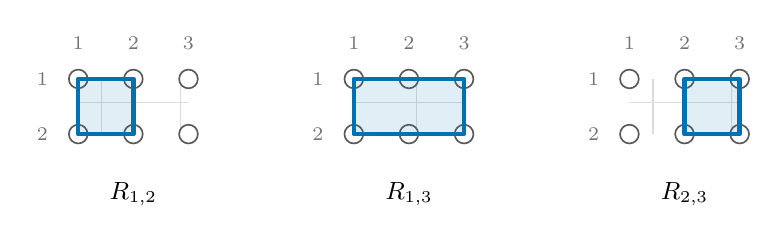
\begin{tikzpicture}[x=0.700cm,y=0.700cm,baseline=(current bounding box.north)]
  \draw[gridcol] (1.0,-1) grid (3.0,-2);
  \filldraw[fill=white,draw=keptline,line width=0.6pt] (1.0,-1) circle (0.17);
  \filldraw[fill=white,draw=keptline,line width=0.6pt] (2.0,-1) circle (0.17);
  \filldraw[fill=white,draw=keptline,line width=0.6pt] (3.0,-1) circle (0.17);
  \filldraw[fill=white,draw=keptline,line width=0.6pt] (1.0,-2) circle (0.17);
  \filldraw[fill=white,draw=keptline,line width=0.6pt] (2.0,-2) circle (0.17);
  \filldraw[fill=white,draw=keptline,line width=0.6pt] (3.0,-2) circle (0.17);
  \node[lab] at (1.0,-0.35) {1};
  \node[lab] at (2.0,-0.35) {2};
  \node[lab] at (3.0,-0.35) {3};
  \node[lab] at (0.35,-1) {1};
  \node[lab] at (0.35,-2) {2};
  \fill[rectA,opacity=0.12] (1.0,-1) -- (2.0,-1) -- (2.0,-2) -- (1.0,-2) -- cycle;
  \draw[draw=rectA,line width=1.6pt,line join=round] (1.0,-1) -- (2.0,-1) -- (2.0,-2) -- (1.0,-2) -- cycle;
  \node[capt,anchor=north] at (2.0,-2.7) {$R_{1,2}$};
  \draw[gridcol] (6.0,-1) grid (8.0,-2);
  \filldraw[fill=white,draw=keptline,line width=0.6pt] (6.0,-1) circle (0.17);
  \filldraw[fill=white,draw=keptline,line width=0.6pt] (7.0,-1) circle (0.17);
  \filldraw[fill=white,draw=keptline,line width=0.6pt] (8.0,-1) circle (0.17);
  \filldraw[fill=white,draw=keptline,line width=0.6pt] (6.0,-2) circle (0.17);
  \filldraw[fill=white,draw=keptline,line width=0.6pt] (7.0,-2) circle (0.17);
  \filldraw[fill=white,draw=keptline,line width=0.6pt] (8.0,-2) circle (0.17);
  \node[lab] at (6.0,-0.35) {1};
  \node[lab] at (7.0,-0.35) {2};
  \node[lab] at (8.0,-0.35) {3};
  \node[lab] at (5.35,-1) {1};
  \node[lab] at (5.35,-2) {2};
  \fill[rectA,opacity=0.12] (6.0,-1) -- (8.0,-1) -- (8.0,-2) -- (6.0,-2) -- cycle;
  \draw[draw=rectA,line width=1.6pt,line join=round] (6.0,-1) -- (8.0,-1) -- (8.0,-2) -- (6.0,-2) -- cycle;
  \node[capt,anchor=north] at (7.0,-2.7) {$R_{1,3}$};
  \draw[gridcol] (11.0,-1) grid (13.0,-2);
  \filldraw[fill=white,draw=keptline,line width=0.6pt] (11.0,-1) circle (0.17);
  \filldraw[fill=white,draw=keptline,line width=0.6pt] (12.0,-1) circle (0.17);
  \filldraw[fill=white,draw=keptline,line width=0.6pt] (13.0,-1) circle (0.17);
  \filldraw[fill=white,draw=keptline,line width=0.6pt] (11.0,-2) circle (0.17);
  \filldraw[fill=white,draw=keptline,line width=0.6pt] (12.0,-2) circle (0.17);
  \filldraw[fill=white,draw=keptline,line width=0.6pt] (13.0,-2) circle (0.17);
  \node[lab] at (11.0,-0.35) {1};
  \node[lab] at (12.0,-0.35) {2};
  \node[lab] at (13.0,-0.35) {3};
  \node[lab] at (10.35,-1) {1};
  \node[lab] at (10.35,-2) {2};
  \fill[rectA,opacity=0.12] (12.0,-1) -- (13.0,-1) -- (13.0,-2) -- (12.0,-2) -- cycle;
  \draw[draw=rectA,line width=1.6pt,line join=round] (12.0,-1) -- (13.0,-1) -- (13.0,-2) -- (12.0,-2) -- cycle;
  \node[capt,anchor=north] at (12.0,-2.7) {$R_{2,3}$};
\end{tikzpicture}

\caption{The 3 rectangles of the $2\times3$ strip.}
\label{fig:striprects}
\end{figure}

\begin{figure}[htbp]
\centering
% generated by make_figures.py; width about 6.8 cm
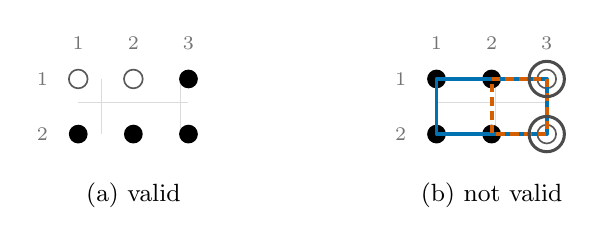
\begin{tikzpicture}[x=0.700cm,y=0.700cm,baseline=(current bounding box.north)]
  \draw[gridcol] (1,-1) grid (3,-2);
  \filldraw[fill=white,draw=keptline,line width=0.6pt] (1,-1) circle (0.17);
  \filldraw[fill=white,draw=keptline,line width=0.6pt] (2,-1) circle (0.17);
  \fill[black] (3,-1) circle (0.17);
  \fill[black] (1,-2) circle (0.17);
  \fill[black] (2,-2) circle (0.17);
  \fill[black] (3,-2) circle (0.17);
  \node[lab] at (1,-0.35) {1};
  \node[lab] at (2,-0.35) {2};
  \node[lab] at (3,-0.35) {3};
  \node[lab] at (0.35,-1) {1};
  \node[lab] at (0.35,-2) {2};
  \node[capt,anchor=north] at (2,-2.7) {(a) valid};
  \draw[gridcol] (7.5,-1) grid (9.5,-2);
  \fill[black] (7.5,-1) circle (0.17);
  \fill[black] (8.5,-1) circle (0.17);
  \filldraw[fill=white,draw=keptline,line width=0.6pt] (9.5,-1) circle (0.17);
  \fill[black] (7.5,-2) circle (0.17);
  \fill[black] (8.5,-2) circle (0.17);
  \filldraw[fill=white,draw=keptline,line width=0.6pt] (9.5,-2) circle (0.17);
  \node[lab] at (7.5,-0.35) {1};
  \node[lab] at (8.5,-0.35) {2};
  \node[lab] at (9.5,-0.35) {3};
  \node[lab] at (6.85,-1) {1};
  \node[lab] at (6.85,-2) {2};
  \draw[draw=rectA,line width=1.4pt,line join=round] (7.5,-1) -- (9.5,-1) -- (9.5,-2) -- (7.5,-2) -- cycle;
  \draw[draw=rectB,line width=1.4pt,line join=round,dash pattern=on 3pt off 2pt] (8.5,-1) -- (9.5,-1) -- (9.5,-2) -- (8.5,-2) -- cycle;
  \draw[black!70,line width=1.1pt] (9.5,-1) circle (0.32);
  \draw[black!70,line width=1.1pt] (9.5,-2) circle (0.32);
  \node[capt,anchor=north] at (8.5,-2.7) {(b) not valid};
\end{tikzpicture}

\caption{Two blackouts of 4 points on the $2\times3$ strip. In (b) the rectangles $R_{1,3}$
(solid) and $R_{2,3}$ (dashed) both show exactly the ringed points.}
\label{fig:twoblackouts}
\end{figure}

\begin{example}\label{ex:2x3}
Figure~\ref{fig:twoblackouts} shows 2 blackouts with 4 points each. Here are the presentations:
\begin{center}
\begin{tabular}{lll}
\toprule
rectangle & blackout (a) & blackout (b)\\
\midrule
$R_{1,2}$ & $\{(1,1),(2,1)\}$ & $\emptyset$ \\
$R_{1,3}$ & $\{(1,1)\}$ & $\{(3,1),(3,2)\}$ \\
$R_{2,3}$ & $\{(2,1)\}$ & $\{(3,1),(3,2)\}$ \\
\bottomrule
\end{tabular}
\end{center}
In (a) the 3 presentations are different, so (a) is valid. In (b) the rectangles $R_{1,3}$ and
$R_{2,3}$ look the same. If we are shown $(3,1)$ and $(3,2)$ we can't tell whether the left side
is in column 1 or column 2, so (b) is not valid. Both blackouts have 4 points, so the size alone
doesn't decide anything; where the points go matters.

Can we black out 5 points? Then only 1 point is kept, and every presentation is either empty or
that 1 point. That is 2 possible presentations for 3 rectangles, so 2 of them must agree. So the
maximum blackout of the $2\times3$ strip is 4.
\end{example}

%======================================================================
\section{From the game to a hitting set}\label{sec:reduction}

\subsection{When do 2 rectangles look the same?}

\begin{lemma}[difference sets]\label{lem:reduction}
For any sets $A,B,S$: \ $A\setminus S=B\setminus S$ if and only if $A\,\triangle\,B\subseteq S$.
\end{lemma}

Here $A\triangle B=(A\setminus B)\cup(B\setminus A)$ is the set of points in exactly 1 of $A$ and
$B$. In words: 2 rectangles look the same exactly when every corner that belongs to only 1 of
them is black. The corners they share don't matter, since they are shown or hidden for both.

\begin{proof}
($\Rightarrow$) Assume $A\setminus S=B\setminus S$, and let $x\in A\,\triangle\,B$ be arbitrary.
The statement is symmetric in $A$ and $B$, so we may assume $x\in A\setminus B$. Suppose
$x\notin S$. Then $x\in A\setminus S=B\setminus S$, so $x\in B$, which contradicts
$x\in A\setminus B$. Therefore $x\in S$. As $x$ was arbitrary, $A\,\triangle\,B\subseteq S$.

($\Leftarrow$) Assume $A\,\triangle\,B\subseteq S$. By symmetry it is enough to prove
$A\setminus S\subseteq B\setminus S$. Let $x\in A\setminus S$ be arbitrary, so $x\in A$ and
$x\notin S$. Suppose $x\notin B$. Then $x\in A\setminus B\subseteq A\,\triangle\,B\subseteq S$,
which contradicts $x\notin S$. Hence $x\in B$, and with $x\notin S$ we get $x\in B\setminus S$.
\end{proof}

\begin{figure}[htbp]
\centering
% generated by make_figures.py; width about 7.8 cm
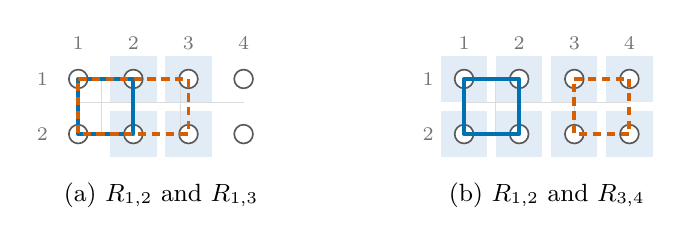
\begin{tikzpicture}[x=0.700cm,y=0.700cm,baseline=(current bounding box.north)]
  \fill[keptcol] (1.58,-1.42) rectangle (2.42,-0.5800000000000001);
  \fill[keptcol] (1.58,-2.42) rectangle (2.42,-1.58);
  \fill[keptcol] (2.58,-1.42) rectangle (3.42,-0.5800000000000001);
  \fill[keptcol] (2.58,-2.42) rectangle (3.42,-1.58);
  \draw[gridcol] (1,-1) grid (4,-2);
  \filldraw[fill=white,draw=keptline,line width=0.6pt] (1,-1) circle (0.17);
  \filldraw[fill=white,draw=keptline,line width=0.6pt] (2,-1) circle (0.17);
  \filldraw[fill=white,draw=keptline,line width=0.6pt] (3,-1) circle (0.17);
  \filldraw[fill=white,draw=keptline,line width=0.6pt] (4,-1) circle (0.17);
  \filldraw[fill=white,draw=keptline,line width=0.6pt] (1,-2) circle (0.17);
  \filldraw[fill=white,draw=keptline,line width=0.6pt] (2,-2) circle (0.17);
  \filldraw[fill=white,draw=keptline,line width=0.6pt] (3,-2) circle (0.17);
  \filldraw[fill=white,draw=keptline,line width=0.6pt] (4,-2) circle (0.17);
  \node[lab] at (1,-0.35) {1};
  \node[lab] at (2,-0.35) {2};
  \node[lab] at (3,-0.35) {3};
  \node[lab] at (4,-0.35) {4};
  \node[lab] at (0.35,-1) {1};
  \node[lab] at (0.35,-2) {2};
  \draw[draw=rectA,line width=1.4pt,line join=round] (1,-1) -- (2,-1) -- (2,-2) -- (1,-2) -- cycle;
  \draw[draw=rectB,line width=1.4pt,line join=round,dash pattern=on 3pt off 2pt] (1,-1) -- (3,-1) -- (3,-2) -- (1,-2) -- cycle;
  \node[capt,anchor=north] at (2.5,-2.7) {(a) $R_{1,2}$ and $R_{1,3}$};
  \fill[keptcol] (7.58,-2.42) rectangle (8.42,-1.58);
  \fill[keptcol] (8.58,-1.42) rectangle (9.42,-0.5800000000000001);
  \fill[keptcol] (9.58,-1.42) rectangle (10.42,-0.5800000000000001);
  \fill[keptcol] (7.58,-1.42) rectangle (8.42,-0.5800000000000001);
  \fill[keptcol] (10.58,-2.42) rectangle (11.42,-1.58);
  \fill[keptcol] (8.58,-2.42) rectangle (9.42,-1.58);
  \fill[keptcol] (9.58,-2.42) rectangle (10.42,-1.58);
  \fill[keptcol] (10.58,-1.42) rectangle (11.42,-0.5800000000000001);
  \draw[gridcol] (8.0,-1) grid (11.0,-2);
  \filldraw[fill=white,draw=keptline,line width=0.6pt] (8.0,-1) circle (0.17);
  \filldraw[fill=white,draw=keptline,line width=0.6pt] (9.0,-1) circle (0.17);
  \filldraw[fill=white,draw=keptline,line width=0.6pt] (10.0,-1) circle (0.17);
  \filldraw[fill=white,draw=keptline,line width=0.6pt] (11.0,-1) circle (0.17);
  \filldraw[fill=white,draw=keptline,line width=0.6pt] (8.0,-2) circle (0.17);
  \filldraw[fill=white,draw=keptline,line width=0.6pt] (9.0,-2) circle (0.17);
  \filldraw[fill=white,draw=keptline,line width=0.6pt] (10.0,-2) circle (0.17);
  \filldraw[fill=white,draw=keptline,line width=0.6pt] (11.0,-2) circle (0.17);
  \node[lab] at (8.0,-0.35) {1};
  \node[lab] at (9.0,-0.35) {2};
  \node[lab] at (10.0,-0.35) {3};
  \node[lab] at (11.0,-0.35) {4};
  \node[lab] at (7.35,-1) {1};
  \node[lab] at (7.35,-2) {2};
  \draw[draw=rectA,line width=1.4pt,line join=round] (8.0,-1) -- (9.0,-1) -- (9.0,-2) -- (8.0,-2) -- cycle;
  \draw[draw=rectB,line width=1.4pt,line join=round,dash pattern=on 3pt off 2pt] (10.0,-1) -- (11.0,-1) -- (11.0,-2) -- (10.0,-2) -- cycle;
  \node[capt,anchor=north] at (9.5,-2.7) {(b) $R_{1,2}$ and $R_{3,4}$};
\end{tikzpicture}

\caption{Difference sets on the $2\times4$ strip. The shaded points are $C(R_1)\triangle
C(R_2)$ for the solid and the dashed rectangle.}
\label{fig:difference}
\end{figure}

\begin{example}
In Figure~\ref{fig:difference}(a), $R_{1,2}$ and $R_{1,3}$ share column 1. Their corners in
column 1 cancel, and the difference set is the 4 points of columns 2 and 3. By
Lemma~\ref{lem:reduction}, the 2 rectangles look the same exactly when all 4 shaded points are
black. To keep them apart we must keep at least 1 of those 4 points. In (b) the rectangles
$R_{1,2}$ and $R_{3,4}$ share nothing, and the difference set is all 8 points.
\end{example}

Applying the lemma to every pair of rectangles gives the following.

\begin{corollary}\label{cor:hitting}
A blackout $S$ is valid if and only if the kept set $K=V\setminus S$ contains at least 1 point
of $C(R_1)\triangle C(R_2)$ for every pair of distinct rectangles $R_1,R_2$.
\end{corollary}

\begin{proof}
$S$ is valid if and only if $C(R_1)\setminus S\ne C(R_2)\setminus S$ for every pair of distinct
rectangles. By Lemma~\ref{lem:reduction} this holds if and only if
$C(R_1)\triangle C(R_2)\not\subseteq S$ for every pair, which says exactly that some point of
the difference set lies in $K$.
\end{proof}

So the problem is really about the \emph{difference hypergraph}: the collection of all
difference sets $C(R_1)\triangle C(R_2)$. A set that meets every difference set is a
\emph{hitting set}, and
\[
\text{maximum blackout}=nm-\text{(smallest size of a hitting set)}.
\]
Small blackouts are easy; the work is in keeping very few points and still meeting every
difference set. The computer program in Section~\ref{sec:computations} solves exactly this
hitting set problem.

\subsection{Pruning}\label{sec:pruning}

Before computing anything we shrink the list of difference sets. Think of it as a table with one
line for each pair of rectangles. To avoid confusing these lines with rows of the grid, we call
them \emph{constraints}.

\begin{enumerate}[leftmargin=*,itemsep=1pt]
\item \emph{Repeats.} Two identical constraints say the same thing, so we keep 1 copy.
\item \emph{Containment.} If $D_1\subsetneq D_2$, any $K$ that meets $D_1$ also meets $D_2$, so
$D_2$ can be deleted without changing which kept sets are valid.
\item \emph{No empty constraints.} $C(R_1)\triangle C(R_2)=\emptyset$ would mean
$C(R_1)=C(R_2)$, and different rectangles have different corners, so this never happens.
\end{enumerate}

After pruning we are left with the minimal constraints, and a set $K$ meets every constraint if
and only if it meets every minimal one.

\begin{example}\label{ex:prune}
The $2\times4$ strip has 6 rectangles, so 15 pairs. Every rectangle is made of whole columns, so
each difference set is a set of whole columns too. Here is the full table, listing the columns
in each difference set.
\begin{center}\small
\begin{tabular}{llcl}
\toprule
pair & columns & points & after pruning\\
\midrule
$R_{1,2}$, $R_{1,3}$ & $\{2,3\}$ & 4 & kept \\
$R_{1,2}$, $R_{1,4}$ & $\{2,4\}$ & 4 & kept \\
$R_{1,2}$, $R_{2,3}$ & $\{1,3\}$ & 4 & kept \\
$R_{1,2}$, $R_{2,4}$ & $\{1,4\}$ & 4 & kept \\
$R_{1,2}$, $R_{3,4}$ & $\{1,2,3,4\}$ & 8 & deleted, contains columns $\{1,2\}$ \\
$R_{1,3}$, $R_{1,4}$ & $\{3,4\}$ & 4 & kept \\
$R_{1,3}$, $R_{2,3}$ & $\{1,2\}$ & 4 & kept \\
$R_{1,3}$, $R_{2,4}$ & $\{1,2,3,4\}$ & 8 & deleted, contains columns $\{1,2\}$ \\
$R_{1,3}$, $R_{3,4}$ & $\{1,4\}$ & 4 & repeat \\
$R_{1,4}$, $R_{2,3}$ & $\{1,2,3,4\}$ & 8 & deleted, contains columns $\{1,2\}$ \\
$R_{1,4}$, $R_{2,4}$ & $\{1,2\}$ & 4 & repeat \\
$R_{1,4}$, $R_{3,4}$ & $\{1,3\}$ & 4 & repeat \\
$R_{2,3}$, $R_{2,4}$ & $\{3,4\}$ & 4 & repeat \\
$R_{2,3}$, $R_{3,4}$ & $\{2,4\}$ & 4 & repeat \\
$R_{2,4}$, $R_{3,4}$ & $\{2,3\}$ & 4 & repeat \\
\bottomrule
\end{tabular}
\end{center}
Of the 15 lines, 6 survive, one for each pair of columns. So a kept set is valid on the
$2\times4$ strip if and only if, for every 2 columns, it keeps a point in at least 1 of them.
\end{example}

%======================================================================
\section{Two rows: the Strip Theorem}\label{sec:strip}

Example~\ref{ex:prune} already contains the whole idea for strips.

\begin{theorem}[Strip Theorem]\label{thm:strip}
Let $m\ge3$. The maximum blackout of the $2\times m$ strip is $m+1$. There are exactly
$m\cdot2^{m-1}$ maximum blackouts: black out both points of 1 column, and exactly 1 of the 2
points of every other column. For $m=2$ there is only 1 rectangle, so every blackout is valid
and the maximum is 4.
\end{theorem}

\begin{proof}
\emph{Step 1: the constraints.} Take 2 distinct rectangles $R_{a,b}$ and $R_{c,d}$. They can't
share both columns. If they share exactly 1 column, the shared column cancels and the difference
set is the 4 points of the other 2 columns $p,q$. We call this the \emph{pair constraint} on
$\{p,q\}$. If they share no column, the difference set is all 8 points of 4 columns, and it
contains a pair constraint, so pruning deletes it. Every pair $\{p,q\}$ does occur: since
$m\ge3$ there is a third column $z$, and $R_{z,p}$, $R_{z,q}$ (with the columns put in order)
have difference set exactly the pair constraint on $\{p,q\}$. So after pruning the constraints
are exactly the $\binom m2$ pair constraints.

\emph{Step 2: at most 1 empty column.} Let $K$ be a valid kept set and call a column empty if
$K$ has no point in it. If 2 columns $p\ne q$ were empty, $K$ would miss the pair constraint on
$\{p,q\}$. So at most 1 column is empty.

\emph{Step 3: the bound.} Every non-empty column has at least 1 kept point, so
$|K|\ge m-1$ and $|S|=2m-|K|\le m+1$. If equality holds then $|K|=m-1$ exactly, so exactly 1
column is empty (if none were, $|K|\ge m$) and every other column has exactly 1 kept point.

\emph{Step 4: these all work.} Take any $K$ with 1 empty column and exactly 1 point in every
other column. Any 2 columns include at least 1 non-empty one, whose kept point meets the pair
constraint. So $K$ is valid by Corollary~\ref{cor:hitting}, and $S=V\setminus K$ has $m+1$
points. There are $m$ choices for the empty column and 2 choices in each of the other $m-1$
columns, so $m\cdot2^{m-1}$ maximum blackouts.
\end{proof}

\begin{figure}[htbp]
\centering
% generated by make_figures.py; width about 4.3 cm
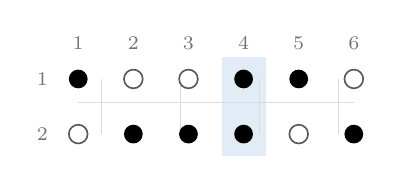
\begin{tikzpicture}[x=0.700cm,y=0.700cm,baseline=(current bounding box.north)]
  \fill[keptcol] (3.6,-0.6) rectangle (4.4,-2.4);
  \draw[gridcol] (1,-1) grid (6,-2);
  \fill[black] (1,-1) circle (0.17);
  \filldraw[fill=white,draw=keptline,line width=0.6pt] (2,-1) circle (0.17);
  \filldraw[fill=white,draw=keptline,line width=0.6pt] (3,-1) circle (0.17);
  \fill[black] (4,-1) circle (0.17);
  \fill[black] (5,-1) circle (0.17);
  \filldraw[fill=white,draw=keptline,line width=0.6pt] (6,-1) circle (0.17);
  \filldraw[fill=white,draw=keptline,line width=0.6pt] (1,-2) circle (0.17);
  \fill[black] (2,-2) circle (0.17);
  \fill[black] (3,-2) circle (0.17);
  \fill[black] (4,-2) circle (0.17);
  \filldraw[fill=white,draw=keptline,line width=0.6pt] (5,-2) circle (0.17);
  \fill[black] (6,-2) circle (0.17);
  \node[lab] at (1,-0.35) {1};
  \node[lab] at (2,-0.35) {2};
  \node[lab] at (3,-0.35) {3};
  \node[lab] at (4,-0.35) {4};
  \node[lab] at (5,-0.35) {5};
  \node[lab] at (6,-0.35) {6};
  \node[lab] at (0.35,-1) {1};
  \node[lab] at (0.35,-2) {2};
\end{tikzpicture}

\caption{A maximum blackout of the $2\times6$ strip: column 4 (shaded) is fully black and every
other column has 1 black point. It has $m+1=7$ points.}
\label{fig:stripmax}
\end{figure}

\begin{figure}[htbp]
\centering
% generated by make_figures.py; width about 15.2 cm
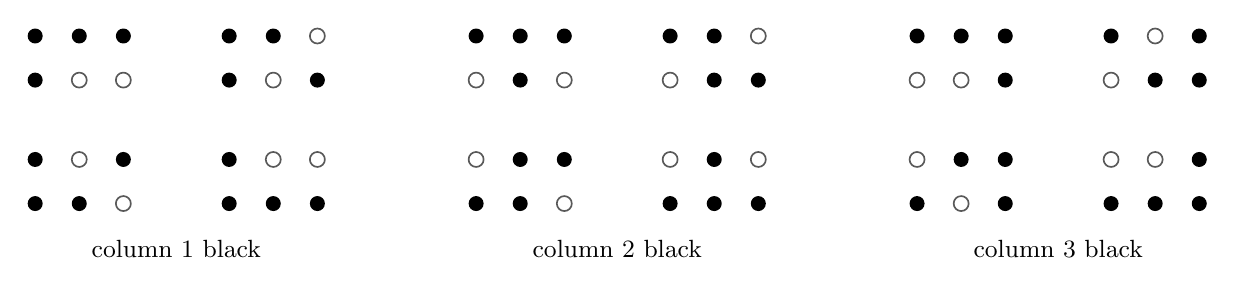
\begin{tikzpicture}[x=0.560cm,y=0.560cm,baseline=(current bounding box.north)]
  \begin{scope}[yshift=0.000cm]
  \fill[black] (1.0,-1) circle (0.17);
  \fill[black] (2.0,-1) circle (0.17);
  \fill[black] (3.0,-1) circle (0.17);
  \fill[black] (1.0,-2) circle (0.17);
  \filldraw[fill=white,draw=keptline,line width=0.6pt] (2.0,-2) circle (0.17);
  \filldraw[fill=white,draw=keptline,line width=0.6pt] (3.0,-2) circle (0.17);
  \end{scope}
  \begin{scope}[yshift=0.000cm]
  \fill[black] (5.4,-1) circle (0.17);
  \fill[black] (6.4,-1) circle (0.17);
  \filldraw[fill=white,draw=keptline,line width=0.6pt] (7.4,-1) circle (0.17);
  \fill[black] (5.4,-2) circle (0.17);
  \filldraw[fill=white,draw=keptline,line width=0.6pt] (6.4,-2) circle (0.17);
  \fill[black] (7.4,-2) circle (0.17);
  \end{scope}
  \begin{scope}[yshift=-1.568cm]
  \fill[black] (1.0,-1) circle (0.17);
  \filldraw[fill=white,draw=keptline,line width=0.6pt] (2.0,-1) circle (0.17);
  \fill[black] (3.0,-1) circle (0.17);
  \fill[black] (1.0,-2) circle (0.17);
  \fill[black] (2.0,-2) circle (0.17);
  \filldraw[fill=white,draw=keptline,line width=0.6pt] (3.0,-2) circle (0.17);
  \end{scope}
  \begin{scope}[yshift=-1.568cm]
  \fill[black] (5.4,-1) circle (0.17);
  \filldraw[fill=white,draw=keptline,line width=0.6pt] (6.4,-1) circle (0.17);
  \filldraw[fill=white,draw=keptline,line width=0.6pt] (7.4,-1) circle (0.17);
  \fill[black] (5.4,-2) circle (0.17);
  \fill[black] (6.4,-2) circle (0.17);
  \fill[black] (7.4,-2) circle (0.17);
  \end{scope}
  \node[capt,anchor=north] at (4.2,-5.4) {column 1 black};
  \begin{scope}[yshift=0.000cm]
  \fill[black] (11.0,-1) circle (0.17);
  \fill[black] (12.0,-1) circle (0.17);
  \fill[black] (13.0,-1) circle (0.17);
  \filldraw[fill=white,draw=keptline,line width=0.6pt] (11.0,-2) circle (0.17);
  \fill[black] (12.0,-2) circle (0.17);
  \filldraw[fill=white,draw=keptline,line width=0.6pt] (13.0,-2) circle (0.17);
  \end{scope}
  \begin{scope}[yshift=0.000cm]
  \fill[black] (15.4,-1) circle (0.17);
  \fill[black] (16.4,-1) circle (0.17);
  \filldraw[fill=white,draw=keptline,line width=0.6pt] (17.4,-1) circle (0.17);
  \filldraw[fill=white,draw=keptline,line width=0.6pt] (15.4,-2) circle (0.17);
  \fill[black] (16.4,-2) circle (0.17);
  \fill[black] (17.4,-2) circle (0.17);
  \end{scope}
  \begin{scope}[yshift=-1.568cm]
  \filldraw[fill=white,draw=keptline,line width=0.6pt] (11.0,-1) circle (0.17);
  \fill[black] (12.0,-1) circle (0.17);
  \fill[black] (13.0,-1) circle (0.17);
  \fill[black] (11.0,-2) circle (0.17);
  \fill[black] (12.0,-2) circle (0.17);
  \filldraw[fill=white,draw=keptline,line width=0.6pt] (13.0,-2) circle (0.17);
  \end{scope}
  \begin{scope}[yshift=-1.568cm]
  \filldraw[fill=white,draw=keptline,line width=0.6pt] (15.4,-1) circle (0.17);
  \fill[black] (16.4,-1) circle (0.17);
  \filldraw[fill=white,draw=keptline,line width=0.6pt] (17.4,-1) circle (0.17);
  \fill[black] (15.4,-2) circle (0.17);
  \fill[black] (16.4,-2) circle (0.17);
  \fill[black] (17.4,-2) circle (0.17);
  \end{scope}
  \node[capt,anchor=north] at (14.2,-5.4) {column 2 black};
  \begin{scope}[yshift=0.000cm]
  \fill[black] (21.0,-1) circle (0.17);
  \fill[black] (22.0,-1) circle (0.17);
  \fill[black] (23.0,-1) circle (0.17);
  \filldraw[fill=white,draw=keptline,line width=0.6pt] (21.0,-2) circle (0.17);
  \filldraw[fill=white,draw=keptline,line width=0.6pt] (22.0,-2) circle (0.17);
  \fill[black] (23.0,-2) circle (0.17);
  \end{scope}
  \begin{scope}[yshift=0.000cm]
  \fill[black] (25.4,-1) circle (0.17);
  \filldraw[fill=white,draw=keptline,line width=0.6pt] (26.4,-1) circle (0.17);
  \fill[black] (27.4,-1) circle (0.17);
  \filldraw[fill=white,draw=keptline,line width=0.6pt] (25.4,-2) circle (0.17);
  \fill[black] (26.4,-2) circle (0.17);
  \fill[black] (27.4,-2) circle (0.17);
  \end{scope}
  \begin{scope}[yshift=-1.568cm]
  \filldraw[fill=white,draw=keptline,line width=0.6pt] (21.0,-1) circle (0.17);
  \fill[black] (22.0,-1) circle (0.17);
  \fill[black] (23.0,-1) circle (0.17);
  \fill[black] (21.0,-2) circle (0.17);
  \filldraw[fill=white,draw=keptline,line width=0.6pt] (22.0,-2) circle (0.17);
  \fill[black] (23.0,-2) circle (0.17);
  \end{scope}
  \begin{scope}[yshift=-1.568cm]
  \filldraw[fill=white,draw=keptline,line width=0.6pt] (25.4,-1) circle (0.17);
  \filldraw[fill=white,draw=keptline,line width=0.6pt] (26.4,-1) circle (0.17);
  \fill[black] (27.4,-1) circle (0.17);
  \fill[black] (25.4,-2) circle (0.17);
  \fill[black] (26.4,-2) circle (0.17);
  \fill[black] (27.4,-2) circle (0.17);
  \end{scope}
  \node[capt,anchor=north] at (24.2,-5.4) {column 3 black};
\end{tikzpicture}

\caption{All $3\cdot2^2=12$ maximum blackouts of the $2\times3$ strip, grouped by the column that
is fully black. Blackout (a) of Figure~\ref{fig:twoblackouts} is one of the 4 on the right.}
\label{fig:stripall}
\end{figure}

\begin{example}
For $m=3$ the theorem says the maximum is 4 with 12 optima, matching Example~\ref{ex:2x3}, and
Figure~\ref{fig:stripall} shows all 12 (found by the computer, by checking all 15 blackouts of
size 4). For $m=4$ it gives 5 and $4\cdot8=32$, and for $m=5$ it gives 6 and 80. The prediction of
80 for the $2\times5$ strip was written down before the program first ran on that grid, and the
program found 80.
\end{example}

%======================================================================
\section{The row--column graph}\label{sec:graph}

From 3 rows on, there are both axis-aligned and tilted rectangles. The axis-aligned ones are
handled by a graph, and this section sets it up.

\subsection{The graph of a blackout}

Think of a black point $(i,j)$ as a link between row $j$ and column $i$.

\begin{definition}
The \emph{row--column graph} $G_S$ of a blackout $S$ has a vertex $r_j$ for each row and a
vertex $c_i$ for each column, and an edge $r_jc_i$ for each black point $(i,j)\in S$.
\end{definition}

So $G_S$ is bipartite (every edge joins a row to a column), it has $n+m$ vertices, and it has
$|S|$ edges. We draw rows as squares and columns as circles.

\begin{figure}[htbp]
\centering
% generated by make_figures.py; width about 6.8 cm
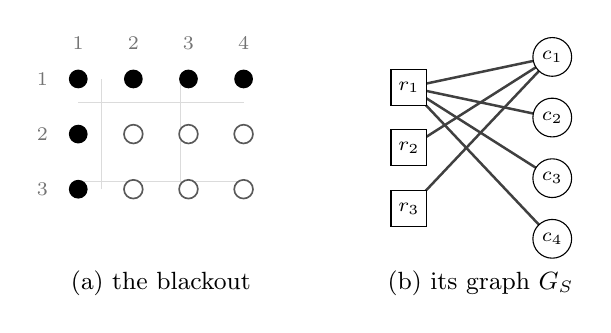
\begin{tikzpicture}[x=0.700cm,y=0.700cm,baseline=(current bounding box.north)]
  \draw[gridcol] (1,-1) grid (4,-3);
  \fill[black] (1,-1) circle (0.17);
  \fill[black] (2,-1) circle (0.17);
  \fill[black] (3,-1) circle (0.17);
  \fill[black] (4,-1) circle (0.17);
  \fill[black] (1,-2) circle (0.17);
  \filldraw[fill=white,draw=keptline,line width=0.6pt] (2,-2) circle (0.17);
  \filldraw[fill=white,draw=keptline,line width=0.6pt] (3,-2) circle (0.17);
  \filldraw[fill=white,draw=keptline,line width=0.6pt] (4,-2) circle (0.17);
  \fill[black] (1,-3) circle (0.17);
  \filldraw[fill=white,draw=keptline,line width=0.6pt] (2,-3) circle (0.17);
  \filldraw[fill=white,draw=keptline,line width=0.6pt] (3,-3) circle (0.17);
  \filldraw[fill=white,draw=keptline,line width=0.6pt] (4,-3) circle (0.17);
  \node[lab] at (1,-0.35) {1};
  \node[lab] at (2,-0.35) {2};
  \node[lab] at (3,-0.35) {3};
  \node[lab] at (4,-0.35) {4};
  \node[lab] at (0.35,-1) {1};
  \node[lab] at (0.35,-2) {2};
  \node[lab] at (0.35,-3) {3};
  \node[capt,anchor=north] at (2.5,-4.3) {(a) the blackout};
  \draw[draw=black!75,line width=0.9pt] (7.0,-1.15) -- (9.6,-0.6);
  \draw[draw=black!75,line width=0.9pt] (7.0,-2.25) -- (9.6,-0.6);
  \draw[draw=black!75,line width=0.9pt] (7.0,-3.3500000000000005) -- (9.6,-0.6);
  \draw[draw=black!75,line width=0.9pt] (7.0,-1.15) -- (9.6,-1.7000000000000002);
  \draw[draw=black!75,line width=0.9pt] (7.0,-1.15) -- (9.6,-2.8000000000000003);
  \draw[draw=black!75,line width=0.9pt] (7.0,-1.15) -- (9.6,-3.9000000000000004);
  \node[rowv] at (7.0,-1.15) {$r_{1}$};
  \node[rowv] at (7.0,-2.25) {$r_{2}$};
  \node[rowv] at (7.0,-3.3500000000000005) {$r_{3}$};
  \node[colv] at (9.6,-0.6) {$c_{1}$};
  \node[colv] at (9.6,-1.7000000000000002) {$c_{2}$};
  \node[colv] at (9.6,-2.8000000000000003) {$c_{3}$};
  \node[colv] at (9.6,-3.9000000000000004) {$c_{4}$};
  \node[capt,anchor=north] at (8.3,-4.3) {(b) its graph $G_S$};
\end{tikzpicture}

\caption{The blackout of Example~\ref{ex:game} and its graph. Row 1 is black in every column,
and column 1 is black in every row.}
\label{fig:incidence}
\end{figure}

An axis-aligned rectangle uses 2 rows $j,j'$ and 2 columns $i,i'$, and its 4 corners are the 4
possible edges between them. If all 4 corners are black, these 4 edges form a cycle
$r_j\,c_i\,r_{j'}\,c_{i'}$ of length 4 in $G_S$. The main lemma of this section says that cycles
of length 4 and 6 are exactly what makes axis-aligned rectangles look alike.

\subsection{Three corners are enough}

\begin{lemma}[three corners suffice]\label{lem:threecorners}
Three corners of a rectangle determine the rectangle. So if 2 rectangles have the same
presentation and it has at least 3 points, the 2 rectangles are equal.
\end{lemma}

\begin{proof}
Let $p,q,r$ be 3 corners of a rectangle. Exactly 1 of them, say $q$, is next to both of the
others, and the angle at $q$ in the triangle $pqr$ is a right angle. A triangle has at most 1
right angle, so the 3 points alone tell us which one is $q$. The fourth corner is then
$p+r-q$. For the second claim, a presentation with at least 3 points contains 3 corners of each
rectangle, the same 3 points, so the 2 rectangles have the same corners.
\end{proof}

\begin{figure}[htbp]
\centering
% generated by make_figures.py; width about 3.6 cm
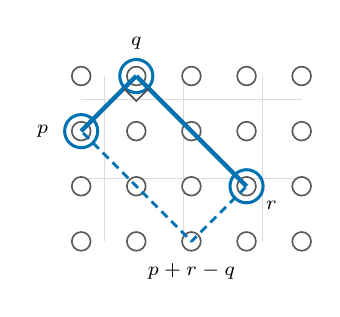
\begin{tikzpicture}[x=0.700cm,y=0.700cm,baseline=(current bounding box.north)]
  \draw[gridcol] (1,-1) grid (5,-4);
  \filldraw[fill=white,draw=keptline,line width=0.6pt] (1,-1) circle (0.17);
  \filldraw[fill=white,draw=keptline,line width=0.6pt] (2,-1) circle (0.17);
  \filldraw[fill=white,draw=keptline,line width=0.6pt] (3,-1) circle (0.17);
  \filldraw[fill=white,draw=keptline,line width=0.6pt] (4,-1) circle (0.17);
  \filldraw[fill=white,draw=keptline,line width=0.6pt] (5,-1) circle (0.17);
  \filldraw[fill=white,draw=keptline,line width=0.6pt] (1,-2) circle (0.17);
  \filldraw[fill=white,draw=keptline,line width=0.6pt] (2,-2) circle (0.17);
  \filldraw[fill=white,draw=keptline,line width=0.6pt] (3,-2) circle (0.17);
  \filldraw[fill=white,draw=keptline,line width=0.6pt] (4,-2) circle (0.17);
  \filldraw[fill=white,draw=keptline,line width=0.6pt] (5,-2) circle (0.17);
  \filldraw[fill=white,draw=keptline,line width=0.6pt] (1,-3) circle (0.17);
  \filldraw[fill=white,draw=keptline,line width=0.6pt] (2,-3) circle (0.17);
  \filldraw[fill=white,draw=keptline,line width=0.6pt] (3,-3) circle (0.17);
  \filldraw[fill=white,draw=keptline,line width=0.6pt] (4,-3) circle (0.17);
  \filldraw[fill=white,draw=keptline,line width=0.6pt] (5,-3) circle (0.17);
  \filldraw[fill=white,draw=keptline,line width=0.6pt] (1,-4) circle (0.17);
  \filldraw[fill=white,draw=keptline,line width=0.6pt] (2,-4) circle (0.17);
  \filldraw[fill=white,draw=keptline,line width=0.6pt] (3,-4) circle (0.17);
  \filldraw[fill=white,draw=keptline,line width=0.6pt] (4,-4) circle (0.17);
  \filldraw[fill=white,draw=keptline,line width=0.6pt] (5,-4) circle (0.17);
  \draw[draw=rectA,line width=1.0pt,line join=round,dash pattern=on 3pt off 2pt] (1,-2) -- (2,-1) -- (4,-3) -- (3,-4) -- cycle;
  \draw[draw=rectA,line width=1.6pt] (2,-1) -- (1,-2);
  \draw[draw=rectA,line width=1.6pt] (2,-1) -- (4,-3);
  \draw[rectA,line width=1.1pt] (1,-2) circle (0.3);
  \draw[rectA,line width=1.1pt] (2,-1) circle (0.3);
  \draw[rectA,line width=1.1pt] (4,-3) circle (0.3);
  \draw[black!70,line width=0.6pt] (1.774,-1.226) -- (2.000,-1.453) -- (2.226,-1.226);
  \node[tiny] at (0.3,-2.0) {$p$};
  \node[tiny] at (2.0,-0.4) {$q$};
  \node[tiny] at (4.45,-3.35) {$r$};
  \node[tiny] at (3.0,-4.55) {$p+r-q$};
\end{tikzpicture}

\caption{The right angle is at $q$, so the missing corner is $p+r-q$.}
\label{fig:threecorners}
\end{figure}

So 2 rectangles can only be confused if both show at most 2 corners. When we check a blackout,
we only need to look at rectangles with at least 2 black corners.

\subsection{Short cycles}

\begin{lemma}[axis-aligned rectangles and short cycles]\label{lem:girth}
Suppose $m\ge3$. No 2 axis-aligned rectangles have the same presentation if and only if $G_S$
has no cycle of length 4 and no cycle of length 6.
\end{lemma}

Before the proof, here are the 2 bad cases.

\begin{figure}[htbp]
\centering
% generated by make_figures.py; width about 6.8 cm
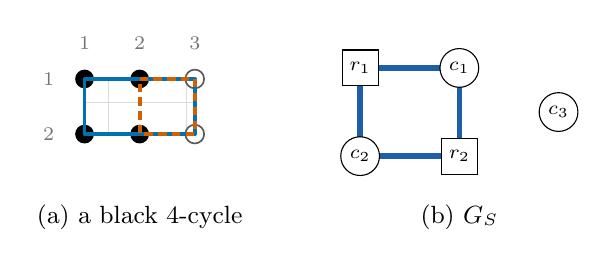
\begin{tikzpicture}[x=0.700cm,y=0.700cm,baseline=(current bounding box.north)]
  \draw[gridcol] (1,-1) grid (3,-2);
  \fill[black] (1,-1) circle (0.17);
  \fill[black] (2,-1) circle (0.17);
  \filldraw[fill=white,draw=keptline,line width=0.6pt] (3,-1) circle (0.17);
  \fill[black] (1,-2) circle (0.17);
  \fill[black] (2,-2) circle (0.17);
  \filldraw[fill=white,draw=keptline,line width=0.6pt] (3,-2) circle (0.17);
  \node[lab] at (1,-0.35) {1};
  \node[lab] at (2,-0.35) {2};
  \node[lab] at (3,-0.35) {3};
  \node[lab] at (0.35,-1) {1};
  \node[lab] at (0.35,-2) {2};
  \draw[draw=rectA,line width=1.4pt,line join=round] (1,-1) -- (3,-1) -- (3,-2) -- (1,-2) -- cycle;
  \draw[draw=rectB,line width=1.4pt,line join=round,dash pattern=on 3pt off 2pt] (2,-1) -- (3,-1) -- (3,-2) -- (2,-2) -- cycle;
  \node[capt,anchor=north] at (2,-3.1) {(a) a black 4-cycle};
  \draw[draw=cyccol,line width=2pt] (6.0,-0.8) -- (7.8,-0.8);
  \draw[draw=cyccol,line width=2pt] (7.8,-2.4) -- (7.8,-0.8);
  \draw[draw=cyccol,line width=2pt] (6.0,-0.8) -- (6.0,-2.4);
  \draw[draw=cyccol,line width=2pt] (7.8,-2.4) -- (6.0,-2.4);
  \node[rowv] at (6.0,-0.8) {$r_{1}$};
  \node[colv] at (7.8,-0.8) {$c_{1}$};
  \node[rowv] at (7.8,-2.4) {$r_{2}$};
  \node[colv] at (6.0,-2.4) {$c_{2}$};
  \node[colv] at (9.6,-1.6) {$c_{3}$};
  \node[capt,anchor=north] at (7.8,-3.1) {(b) $G_S$};
\end{tikzpicture}

\caption{A black 4-cycle: rows 1, 2 and columns 1, 2 are all black. The rectangles $R_{1,3}$ and
$R_{2,3}$ both show the 2 points of column 3.}
\label{fig:c4}
\end{figure}

\begin{example}[4-cycles]
The bad blackout (b) of Example~\ref{ex:2x3} is a black 4-cycle (Figure~\ref{fig:c4}). The
rectangles $R_{1,3}$ and $R_{2,3}$ agree in column 3, and their other columns are fully black,
so they look the same. The same thing happens in any grid with a black 4-cycle on rows $j,j'$
and columns $i,i'$: pick any third column $w$, and the 2 rectangles on rows $j,j'$ with columns
$\{i,w\}$ and $\{i',w\}$ both show only what is white in column $w$. This is where $m\ge3$ is
used.
\end{example}

\begin{figure}[htbp]
\centering
% generated by make_figures.py; width about 6.2 cm
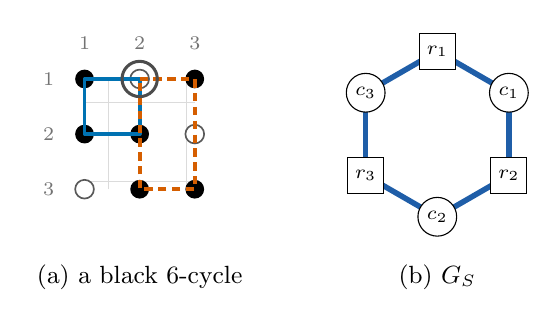
\begin{tikzpicture}[x=0.700cm,y=0.700cm,baseline=(current bounding box.north)]
  \draw[gridcol] (1,-1) grid (3,-3);
  \fill[black] (1,-1) circle (0.17);
  \filldraw[fill=white,draw=keptline,line width=0.6pt] (2,-1) circle (0.17);
  \fill[black] (3,-1) circle (0.17);
  \fill[black] (1,-2) circle (0.17);
  \fill[black] (2,-2) circle (0.17);
  \filldraw[fill=white,draw=keptline,line width=0.6pt] (3,-2) circle (0.17);
  \filldraw[fill=white,draw=keptline,line width=0.6pt] (1,-3) circle (0.17);
  \fill[black] (2,-3) circle (0.17);
  \fill[black] (3,-3) circle (0.17);
  \node[lab] at (1,-0.35) {1};
  \node[lab] at (2,-0.35) {2};
  \node[lab] at (3,-0.35) {3};
  \node[lab] at (0.35,-1) {1};
  \node[lab] at (0.35,-2) {2};
  \node[lab] at (0.35,-3) {3};
  \draw[draw=rectA,line width=1.4pt,line join=round] (1,-1) -- (2,-1) -- (2,-2) -- (1,-2) -- cycle;
  \draw[draw=rectB,line width=1.4pt,line join=round,dash pattern=on 3pt off 2pt] (2,-1) -- (3,-1) -- (3,-3) -- (2,-3) -- cycle;
  \draw[black!70,line width=1.1pt] (2,-1) circle (0.32);
  \node[capt,anchor=north] at (2,-4.2) {(a) a black 6-cycle};
  \draw[draw=cyccol,line width=2pt] (7.4,-0.5) -- (8.699038105676658,-1.25);
  \draw[draw=cyccol,line width=2pt] (8.699038105676658,-2.75) -- (8.699038105676658,-1.25);
  \draw[draw=cyccol,line width=2pt] (8.699038105676658,-2.75) -- (7.4,-3.5);
  \draw[draw=cyccol,line width=2pt] (6.100961894323342,-2.75) -- (7.4,-3.5);
  \draw[draw=cyccol,line width=2pt] (7.4,-0.5) -- (6.100961894323342,-1.2499999999999998);
  \draw[draw=cyccol,line width=2pt] (6.100961894323342,-2.75) -- (6.100961894323342,-1.2499999999999998);
  \node[rowv] at (7.4,-0.5) {$r_{1}$};
  \node[colv] at (8.699038105676658,-1.25) {$c_{1}$};
  \node[rowv] at (8.699038105676658,-2.75) {$r_{2}$};
  \node[colv] at (7.4,-3.5) {$c_{2}$};
  \node[rowv] at (6.100961894323342,-2.75) {$r_{3}$};
  \node[colv] at (6.100961894323342,-1.2499999999999998) {$c_{3}$};
  \node[capt,anchor=north] at (7.4,-4.2) {(b) $G_S$};
\end{tikzpicture}

\caption{A black 6-cycle on the $3\times3$ grid. The solid and the dashed rectangle both show
only the ringed point $(2,1)$.}
\label{fig:c6}
\end{figure}

\begin{example}[6-cycles]
In Figure~\ref{fig:c6} the black points $(1,1),(1,2),(2,2),(2,3),(3,3),(3,1)$ form the cycle
$r_1c_1r_2c_2r_3c_3$ in $G_S$. The rectangle on rows $\{1,2\}$ and columns $\{1,2\}$ has corners
$(1,1),(2,1),(1,2),(2,2)$, and only $(2,1)$ is white. The rectangle on rows $\{1,3\}$ and columns
$\{2,3\}$ has corners $(2,1),(3,1),(2,3),(3,3)$, and again only $(2,1)$ is white. So both show
just $(2,1)$.
\end{example}

\begin{proof}[Proof of Lemma~\ref{lem:girth}]
The 2 examples show the ``only if'' direction in general. For a 4-cycle, see the example above.
For a 6-cycle $r_a\,c_x\,r_b\,c_y\,r_c\,c_z$, the black points are $(x,a),(x,b),(y,b),(y,c),
(z,c),(z,a)$. The rectangle on rows $\{a,b\}$ and columns $\{x,y\}$ and the rectangle on rows
$\{a,c\}$ and columns $\{y,z\}$ are different, and every corner of each is black except
possibly the shared corner $(y,a)$. So they have the same presentation.

For the ``if'' direction, assume $G_S$ has no 4-cycle and no 6-cycle. Let $R_1\ne R_2$ be
axis-aligned rectangles with the same presentation $P$. We get a contradiction in each case.
\begin{itemize}[leftmargin=*,itemsep=1pt]
\item $|P|\ge3$: Lemma~\ref{lem:threecorners} gives $R_1=R_2$.
\item $|P|=0$: all 4 corners of $R_1$ are black, and they form a 4-cycle.
\item $|P|=2$, the 2 points in different rows and different columns: then they are opposite
corners of both rectangles, and 2 opposite corners determine an axis-aligned rectangle, so
$R_1=R_2$.
\item $|P|=2$, the 2 points in 1 row $a$, at columns $x$ and $y$: then $R_1$ uses rows
$\{a,b\}$ and $R_2$ uses rows $\{a,c\}$ with $b\ne c$, and the points
$(x,b),(y,b),(x,c),(y,c)$ are all black. That is the 4-cycle $r_b\,c_x\,r_c\,c_y$. The case of
1 column is the same with rows and columns swapped.
\item $|P|=1$, say $P=\{(x,a)\}$: write $R_1$ as rows $\{a,b\}$, columns $\{x,y\}$ and $R_2$ as
rows $\{a,c\}$, columns $\{x,z\}$. The black points are $(y,a),(x,b),(y,b)$ and
$(z,a),(x,c),(z,c)$. If $b=c$ then $y\ne z$, and rows $a,b$ with columns $y,z$ are all black, a
4-cycle. If $y=z$, then in the same way rows $b,c$ with columns $x,y$ give a 4-cycle. Otherwise
the 6 black points form the 6-cycle $r_a\,c_y\,r_b\,c_x\,r_c\,c_z$.
\end{itemize}
Every case is impossible, so $R_1$ and $R_2$ can't have the same presentation.
\end{proof}

Note that the lemma is only about axis-aligned rectangles against each other. A tilted rectangle
could still be confused with something, and we deal with that separately for each grid.

%======================================================================
\section{An upper bound for every grid}\label{sec:rowbound}

\begin{theorem}[row bound]\label{thm:rowbound}
Let $m\ge3$. Every valid blackout of an $n\times m$ grid has at most $m+\lfloor n^2/4\rfloor$
points. If also $n\ge3$, then by swapping rows and columns it has at most
$n+\lfloor m^2/4\rfloor$ points.
\end{theorem}

The plan is to turn $G_S$ into a graph $H$ on the rows alone, with no triangles, and then use
Mantel's theorem, which says a triangle-free graph on $n$ vertices has at most $n^2/4$ edges.

\subsection{Building the graph $H$}

For each column $i$ let $B_i$ be the set of rows where column $i$ is black. If $B_i$ is not
empty, join the rows in $B_i$ by any tree (for example a path from top to bottom). A tree on
$|B_i|$ vertices has $|B_i|-1$ edges, so a column with 1 black point adds no edges. Put the
trees of all the columns together on the same $n$ row vertices, and call the result $H$.

\begin{figure}[htbp]
\centering
% generated by make_figures.py; width about 10.8 cm
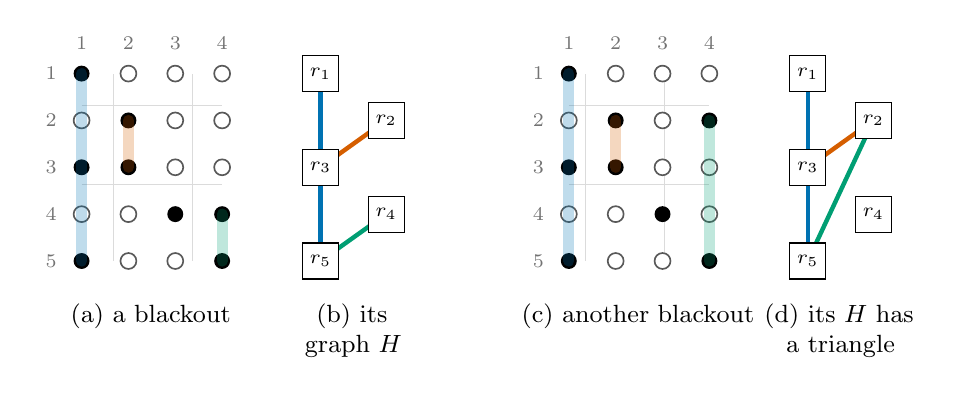
\begin{tikzpicture}[x=0.595cm,y=0.595cm,baseline=(current bounding box.north)]
  \draw[gridcol] (1,-1) grid (4,-5);
  \fill[black] (1,-1) circle (0.17);
  \filldraw[fill=white,draw=keptline,line width=0.6pt] (2,-1) circle (0.17);
  \filldraw[fill=white,draw=keptline,line width=0.6pt] (3,-1) circle (0.17);
  \filldraw[fill=white,draw=keptline,line width=0.6pt] (4,-1) circle (0.17);
  \filldraw[fill=white,draw=keptline,line width=0.6pt] (1,-2) circle (0.17);
  \fill[black] (2,-2) circle (0.17);
  \filldraw[fill=white,draw=keptline,line width=0.6pt] (3,-2) circle (0.17);
  \filldraw[fill=white,draw=keptline,line width=0.6pt] (4,-2) circle (0.17);
  \fill[black] (1,-3) circle (0.17);
  \fill[black] (2,-3) circle (0.17);
  \filldraw[fill=white,draw=keptline,line width=0.6pt] (3,-3) circle (0.17);
  \filldraw[fill=white,draw=keptline,line width=0.6pt] (4,-3) circle (0.17);
  \filldraw[fill=white,draw=keptline,line width=0.6pt] (1,-4) circle (0.17);
  \filldraw[fill=white,draw=keptline,line width=0.6pt] (2,-4) circle (0.17);
  \fill[black] (3,-4) circle (0.17);
  \fill[black] (4,-4) circle (0.17);
  \fill[black] (1,-5) circle (0.17);
  \filldraw[fill=white,draw=keptline,line width=0.6pt] (2,-5) circle (0.17);
  \filldraw[fill=white,draw=keptline,line width=0.6pt] (3,-5) circle (0.17);
  \fill[black] (4,-5) circle (0.17);
  \node[lab] at (1,-0.35) {1};
  \node[lab] at (2,-0.35) {2};
  \node[lab] at (3,-0.35) {3};
  \node[lab] at (4,-0.35) {4};
  \node[lab] at (0.35,-1) {1};
  \node[lab] at (0.35,-2) {2};
  \node[lab] at (0.35,-3) {3};
  \node[lab] at (0.35,-4) {4};
  \node[lab] at (0.35,-5) {5};
  \draw[rectA,line width=4pt,opacity=0.25,line cap=round] (1,-1) -- (1,-5);
  \draw[rectB,line width=4pt,opacity=0.25,line cap=round] (2,-2) -- (2,-3);
  \draw[rectC,line width=4pt,opacity=0.25,line cap=round] (4,-4) -- (4,-5);
  \draw[gridcol] (11.4,-1) grid (14.4,-5);
  \fill[black] (11.4,-1) circle (0.17);
  \filldraw[fill=white,draw=keptline,line width=0.6pt] (12.4,-1) circle (0.17);
  \filldraw[fill=white,draw=keptline,line width=0.6pt] (13.4,-1) circle (0.17);
  \filldraw[fill=white,draw=keptline,line width=0.6pt] (14.4,-1) circle (0.17);
  \filldraw[fill=white,draw=keptline,line width=0.6pt] (11.4,-2) circle (0.17);
  \fill[black] (12.4,-2) circle (0.17);
  \filldraw[fill=white,draw=keptline,line width=0.6pt] (13.4,-2) circle (0.17);
  \fill[black] (14.4,-2) circle (0.17);
  \fill[black] (11.4,-3) circle (0.17);
  \fill[black] (12.4,-3) circle (0.17);
  \filldraw[fill=white,draw=keptline,line width=0.6pt] (13.4,-3) circle (0.17);
  \filldraw[fill=white,draw=keptline,line width=0.6pt] (14.4,-3) circle (0.17);
  \filldraw[fill=white,draw=keptline,line width=0.6pt] (11.4,-4) circle (0.17);
  \filldraw[fill=white,draw=keptline,line width=0.6pt] (12.4,-4) circle (0.17);
  \fill[black] (13.4,-4) circle (0.17);
  \filldraw[fill=white,draw=keptline,line width=0.6pt] (14.4,-4) circle (0.17);
  \fill[black] (11.4,-5) circle (0.17);
  \filldraw[fill=white,draw=keptline,line width=0.6pt] (12.4,-5) circle (0.17);
  \filldraw[fill=white,draw=keptline,line width=0.6pt] (13.4,-5) circle (0.17);
  \fill[black] (14.4,-5) circle (0.17);
  \node[lab] at (11.4,-0.35) {1};
  \node[lab] at (12.4,-0.35) {2};
  \node[lab] at (13.4,-0.35) {3};
  \node[lab] at (14.4,-0.35) {4};
  \node[lab] at (10.75,-1) {1};
  \node[lab] at (10.75,-2) {2};
  \node[lab] at (10.75,-3) {3};
  \node[lab] at (10.75,-4) {4};
  \node[lab] at (10.75,-5) {5};
  \draw[rectA,line width=4pt,opacity=0.25,line cap=round] (11.4,-1) -- (11.4,-5);
  \draw[rectB,line width=4pt,opacity=0.25,line cap=round] (12.4,-2) -- (12.4,-3);
  \draw[rectC,line width=4pt,opacity=0.25,line cap=round] (14.4,-2) -- (14.4,-5);
  \draw[rectA,line width=1.6pt] (6.1000000000000005,-1) -- (6.1000000000000005,-3);
  \draw[rectA,line width=1.6pt] (6.1000000000000005,-3) -- (6.1000000000000005,-5);
  \draw[rectB,line width=1.6pt] (7.5,-2) -- (6.1000000000000005,-3);
  \draw[rectC,line width=1.6pt] (7.5,-4) -- (6.1000000000000005,-5);
  \node[rowv] at (6.1000000000000005,-1) {$r_{1}$};
  \node[rowv] at (7.5,-2) {$r_{2}$};
  \node[rowv] at (6.1000000000000005,-3) {$r_{3}$};
  \node[rowv] at (7.5,-4) {$r_{4}$};
  \node[rowv] at (6.1000000000000005,-5) {$r_{5}$};
  \draw[rectA,line width=1.6pt] (16.5,-1) -- (16.5,-3);
  \draw[rectA,line width=1.6pt] (16.5,-3) -- (16.5,-5);
  \draw[rectB,line width=1.6pt] (17.9,-2) -- (16.5,-3);
  \draw[rectC,line width=1.6pt] (17.9,-2) -- (16.5,-5);
  \node[rowv] at (16.5,-1) {$r_{1}$};
  \node[rowv] at (17.9,-2) {$r_{2}$};
  \node[rowv] at (16.5,-3) {$r_{3}$};
  \node[rowv] at (17.9,-4) {$r_{4}$};
  \node[rowv] at (16.5,-5) {$r_{5}$};
  \node[capt,anchor=north,text width=2.92cm,align=center] at (2.5,-5.7) {(a) a blackout};
  \node[capt,anchor=north,text width=1.96cm,align=center] at (6.800000000000001,-5.7) {(b) its graph $H$};
  \node[capt,anchor=north,text width=2.92cm,align=center] at (12.9,-5.7) {(c) another blackout};
  \node[capt,anchor=north,text width=1.96cm,align=center] at (17.2,-5.7) {(d) its $H$ has a triangle};
\end{tikzpicture}

\caption{(a) A blackout of the $5\times4$ grid, with the black points of each column joined.
(b) The graph $H$: each column with 2 or more black points contributes a path on its black rows,
in the same colour. (c), (d) The same with column 4 moved to rows 2 and 5, which creates a
triangle in $H$.}
\label{fig:rowbound}
\end{figure}

\begin{example}
In Figure~\ref{fig:rowbound}(a), column 1 is black in rows $1,3,5$, column 2 in rows $2,3$,
column 3 in row $4$ and column 4 in rows $4,5$. In (b), column 1 gives the path $r_1r_3r_5$,
column 2 gives the edge $r_2r_3$, column 3 gives nothing and column 4 gives $r_4r_5$. The result
is a tree with 4 edges. Count the black points column by column: each non-empty column has 1
point for its first row and 1 more for each edge of its tree, so
$|S|=4+4=8$ (4 non-empty columns, 4 edges of $H$).

In (c), column 4 is black in rows $2$ and $5$ instead, and $H$ gets the edge $r_2r_5$. Now $H$
has the triangle $r_2r_3r_5$, with its 3 edges coming from 3 different columns. Go back to the
grid and this triangle is the black 6-cycle $r_3\,c_1\,r_5\,c_4\,r_2\,c_2$, through the points
$(1,3),(1,5),(4,5),(4,2),(2,2),(2,3)$. By Lemma~\ref{lem:girth} that blackout is not valid.
\end{example}

The example shows the general facts we need.

\begin{lemma}\label{lem:H}
If $S$ is valid and $m\ge3$, then $H$ has no repeated edges and no triangles, and
$|S|=t+e(H)$, where $t$ is the number of non-empty columns and $e(H)$ the number of edges of $H$.
\end{lemma}

\begin{proof}
By Lemma~\ref{lem:girth}, $G_S$ has no 4-cycle and no 6-cycle.

\emph{No repeated edges.} One tree never uses the same edge twice. If 2 different columns $i,i'$
both gave the edge $r_jr_{j'}$, both columns would be black in rows $j$ and $j'$, which is the
4-cycle $r_j\,c_i\,r_{j'}\,c_{i'}$.

\emph{No triangles.} Suppose $r_ar_br_c$ is a triangle in $H$. The 3 edges can't all come from 1
column, because a tree has no cycles. If 2 come from column $i$ and the third from column
$i'\ne i$, then all of $a,b,c$ are in $B_i$, and the third edge puts 2 of them in $B_{i'}$; so
columns $i,i'$ share 2 black rows, a 4-cycle. If the 3 edges come from 3 different columns
$i$ ($r_ar_b$), $i'$ ($r_br_c$) and $i''$ ($r_ar_c$), then $r_a\,c_i\,r_b\,c_{i'}\,r_c\,c_{i''}$
is a 6-cycle in $G_S$.

\emph{The count.} $e(H)=\sum_{B_i\ne\emptyset}(|B_i|-1)=|S|-t$.
\end{proof}

\subsection{Mantel's theorem}

\begin{lemma}[Mantel]\label{lem:mantel}
A graph on $n$ vertices with no triangle and no repeated edges has at most $\lfloor n^2/4\rfloor$
edges.
\end{lemma}

\begin{figure}[htbp]
\centering
% generated by make_figures.py; width about 8.6 cm
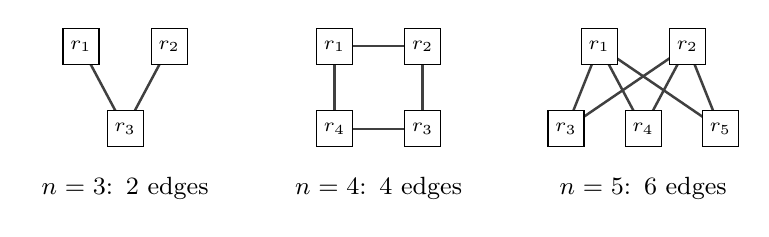
\begin{tikzpicture}[x=0.700cm,y=0.700cm,baseline=(current bounding box.north)]
  \draw[draw=black!75,line width=0.9pt] (0,-1) -- (0.8,-2.5);
  \draw[draw=black!75,line width=0.9pt] (1.6,-1) -- (0.8,-2.5);
  \node[rowv] at (0,-1) {$r_{1}$};
  \node[rowv] at (1.6,-1) {$r_{2}$};
  \node[rowv] at (0.8,-2.5) {$r_{3}$};
  \node[capt,anchor=north,text width=2.24cm,align=center] at (0.8,-3.2) {$n=3$: 2 edges};
  \draw[draw=black!75,line width=0.9pt] (4.6,-1) -- (6.2,-1);
  \draw[draw=black!75,line width=0.9pt] (6.2,-1) -- (6.2,-2.5);
  \draw[draw=black!75,line width=0.9pt] (6.2,-2.5) -- (4.6,-2.5);
  \draw[draw=black!75,line width=0.9pt] (4.6,-2.5) -- (4.6,-1);
  \node[rowv] at (4.6,-1) {$r_{1}$};
  \node[rowv] at (6.2,-1) {$r_{2}$};
  \node[rowv] at (6.2,-2.5) {$r_{3}$};
  \node[rowv] at (4.6,-2.5) {$r_{4}$};
  \node[capt,anchor=north,text width=2.24cm,align=center] at (5.4,-3.2) {$n=4$: 4 edges};
  \draw[draw=black!75,line width=0.9pt] (9.4,-1) -- (8.8,-2.5);
  \draw[draw=black!75,line width=0.9pt] (9.4,-1) -- (10.2,-2.5);
  \draw[draw=black!75,line width=0.9pt] (9.4,-1) -- (11.6,-2.5);
  \draw[draw=black!75,line width=0.9pt] (11.0,-1) -- (8.8,-2.5);
  \draw[draw=black!75,line width=0.9pt] (11.0,-1) -- (10.2,-2.5);
  \draw[draw=black!75,line width=0.9pt] (11.0,-1) -- (11.6,-2.5);
  \node[rowv] at (9.4,-1) {$r_{1}$};
  \node[rowv] at (11.0,-1) {$r_{2}$};
  \node[rowv] at (8.8,-2.5) {$r_{3}$};
  \node[rowv] at (10.2,-2.5) {$r_{4}$};
  \node[rowv] at (11.6,-2.5) {$r_{5}$};
  \node[capt,anchor=north,text width=2.24cm,align=center] at (10.2,-3.2) {$n=5$: 6 edges};
\end{tikzpicture}

\caption{Triangle-free graphs with the most edges for $n=3,4,5$: split the vertices into 2
nearly equal groups and join every pair across.}
\label{fig:mantel}
\end{figure}

\begin{proof}
Let the graph have $e$ edges, and write $d(v)$ for the degree of $v$. If $e=0$ there is nothing
to prove. For an edge $uv$, the neighbours of $u$ and the neighbours of $v$ don't overlap (a
common neighbour would make a triangle), so $d(u)+d(v)\le n$. Add this up over all $e$ edges.
Each vertex $v$ appears once for each of its $d(v)$ edges, so the left side adds up to
$\sum_vd(v)^2$, and
\[
\sum_v d(v)^2\le ne.
\]
On the other hand $\sum_vd(v)=2e$, so by the Cauchy--Schwarz inequality
$\sum_vd(v)^2\ge(2e)^2/n$. Together, $4e^2/n\le ne$, so $e\le n^2/4$, and since $e$ is a whole
number, $e\le\lfloor n^2/4\rfloor$.
\end{proof}

\begin{proof}[Proof of Theorem~\ref{thm:rowbound}]
By Lemma~\ref{lem:H}, $|S|=t+e(H)$ with $t\le m$, and $H$ is triangle-free on $n$ vertices, so
$e(H)\le\lfloor n^2/4\rfloor$ by Mantel. Hence $|S|\le m+\lfloor n^2/4\rfloor$. Everything so far
is symmetric in rows and columns except where Lemma~\ref{lem:girth} needed a third column, so if
$n\ge3$ the same argument with rows and columns swapped gives $|S|\le n+\lfloor m^2/4\rfloor$.
\end{proof}

For 2, 3 and 4 rows this gives $m+1$, $m+2$ and $m+4$. On 2 rows that is the Strip Theorem's
value. On 3 rows and on 4 rows with $m\ge6$ it is also exact, and the next sections show it.

%======================================================================
\section{Tilted rectangles on 3 and 4 rows}\label{sec:tilted}

To use the row bound on narrow grids we still need to handle tilted rectangles. On 3 or 4 rows
there are only a few kinds.

For $1\le i\le m-2$ and $1\le j\le n-2$, the \emph{diamond} is the tilted square
\[
D(i,j)=\{(i,j+1),\,(i+1,j),\,(i+2,j+1),\,(i+1,j+2)\}.
\]
For $1\le i\le m-3$, define 4 more kinds on 4 rows:
\begin{align*}
A_i&=\{(i,3),(i+1,4),(i+2,1),(i+3,2)\}, & B_i&=\{(i,3),(i+2,4),(i+1,1),(i+3,2)\},\\
C_i&=\{(i,2),(i+1,4),(i+2,1),(i+3,3)\}, & E_i&=\{(i,2),(i+2,4),(i+1,1),(i+3,3)\}.
\end{align*}

\begin{figure}[htbp]
\centering
% generated by make_figures.py; width about 15.1 cm
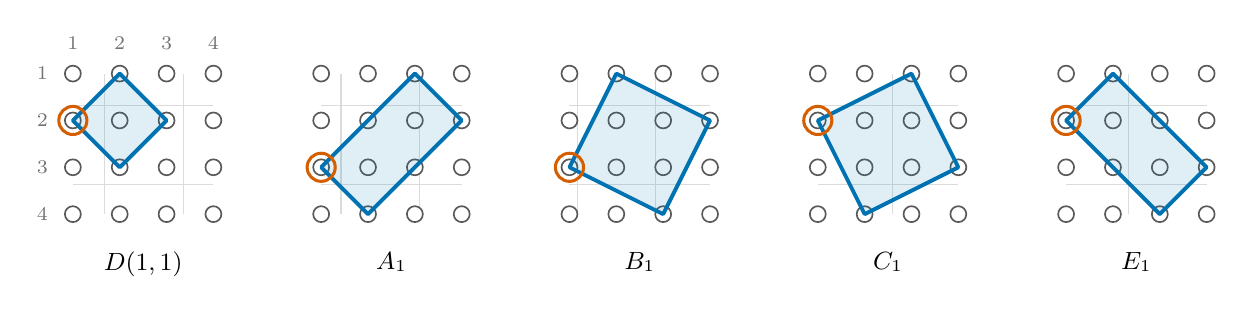
\begin{tikzpicture}[x=0.595cm,y=0.595cm,baseline=(current bounding box.north)]
  \draw[gridcol] (1.0,-1) grid (4.0,-4);
  \filldraw[fill=white,draw=keptline,line width=0.6pt] (1.0,-1) circle (0.17);
  \filldraw[fill=white,draw=keptline,line width=0.6pt] (2.0,-1) circle (0.17);
  \filldraw[fill=white,draw=keptline,line width=0.6pt] (3.0,-1) circle (0.17);
  \filldraw[fill=white,draw=keptline,line width=0.6pt] (4.0,-1) circle (0.17);
  \filldraw[fill=white,draw=keptline,line width=0.6pt] (1.0,-2) circle (0.17);
  \filldraw[fill=white,draw=keptline,line width=0.6pt] (2.0,-2) circle (0.17);
  \filldraw[fill=white,draw=keptline,line width=0.6pt] (3.0,-2) circle (0.17);
  \filldraw[fill=white,draw=keptline,line width=0.6pt] (4.0,-2) circle (0.17);
  \filldraw[fill=white,draw=keptline,line width=0.6pt] (1.0,-3) circle (0.17);
  \filldraw[fill=white,draw=keptline,line width=0.6pt] (2.0,-3) circle (0.17);
  \filldraw[fill=white,draw=keptline,line width=0.6pt] (3.0,-3) circle (0.17);
  \filldraw[fill=white,draw=keptline,line width=0.6pt] (4.0,-3) circle (0.17);
  \filldraw[fill=white,draw=keptline,line width=0.6pt] (1.0,-4) circle (0.17);
  \filldraw[fill=white,draw=keptline,line width=0.6pt] (2.0,-4) circle (0.17);
  \filldraw[fill=white,draw=keptline,line width=0.6pt] (3.0,-4) circle (0.17);
  \filldraw[fill=white,draw=keptline,line width=0.6pt] (4.0,-4) circle (0.17);
  \node[lab] at (1.0,-0.35) {1};
  \node[lab] at (2.0,-0.35) {2};
  \node[lab] at (3.0,-0.35) {3};
  \node[lab] at (4.0,-0.35) {4};
  \node[lab] at (0.35,-1) {1};
  \node[lab] at (0.35,-2) {2};
  \node[lab] at (0.35,-3) {3};
  \node[lab] at (0.35,-4) {4};
  \fill[rectA,opacity=0.12] (2.0,-1) -- (3.0,-2) -- (2.0,-3) -- (1.0,-2) -- cycle;
  \draw[draw=rectA,line width=1.4pt,line join=round] (2.0,-1) -- (3.0,-2) -- (2.0,-3) -- (1.0,-2) -- cycle;
  \draw[rectB,line width=1.1pt] (1.0,-2) circle (0.3);
  \node[capt,anchor=north] at (2.5,-4.6) {$D(1,1)$};
  \draw[gridcol] (6.3,-1) grid (9.3,-4);
  \filldraw[fill=white,draw=keptline,line width=0.6pt] (6.3,-1) circle (0.17);
  \filldraw[fill=white,draw=keptline,line width=0.6pt] (7.3,-1) circle (0.17);
  \filldraw[fill=white,draw=keptline,line width=0.6pt] (8.3,-1) circle (0.17);
  \filldraw[fill=white,draw=keptline,line width=0.6pt] (9.3,-1) circle (0.17);
  \filldraw[fill=white,draw=keptline,line width=0.6pt] (6.3,-2) circle (0.17);
  \filldraw[fill=white,draw=keptline,line width=0.6pt] (7.3,-2) circle (0.17);
  \filldraw[fill=white,draw=keptline,line width=0.6pt] (8.3,-2) circle (0.17);
  \filldraw[fill=white,draw=keptline,line width=0.6pt] (9.3,-2) circle (0.17);
  \filldraw[fill=white,draw=keptline,line width=0.6pt] (6.3,-3) circle (0.17);
  \filldraw[fill=white,draw=keptline,line width=0.6pt] (7.3,-3) circle (0.17);
  \filldraw[fill=white,draw=keptline,line width=0.6pt] (8.3,-3) circle (0.17);
  \filldraw[fill=white,draw=keptline,line width=0.6pt] (9.3,-3) circle (0.17);
  \filldraw[fill=white,draw=keptline,line width=0.6pt] (6.3,-4) circle (0.17);
  \filldraw[fill=white,draw=keptline,line width=0.6pt] (7.3,-4) circle (0.17);
  \filldraw[fill=white,draw=keptline,line width=0.6pt] (8.3,-4) circle (0.17);
  \filldraw[fill=white,draw=keptline,line width=0.6pt] (9.3,-4) circle (0.17);
  \fill[rectA,opacity=0.12] (8.3,-1) -- (9.3,-2) -- (7.3,-4) -- (6.3,-3) -- cycle;
  \draw[draw=rectA,line width=1.4pt,line join=round] (8.3,-1) -- (9.3,-2) -- (7.3,-4) -- (6.3,-3) -- cycle;
  \draw[rectB,line width=1.1pt] (6.3,-3) circle (0.3);
  \node[capt,anchor=north] at (7.8,-4.6) {$A_1$};
  \draw[gridcol] (11.6,-1) grid (14.6,-4);
  \filldraw[fill=white,draw=keptline,line width=0.6pt] (11.6,-1) circle (0.17);
  \filldraw[fill=white,draw=keptline,line width=0.6pt] (12.6,-1) circle (0.17);
  \filldraw[fill=white,draw=keptline,line width=0.6pt] (13.6,-1) circle (0.17);
  \filldraw[fill=white,draw=keptline,line width=0.6pt] (14.6,-1) circle (0.17);
  \filldraw[fill=white,draw=keptline,line width=0.6pt] (11.6,-2) circle (0.17);
  \filldraw[fill=white,draw=keptline,line width=0.6pt] (12.6,-2) circle (0.17);
  \filldraw[fill=white,draw=keptline,line width=0.6pt] (13.6,-2) circle (0.17);
  \filldraw[fill=white,draw=keptline,line width=0.6pt] (14.6,-2) circle (0.17);
  \filldraw[fill=white,draw=keptline,line width=0.6pt] (11.6,-3) circle (0.17);
  \filldraw[fill=white,draw=keptline,line width=0.6pt] (12.6,-3) circle (0.17);
  \filldraw[fill=white,draw=keptline,line width=0.6pt] (13.6,-3) circle (0.17);
  \filldraw[fill=white,draw=keptline,line width=0.6pt] (14.6,-3) circle (0.17);
  \filldraw[fill=white,draw=keptline,line width=0.6pt] (11.6,-4) circle (0.17);
  \filldraw[fill=white,draw=keptline,line width=0.6pt] (12.6,-4) circle (0.17);
  \filldraw[fill=white,draw=keptline,line width=0.6pt] (13.6,-4) circle (0.17);
  \filldraw[fill=white,draw=keptline,line width=0.6pt] (14.6,-4) circle (0.17);
  \fill[rectA,opacity=0.12] (12.6,-1) -- (14.6,-2) -- (13.6,-4) -- (11.6,-3) -- cycle;
  \draw[draw=rectA,line width=1.4pt,line join=round] (12.6,-1) -- (14.6,-2) -- (13.6,-4) -- (11.6,-3) -- cycle;
  \draw[rectB,line width=1.1pt] (11.6,-3) circle (0.3);
  \node[capt,anchor=north] at (13.1,-4.6) {$B_1$};
  \draw[gridcol] (16.9,-1) grid (19.9,-4);
  \filldraw[fill=white,draw=keptline,line width=0.6pt] (16.9,-1) circle (0.17);
  \filldraw[fill=white,draw=keptline,line width=0.6pt] (17.9,-1) circle (0.17);
  \filldraw[fill=white,draw=keptline,line width=0.6pt] (18.9,-1) circle (0.17);
  \filldraw[fill=white,draw=keptline,line width=0.6pt] (19.9,-1) circle (0.17);
  \filldraw[fill=white,draw=keptline,line width=0.6pt] (16.9,-2) circle (0.17);
  \filldraw[fill=white,draw=keptline,line width=0.6pt] (17.9,-2) circle (0.17);
  \filldraw[fill=white,draw=keptline,line width=0.6pt] (18.9,-2) circle (0.17);
  \filldraw[fill=white,draw=keptline,line width=0.6pt] (19.9,-2) circle (0.17);
  \filldraw[fill=white,draw=keptline,line width=0.6pt] (16.9,-3) circle (0.17);
  \filldraw[fill=white,draw=keptline,line width=0.6pt] (17.9,-3) circle (0.17);
  \filldraw[fill=white,draw=keptline,line width=0.6pt] (18.9,-3) circle (0.17);
  \filldraw[fill=white,draw=keptline,line width=0.6pt] (19.9,-3) circle (0.17);
  \filldraw[fill=white,draw=keptline,line width=0.6pt] (16.9,-4) circle (0.17);
  \filldraw[fill=white,draw=keptline,line width=0.6pt] (17.9,-4) circle (0.17);
  \filldraw[fill=white,draw=keptline,line width=0.6pt] (18.9,-4) circle (0.17);
  \filldraw[fill=white,draw=keptline,line width=0.6pt] (19.9,-4) circle (0.17);
  \fill[rectA,opacity=0.12] (16.9,-2) -- (18.9,-1) -- (19.9,-3) -- (17.9,-4) -- cycle;
  \draw[draw=rectA,line width=1.4pt,line join=round] (16.9,-2) -- (18.9,-1) -- (19.9,-3) -- (17.9,-4) -- cycle;
  \draw[rectB,line width=1.1pt] (16.9,-2) circle (0.3);
  \node[capt,anchor=north] at (18.4,-4.6) {$C_1$};
  \draw[gridcol] (22.2,-1) grid (25.2,-4);
  \filldraw[fill=white,draw=keptline,line width=0.6pt] (22.2,-1) circle (0.17);
  \filldraw[fill=white,draw=keptline,line width=0.6pt] (23.2,-1) circle (0.17);
  \filldraw[fill=white,draw=keptline,line width=0.6pt] (24.2,-1) circle (0.17);
  \filldraw[fill=white,draw=keptline,line width=0.6pt] (25.2,-1) circle (0.17);
  \filldraw[fill=white,draw=keptline,line width=0.6pt] (22.2,-2) circle (0.17);
  \filldraw[fill=white,draw=keptline,line width=0.6pt] (23.2,-2) circle (0.17);
  \filldraw[fill=white,draw=keptline,line width=0.6pt] (24.2,-2) circle (0.17);
  \filldraw[fill=white,draw=keptline,line width=0.6pt] (25.2,-2) circle (0.17);
  \filldraw[fill=white,draw=keptline,line width=0.6pt] (22.2,-3) circle (0.17);
  \filldraw[fill=white,draw=keptline,line width=0.6pt] (23.2,-3) circle (0.17);
  \filldraw[fill=white,draw=keptline,line width=0.6pt] (24.2,-3) circle (0.17);
  \filldraw[fill=white,draw=keptline,line width=0.6pt] (25.2,-3) circle (0.17);
  \filldraw[fill=white,draw=keptline,line width=0.6pt] (22.2,-4) circle (0.17);
  \filldraw[fill=white,draw=keptline,line width=0.6pt] (23.2,-4) circle (0.17);
  \filldraw[fill=white,draw=keptline,line width=0.6pt] (24.2,-4) circle (0.17);
  \filldraw[fill=white,draw=keptline,line width=0.6pt] (25.2,-4) circle (0.17);
  \fill[rectA,opacity=0.12] (22.2,-2) -- (23.2,-1) -- (25.2,-3) -- (24.2,-4) -- cycle;
  \draw[draw=rectA,line width=1.4pt,line join=round] (22.2,-2) -- (23.2,-1) -- (25.2,-3) -- (24.2,-4) -- cycle;
  \draw[rectB,line width=1.1pt] (22.2,-2) circle (0.3);
  \node[capt,anchor=north] at (23.7,-4.6) {$E_1$};
\end{tikzpicture}

\caption{The diamond $D=D(1,1)$ and the 4 other kinds $A_1,B_1,C_1,E_1$, in a $4\times4$
window. The ringed corner is the leftmost one.}
\label{fig:tilted}
\end{figure}

\begin{lemma}[tilted rectangles on narrow grids]\label{lem:tilted}
On 3 rows, the tilted rectangles are exactly the diamonds $D(i,1)$. On 4 rows, they are exactly
the diamonds $D(i,1)$ and $D(i,2)$ and the rectangles $A_i,B_i,C_i,E_i$.
\end{lemma}

\begin{proof}
First, a tilted rectangle has exactly 1 leftmost corner. Suppose 2 corners both have the
smallest column number $x_0$. They aren't next to each other, since no side of a tilted
rectangle is vertical, so they are opposite corners and the centre of the rectangle is in
column $x_0$. The other 2 corners have the same centre, so their column numbers add up to
$2x_0$. Both are at least $x_0$, so both equal $x_0$, and then all 4 corners are on 1 vertical
line, which is impossible.

From the leftmost corner both sides go to the right. They are at right angles, so one goes up
and the other goes down. Write them as $(a,-b)$ (up and right) and $(c,d)$ (down and right),
where $a,b,c,d$ are positive integers. Being at right angles means $ac-bd=0$, so $ac=bd$. The
corners use the rows from (leftmost row $-\,b$) to (leftmost row $+\,d$), so the rectangle
covers $b+d+1$ rows.

On 3 rows, $b+d+1\le3$, so $b=d=1$, then $ac=1$ gives $a=c=1$, and the rectangle is a diamond.
On 4 rows, either $b=d=1$ again (a diamond), or $b+d=3$, so $\{b,d\}=\{1,2\}$, $ac=bd=2$ and
$\{a,c\}=\{1,2\}$. These are 4 choices, and they are the 4 kinds:
\begin{center}
\begin{tabular}{ccccc}
\toprule
 & $A$ & $B$ & $C$ & $E$\\
\midrule
side going up, $(a,-b)$ & $(2,-2)$ & $(1,-2)$ & $(2,-1)$ & $(1,-1)$ \\
side going down, $(c,d)$ & $(1,1)$ & $(2,1)$ & $(1,2)$ & $(2,2)$ \\
\bottomrule
\end{tabular}
\end{center}
The leftmost corner is then forced into row 3 for $A,B$ (it needs 2 rows above and 1 below) and
row 2 for $C,E$, which gives the formulas above.
\end{proof}

So the $4\times4$ grid has 8 tilted rectangles: $D(1,1),D(2,1),D(1,2),D(2,2),A_1,B_1,C_1,E_1$.
Note that $B$ and $C$ are tilted squares with side $\sqrt5$, while $A$ and $E$ have sides
$\sqrt2$ and $2\sqrt2$.

%======================================================================
\section{Three rows}\label{sec:three}

\begin{theorem}[Three-Row Theorem]\label{thm:threerow}
For every $m\ge3$, the maximum blackout of the $3\times m$ grid is $m+2$.
\end{theorem}

The upper bound is the row bound, $m+\lfloor9/4\rfloor=m+2$. For the lower bound we black out
all of row 1 and all of column 1:
\[
S=\{(i,1):1\le i\le m\}\cup\{(1,2),(1,3)\}.
\]
This has $m+2$ points. It is the blackout of Example~\ref{ex:game}, now on a longer grid.

\begin{figure}[htbp]
\centering
% generated by make_figures.py; width about 9.6 cm
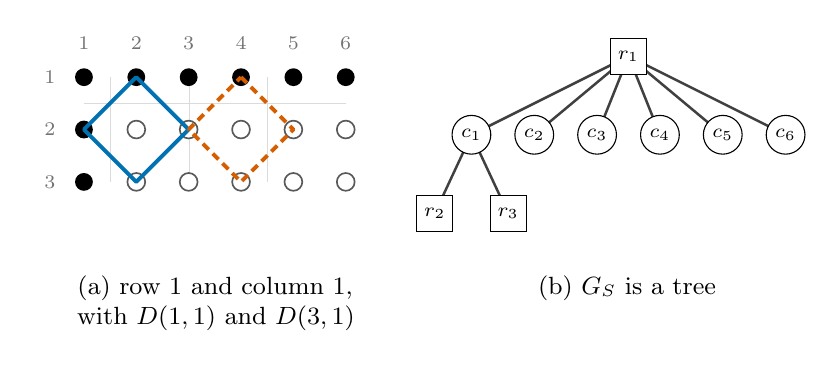
\begin{tikzpicture}[x=0.665cm,y=0.665cm,baseline=(current bounding box.north)]
  \draw[gridcol] (1,-1) grid (6,-3);
  \fill[black] (1,-1) circle (0.17);
  \fill[black] (2,-1) circle (0.17);
  \fill[black] (3,-1) circle (0.17);
  \fill[black] (4,-1) circle (0.17);
  \fill[black] (5,-1) circle (0.17);
  \fill[black] (6,-1) circle (0.17);
  \fill[black] (1,-2) circle (0.17);
  \filldraw[fill=white,draw=keptline,line width=0.6pt] (2,-2) circle (0.17);
  \filldraw[fill=white,draw=keptline,line width=0.6pt] (3,-2) circle (0.17);
  \filldraw[fill=white,draw=keptline,line width=0.6pt] (4,-2) circle (0.17);
  \filldraw[fill=white,draw=keptline,line width=0.6pt] (5,-2) circle (0.17);
  \filldraw[fill=white,draw=keptline,line width=0.6pt] (6,-2) circle (0.17);
  \fill[black] (1,-3) circle (0.17);
  \filldraw[fill=white,draw=keptline,line width=0.6pt] (2,-3) circle (0.17);
  \filldraw[fill=white,draw=keptline,line width=0.6pt] (3,-3) circle (0.17);
  \filldraw[fill=white,draw=keptline,line width=0.6pt] (4,-3) circle (0.17);
  \filldraw[fill=white,draw=keptline,line width=0.6pt] (5,-3) circle (0.17);
  \filldraw[fill=white,draw=keptline,line width=0.6pt] (6,-3) circle (0.17);
  \node[lab] at (1,-0.35) {1};
  \node[lab] at (2,-0.35) {2};
  \node[lab] at (3,-0.35) {3};
  \node[lab] at (4,-0.35) {4};
  \node[lab] at (5,-0.35) {5};
  \node[lab] at (6,-0.35) {6};
  \node[lab] at (0.35,-1) {1};
  \node[lab] at (0.35,-2) {2};
  \node[lab] at (0.35,-3) {3};
  \draw[draw=rectA,line width=1.4pt,line join=round] (2,-1) -- (3,-2) -- (2,-3) -- (1,-2) -- cycle;
  \draw[draw=rectB,line width=1.4pt,line join=round,dash pattern=on 3pt off 2pt] (4,-1) -- (5,-2) -- (4,-3) -- (3,-2) -- cycle;
  \node[capt,anchor=north,text width=4.52cm,align=center] at (3.5,-4.6) {(a) row 1 and column 1, with $D(1,1)$ and $D(3,1)$};
  \draw[draw=black!75,line width=0.9pt] (11.4,-0.6) -- (8.4,-2.1);
  \draw[draw=black!75,line width=0.9pt] (7.7,-3.6) -- (8.4,-2.1);
  \draw[draw=black!75,line width=0.9pt] (9.1,-3.6) -- (8.4,-2.1);
  \draw[draw=black!75,line width=0.9pt] (11.4,-0.6) -- (9.6,-2.1);
  \draw[draw=black!75,line width=0.9pt] (11.4,-0.6) -- (10.8,-2.1);
  \draw[draw=black!75,line width=0.9pt] (11.4,-0.6) -- (12.0,-2.1);
  \draw[draw=black!75,line width=0.9pt] (11.4,-0.6) -- (13.2,-2.1);
  \draw[draw=black!75,line width=0.9pt] (11.4,-0.6) -- (14.4,-2.1);
  \node[rowv] at (11.4,-0.6) {$r_{1}$};
  \node[colv] at (8.4,-2.1) {$c_{1}$};
  \node[colv] at (9.6,-2.1) {$c_{2}$};
  \node[colv] at (10.8,-2.1) {$c_{3}$};
  \node[colv] at (12.0,-2.1) {$c_{4}$};
  \node[colv] at (13.2,-2.1) {$c_{5}$};
  \node[colv] at (14.4,-2.1) {$c_{6}$};
  \node[rowv] at (7.7,-3.6) {$r_{2}$};
  \node[rowv] at (9.1,-3.6) {$r_{3}$};
  \node[capt,anchor=north,text width=4.32cm,align=center] at (11.4,-4.6) {(b) $G_S$ is a tree};
\end{tikzpicture}

\caption{The three-row construction for $m=6$. The diamond $D(1,1)$ (solid) shows only $(3,2)$
and $(2,3)$; the diamond $D(3,1)$ (dashed) shows 3 corners.}
\label{fig:three}
\end{figure}

\begin{proof}[Proof that $S$ is valid]
\emph{Axis-aligned rectangles.} In $G_S$ the vertex $r_1$ is joined to every column and $c_1$ is
also joined to $r_2$ and $r_3$ (Figure~\ref{fig:three}(b)). That is $m+3$ vertices, $m+2$ edges
and connected, so $G_S$ is a tree. A tree has no cycles at all, so by Lemma~\ref{lem:girth} no 2
axis-aligned rectangles look the same.

\emph{Tilted rectangles.} By Lemma~\ref{lem:tilted} they are the diamonds
$D(i,1)=\{(i,2),(i+1,1),(i+2,2),(i+1,3)\}$, $1\le i\le m-2$. Check each corner. The corner
$(i+1,1)$ is in row 1, so it is black. The corner $(i,2)$ is black only if $i=1$. The corners
$(i+2,2)$ and $(i+1,3)$ are in rows 2, 3 and columns at least 2, so they are white.

So for $i\ge2$ the diamond has 1 black corner and shows 3, and by
Lemma~\ref{lem:threecorners} nothing else shows the same 3 points. For $i=1$ the diamond shows
$\{(3,2),(2,3)\}$. Could another rectangle show exactly these 2 points? It would have both
points as corners. An axis-aligned rectangle with corners $(3,2)$ and $(2,3)$ has them as
opposite corners, so it is the square with corners $(2,2),(3,2),(2,3),(3,3)$, and $(2,2)$,
$(3,3)$ are white, so it shows 4 points. Every other diamond shows 3 points. So no other
rectangle shows $\{(3,2),(2,3)\}$.

Finally an axis-aligned rectangle and a diamond $D(i,1)$ with $i\ge2$ can only agree if both
show the same 3 points, which Lemma~\ref{lem:threecorners} rules out. So $S$ is valid.
\end{proof}

\begin{remark}
The same ``row 1 plus column 1'' blackout has $n+m-1$ points on any grid, and it is valid on
every grid up to $10\times10$ (checked by \texttt{verify\_narrow.py}). It is the maximum on 3
rows and on $4\times4$ and $4\times5$ (Section~\ref{sec:fourboundary}), but from $4\times6$ on
we can do 1 better.
\end{remark}

%======================================================================
\section{Four rows}\label{sec:four}

\subsection{The construction for $m\ge6$}

\begin{theorem}[Four-Row Theorem]\label{thm:fourrow}
For every $m\ge6$, the maximum blackout of the $4\times m$ grid is $m+4$.
\end{theorem}

The upper bound is the row bound, $m+\lfloor16/4\rfloor=m+4$. For the lower bound take
\[
S=\{(i,1):2\le i\le m-1\}\cup\{(m-1,2),(m,2),(1,3),(2,3),(1,4),(m,4)\},
\]
which has $(m-2)+6=m+4$ points.

\begin{figure}[htbp]
\centering
% generated by make_figures.py; width about 9.0 cm
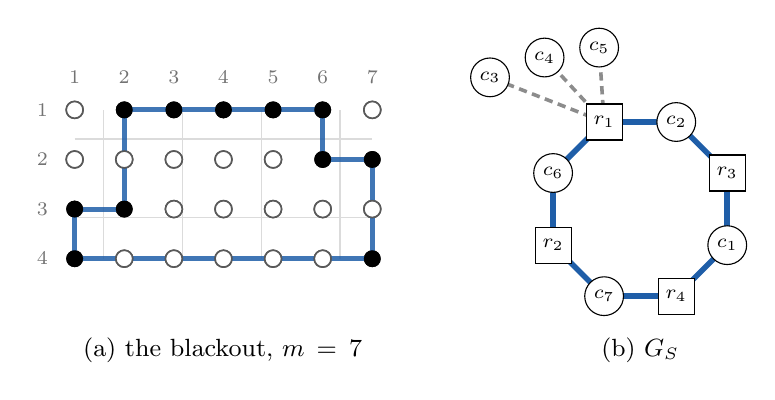
\begin{tikzpicture}[x=0.630cm,y=0.630cm,baseline=(current bounding box.north)]
  \draw[gridcol] (1,-1) grid (7,-4);
  \filldraw[fill=white,draw=keptline,line width=0.6pt] (1,-1) circle (0.17);
  \fill[black] (2,-1) circle (0.17);
  \fill[black] (3,-1) circle (0.17);
  \fill[black] (4,-1) circle (0.17);
  \fill[black] (5,-1) circle (0.17);
  \fill[black] (6,-1) circle (0.17);
  \filldraw[fill=white,draw=keptline,line width=0.6pt] (7,-1) circle (0.17);
  \filldraw[fill=white,draw=keptline,line width=0.6pt] (1,-2) circle (0.17);
  \filldraw[fill=white,draw=keptline,line width=0.6pt] (2,-2) circle (0.17);
  \filldraw[fill=white,draw=keptline,line width=0.6pt] (3,-2) circle (0.17);
  \filldraw[fill=white,draw=keptline,line width=0.6pt] (4,-2) circle (0.17);
  \filldraw[fill=white,draw=keptline,line width=0.6pt] (5,-2) circle (0.17);
  \fill[black] (6,-2) circle (0.17);
  \fill[black] (7,-2) circle (0.17);
  \fill[black] (1,-3) circle (0.17);
  \fill[black] (2,-3) circle (0.17);
  \filldraw[fill=white,draw=keptline,line width=0.6pt] (3,-3) circle (0.17);
  \filldraw[fill=white,draw=keptline,line width=0.6pt] (4,-3) circle (0.17);
  \filldraw[fill=white,draw=keptline,line width=0.6pt] (5,-3) circle (0.17);
  \filldraw[fill=white,draw=keptline,line width=0.6pt] (6,-3) circle (0.17);
  \filldraw[fill=white,draw=keptline,line width=0.6pt] (7,-3) circle (0.17);
  \fill[black] (1,-4) circle (0.17);
  \filldraw[fill=white,draw=keptline,line width=0.6pt] (2,-4) circle (0.17);
  \filldraw[fill=white,draw=keptline,line width=0.6pt] (3,-4) circle (0.17);
  \filldraw[fill=white,draw=keptline,line width=0.6pt] (4,-4) circle (0.17);
  \filldraw[fill=white,draw=keptline,line width=0.6pt] (5,-4) circle (0.17);
  \filldraw[fill=white,draw=keptline,line width=0.6pt] (6,-4) circle (0.17);
  \fill[black] (7,-4) circle (0.17);
  \node[lab] at (1,-0.35) {1};
  \node[lab] at (2,-0.35) {2};
  \node[lab] at (3,-0.35) {3};
  \node[lab] at (4,-0.35) {4};
  \node[lab] at (5,-0.35) {5};
  \node[lab] at (6,-0.35) {6};
  \node[lab] at (7,-0.35) {7};
  \node[lab] at (0.35,-1) {1};
  \node[lab] at (0.35,-2) {2};
  \node[lab] at (0.35,-3) {3};
  \node[lab] at (0.35,-4) {4};
  \draw[cyccol,line width=1.8pt,line join=round,opacity=0.85] (2,-1) -- (6,-1) -- (6,-2) -- (7,-2) -- (7,-4) -- (1,-4) -- (1,-3) -- (2,-3) -- cycle;
  \filldraw[fill=white,draw=keptline,line width=0.6pt] (1,-1) circle (0.17);
  \fill[black] (2,-1) circle (0.17);
  \fill[black] (3,-1) circle (0.17);
  \fill[black] (4,-1) circle (0.17);
  \fill[black] (5,-1) circle (0.17);
  \fill[black] (6,-1) circle (0.17);
  \filldraw[fill=white,draw=keptline,line width=0.6pt] (7,-1) circle (0.17);
  \filldraw[fill=white,draw=keptline,line width=0.6pt] (1,-2) circle (0.17);
  \filldraw[fill=white,draw=keptline,line width=0.6pt] (2,-2) circle (0.17);
  \filldraw[fill=white,draw=keptline,line width=0.6pt] (3,-2) circle (0.17);
  \filldraw[fill=white,draw=keptline,line width=0.6pt] (4,-2) circle (0.17);
  \filldraw[fill=white,draw=keptline,line width=0.6pt] (5,-2) circle (0.17);
  \fill[black] (6,-2) circle (0.17);
  \fill[black] (7,-2) circle (0.17);
  \fill[black] (1,-3) circle (0.17);
  \fill[black] (2,-3) circle (0.17);
  \filldraw[fill=white,draw=keptline,line width=0.6pt] (3,-3) circle (0.17);
  \filldraw[fill=white,draw=keptline,line width=0.6pt] (4,-3) circle (0.17);
  \filldraw[fill=white,draw=keptline,line width=0.6pt] (5,-3) circle (0.17);
  \filldraw[fill=white,draw=keptline,line width=0.6pt] (6,-3) circle (0.17);
  \filldraw[fill=white,draw=keptline,line width=0.6pt] (7,-3) circle (0.17);
  \fill[black] (1,-4) circle (0.17);
  \filldraw[fill=white,draw=keptline,line width=0.6pt] (2,-4) circle (0.17);
  \filldraw[fill=white,draw=keptline,line width=0.6pt] (3,-4) circle (0.17);
  \filldraw[fill=white,draw=keptline,line width=0.6pt] (4,-4) circle (0.17);
  \filldraw[fill=white,draw=keptline,line width=0.6pt] (5,-4) circle (0.17);
  \filldraw[fill=white,draw=keptline,line width=0.6pt] (6,-4) circle (0.17);
  \fill[black] (7,-4) circle (0.17);
  \node[capt,anchor=north,text width=4.41cm,align=center] at (4,-5.4) {(a) the blackout, $m=7$};
  \draw[draw=cyccol,line width=2pt] (14.155371111771444,-2.2729014785063293) -- (14.155371111771444,-3.7270985214936707);
  \draw[draw=cyccol,line width=2pt] (13.127098521493672,-4.755371111771445) -- (14.155371111771444,-3.7270985214936707);
  \draw[draw=cyccol,line width=2pt] (11.67290147850633,-1.2446288882285552) -- (13.127098521493672,-1.2446288882285552);
  \draw[draw=cyccol,line width=2pt] (14.155371111771444,-2.2729014785063293) -- (13.127098521493672,-1.2446288882285552);
  \draw[draw=pencol,line width=1.3pt,dash pattern=on 3pt off 2pt] (11.67290147850633,-1.2446288882285552) -- (9.372901478506328,-0.3446288882285552);
  \draw[draw=pencol,line width=1.3pt,dash pattern=on 3pt off 2pt] (11.67290147850633,-1.2446288882285552) -- (10.47290147850633,0.055371111771444825);
  \draw[draw=pencol,line width=1.3pt,dash pattern=on 3pt off 2pt] (11.67290147850633,-1.2446288882285552) -- (11.57290147850633,0.2553711117714448);
  \draw[draw=cyccol,line width=2pt] (11.67290147850633,-1.2446288882285552) -- (10.644628888228555,-2.2729014785063297);
  \draw[draw=cyccol,line width=2pt] (10.644628888228556,-3.7270985214936707) -- (10.644628888228555,-2.2729014785063297);
  \draw[draw=cyccol,line width=2pt] (10.644628888228556,-3.7270985214936707) -- (11.67290147850633,-4.755371111771445);
  \draw[draw=cyccol,line width=2pt] (13.127098521493672,-4.755371111771445) -- (11.67290147850633,-4.755371111771445);
  \node[rowv] at (11.67290147850633,-1.2446288882285552) {$r_{1}$};
  \node[colv] at (13.127098521493672,-1.2446288882285552) {$c_{2}$};
  \node[rowv] at (14.155371111771444,-2.2729014785063293) {$r_{3}$};
  \node[colv] at (14.155371111771444,-3.7270985214936707) {$c_{1}$};
  \node[rowv] at (13.127098521493672,-4.755371111771445) {$r_{4}$};
  \node[colv] at (11.67290147850633,-4.755371111771445) {$c_{7}$};
  \node[rowv] at (10.644628888228556,-3.7270985214936707) {$r_{2}$};
  \node[colv] at (10.644628888228555,-2.2729014785063297) {$c_{6}$};
  \node[colv] at (9.372901478506328,-0.3446288882285552) {$c_{3}$};
  \node[colv] at (10.47290147850633,0.055371111771444825) {$c_{4}$};
  \node[colv] at (11.57290147850633,0.2553711117714448) {$c_{5}$};
  \node[capt,anchor=north] at (12.4,-5.4) {(b) $G_S$};
\end{tikzpicture}

\caption{The four-row construction for $m=7$. The bold path in (a) turns only at black points
and alternates between rows and columns; it is the 8-cycle in (b). The columns $3,4,5$ hang off
$r_1$ (dashed).}
\label{fig:four}
\end{figure}

\begin{proof}[Proof that $S$ is valid]
\emph{Axis-aligned rectangles.} Only 4 columns have 2 black points: column 1 (rows 3, 4), column
2 (rows 1, 3), column $m-1$ (rows 1, 2) and column $m$ (rows 2, 4). Every other column is black
only in row 1. So $G_S$ is the 8-cycle
$r_1\,c_2\,r_3\,c_1\,r_4\,c_m\,r_2\,c_{m-1}$ with the columns $c_3,\ldots,c_{m-2}$ hanging off
$r_1$ (Figure~\ref{fig:four}). It has no 4-cycle and no 6-cycle, so Lemma~\ref{lem:girth}
handles the axis-aligned rectangles.

\emph{Tilted rectangles with at most 1 black corner.} These show 3 or 4 corners and are safe by
Lemma~\ref{lem:threecorners}. This covers $D(i,2)$, $C_i$ and $E_i$. For example, take
$D(i,2)=\{(i,3),(i+1,2),(i+2,3),(i+1,4)\}$. In rows 2 to 4 the black points are
$(m-1,2),(m,2),(1,3),(2,3),(1,4),(m,4)$. So $(i,3)$ is black only if $i\le2$, $(i+1,2)$ only
if $i=m-2$, and $(i+2,3)$ and $(i+1,4)$ are never black (since $3\le i+2$ and
$2\le i+1\le m-1$). Since $m\ge6$, $i\le2$ and $i=m-2$ can't both hold, so at most 1 corner is
black. For $C_i$ and $E_i$ the same kind of check shows that the only black corner is the one in
row 1.

\emph{The other tilted rectangles.} Checking each corner of each $D(i,1)$, $A_i$ and $B_i$ in
the same way gives the following list of the tilted rectangles that show at most 2 corners. Here
$F$ stands for $A$ (with $s=1$) or $B$ (with $s=2$).
\begin{center}\small
\begin{tabular}{lll}
\toprule
rectangle & which $i$ & corners shown\\
\midrule
$D(1,1)$ & & $(1,2),(3,2)$\\
$D(i,1)$ & $i=m-3,\,m-2$ & $(i,2),(i+1,3)$\\
$F_i$ & $i\in\{1,2\}$, $i\notin\{m-4,m-3\}$ & $(i+s,4),(i+3,2)$\\
$F_i$ & $i\in\{m-4,m-3\}$, $i\notin\{1,2\}$ & $(i,3),(i+s,4)$\\
$F_i$ & $i\in\{1,2\}\cap\{m-4,m-3\}$ & $(i+s,4)$\\
\bottomrule
\end{tabular}
\end{center}
The last line only happens when $m=6$ and $i=2$. As a sample check, take $A_1$, with corners $(1,3)$, $(2,4)$,
$(3,1)$ and $(4,2)$. The corners $(1,3)$ and $(3,1)$ are black, $(2,4)$ is white (row 4 is black only in columns 1
and $m$), and $(4,2)$ is white (row 2 is black only in columns $m-1,m$, and $4<m-1$). So $A_1$
shows $(2,4),(4,2)$, which is the third line with $s=1$. Figure~\ref{fig:fourtilted} shows the
cases for $m=7$. (The verification script also checks the whole construction against every
rectangle for each width from 6 to 40 and for 64, 100 and 128.)

We have to show that each presentation in the table belongs to only 1 rectangle.

\emph{Against each other.} The 2 shown points are in rows $\{2,2\}$ for $D(1,1)$, rows $\{2,3\}$
for the other diamonds, rows $\{2,4\}$ in line 3 and rows $\{3,4\}$ in line 4, so different
lines never agree. Within a line, the columns of the 2 points give $i$, and their horizontal
distance ($3-s$ in line 3 and $s$ in line 4) gives whether it is $A$ or $B$. The one-point
presentations in the last line are $(3,4)$ and $(4,4)$, which are different.

\emph{Against axis-aligned rectangles.}
\begin{itemize}[leftmargin=*,itemsep=1pt]
\item $D(1,1)$ shows $(1,2),(3,2)$, both in row 2. An axis-aligned rectangle showing exactly these
would use columns 1 and 3 and one more row in which both $(1,\cdot)$ and $(3,\cdot)$ are black.
Column 1 is black in rows 3, 4 and column 3 only in row 1, so there is no such row.
\item $D(i,1)$ with $i\ge m-3$ shows $(i,2),(i+1,3)$, which are in different rows and columns. The
only axis-aligned rectangle with these corners also has the corner $(i,3)$, which is white
because $i\ge m-3\ge3$. So that rectangle shows at least 3 points.
\item Line 3: the other axis-aligned corner $(i+s,2)$ is white, because $i+s\le4<m-1$.
\item Line 4: the other axis-aligned corner $(i,4)$ is white, because $3\le i\le m-3$.
\item The last line ($m=6$): an axis-aligned rectangle showing only $(z,4)$ with $z\in\{3,4\}$
would need another column $c$ and another row $r$ with $(c,4)$, $(z,r)$ and $(c,r)$ all black.
Then $c\in\{1,6\}$ (row 4) and $r=1$ (columns 3, 4 are black only in row 1), but $(1,1)$ and
$(6,1)$ are white.
\end{itemize}
Finally, no rectangle is fully black: an axis-aligned one would be a 4-cycle, and every tilted
one shows at least 1 point by the table and the paragraph before it. So $S$ is valid.
\end{proof}

\begin{figure}[htbp]
\centering
% generated by make_figures.py; width about 12.7 cm
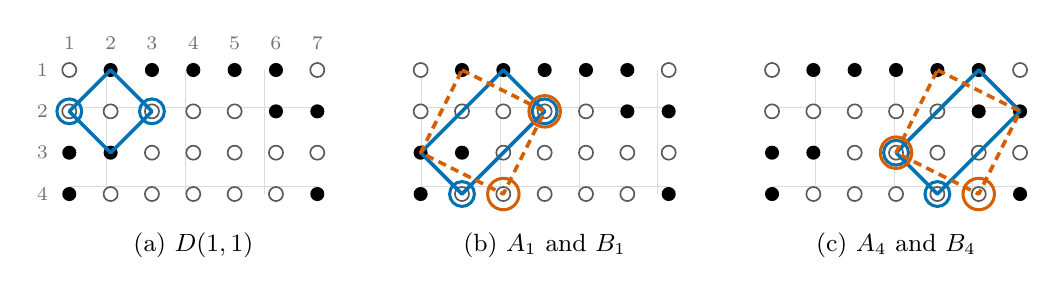
\begin{tikzpicture}[x=0.525cm,y=0.525cm,baseline=(current bounding box.north)]
  \draw[gridcol] (1.0,-1) grid (7.0,-4);
  \filldraw[fill=white,draw=keptline,line width=0.6pt] (1.0,-1) circle (0.17);
  \fill[black] (2.0,-1) circle (0.17);
  \fill[black] (3.0,-1) circle (0.17);
  \fill[black] (4.0,-1) circle (0.17);
  \fill[black] (5.0,-1) circle (0.17);
  \fill[black] (6.0,-1) circle (0.17);
  \filldraw[fill=white,draw=keptline,line width=0.6pt] (7.0,-1) circle (0.17);
  \filldraw[fill=white,draw=keptline,line width=0.6pt] (1.0,-2) circle (0.17);
  \filldraw[fill=white,draw=keptline,line width=0.6pt] (2.0,-2) circle (0.17);
  \filldraw[fill=white,draw=keptline,line width=0.6pt] (3.0,-2) circle (0.17);
  \filldraw[fill=white,draw=keptline,line width=0.6pt] (4.0,-2) circle (0.17);
  \filldraw[fill=white,draw=keptline,line width=0.6pt] (5.0,-2) circle (0.17);
  \fill[black] (6.0,-2) circle (0.17);
  \fill[black] (7.0,-2) circle (0.17);
  \fill[black] (1.0,-3) circle (0.17);
  \fill[black] (2.0,-3) circle (0.17);
  \filldraw[fill=white,draw=keptline,line width=0.6pt] (3.0,-3) circle (0.17);
  \filldraw[fill=white,draw=keptline,line width=0.6pt] (4.0,-3) circle (0.17);
  \filldraw[fill=white,draw=keptline,line width=0.6pt] (5.0,-3) circle (0.17);
  \filldraw[fill=white,draw=keptline,line width=0.6pt] (6.0,-3) circle (0.17);
  \filldraw[fill=white,draw=keptline,line width=0.6pt] (7.0,-3) circle (0.17);
  \fill[black] (1.0,-4) circle (0.17);
  \filldraw[fill=white,draw=keptline,line width=0.6pt] (2.0,-4) circle (0.17);
  \filldraw[fill=white,draw=keptline,line width=0.6pt] (3.0,-4) circle (0.17);
  \filldraw[fill=white,draw=keptline,line width=0.6pt] (4.0,-4) circle (0.17);
  \filldraw[fill=white,draw=keptline,line width=0.6pt] (5.0,-4) circle (0.17);
  \filldraw[fill=white,draw=keptline,line width=0.6pt] (6.0,-4) circle (0.17);
  \fill[black] (7.0,-4) circle (0.17);
  \node[lab] at (1.0,-0.35) {1};
  \node[lab] at (2.0,-0.35) {2};
  \node[lab] at (3.0,-0.35) {3};
  \node[lab] at (4.0,-0.35) {4};
  \node[lab] at (5.0,-0.35) {5};
  \node[lab] at (6.0,-0.35) {6};
  \node[lab] at (7.0,-0.35) {7};
  \node[lab] at (0.35,-1) {1};
  \node[lab] at (0.35,-2) {2};
  \node[lab] at (0.35,-3) {3};
  \node[lab] at (0.35,-4) {4};
  \draw[draw=rectA,line width=1.3pt,line join=round] (2.0,-1) -- (3.0,-2) -- (2.0,-3) -- (1.0,-2) -- cycle;
  \draw[rectA,line width=1.1pt] (1.0,-2) circle (0.3);
  \draw[rectA,line width=1.1pt] (3.0,-2) circle (0.3);
  \node[capt,anchor=north] at (4.0,-4.7) {(a) $D(1,1)$};
  \draw[gridcol] (9.5,-1) grid (15.5,-4);
  \filldraw[fill=white,draw=keptline,line width=0.6pt] (9.5,-1) circle (0.17);
  \fill[black] (10.5,-1) circle (0.17);
  \fill[black] (11.5,-1) circle (0.17);
  \fill[black] (12.5,-1) circle (0.17);
  \fill[black] (13.5,-1) circle (0.17);
  \fill[black] (14.5,-1) circle (0.17);
  \filldraw[fill=white,draw=keptline,line width=0.6pt] (15.5,-1) circle (0.17);
  \filldraw[fill=white,draw=keptline,line width=0.6pt] (9.5,-2) circle (0.17);
  \filldraw[fill=white,draw=keptline,line width=0.6pt] (10.5,-2) circle (0.17);
  \filldraw[fill=white,draw=keptline,line width=0.6pt] (11.5,-2) circle (0.17);
  \filldraw[fill=white,draw=keptline,line width=0.6pt] (12.5,-2) circle (0.17);
  \filldraw[fill=white,draw=keptline,line width=0.6pt] (13.5,-2) circle (0.17);
  \fill[black] (14.5,-2) circle (0.17);
  \fill[black] (15.5,-2) circle (0.17);
  \fill[black] (9.5,-3) circle (0.17);
  \fill[black] (10.5,-3) circle (0.17);
  \filldraw[fill=white,draw=keptline,line width=0.6pt] (11.5,-3) circle (0.17);
  \filldraw[fill=white,draw=keptline,line width=0.6pt] (12.5,-3) circle (0.17);
  \filldraw[fill=white,draw=keptline,line width=0.6pt] (13.5,-3) circle (0.17);
  \filldraw[fill=white,draw=keptline,line width=0.6pt] (14.5,-3) circle (0.17);
  \filldraw[fill=white,draw=keptline,line width=0.6pt] (15.5,-3) circle (0.17);
  \fill[black] (9.5,-4) circle (0.17);
  \filldraw[fill=white,draw=keptline,line width=0.6pt] (10.5,-4) circle (0.17);
  \filldraw[fill=white,draw=keptline,line width=0.6pt] (11.5,-4) circle (0.17);
  \filldraw[fill=white,draw=keptline,line width=0.6pt] (12.5,-4) circle (0.17);
  \filldraw[fill=white,draw=keptline,line width=0.6pt] (13.5,-4) circle (0.17);
  \filldraw[fill=white,draw=keptline,line width=0.6pt] (14.5,-4) circle (0.17);
  \fill[black] (15.5,-4) circle (0.17);
  \draw[draw=rectA,line width=1.3pt,line join=round] (11.5,-1) -- (12.5,-2) -- (10.5,-4) -- (9.5,-3) -- cycle;
  \draw[rectA,line width=1.1pt] (10.5,-4) circle (0.3);
  \draw[rectA,line width=1.1pt] (12.5,-2) circle (0.3);
  \draw[draw=rectB,line width=1.3pt,line join=round,dash pattern=on 3pt off 2pt] (10.5,-1) -- (12.5,-2) -- (11.5,-4) -- (9.5,-3) -- cycle;
  \draw[rectB,line width=1.1pt] (11.5,-4) circle (0.38);
  \draw[rectB,line width=1.1pt] (12.5,-2) circle (0.38);
  \node[capt,anchor=north] at (12.5,-4.7) {(b) $A_1$ and $B_1$};
  \draw[gridcol] (18.0,-1) grid (24.0,-4);
  \filldraw[fill=white,draw=keptline,line width=0.6pt] (18.0,-1) circle (0.17);
  \fill[black] (19.0,-1) circle (0.17);
  \fill[black] (20.0,-1) circle (0.17);
  \fill[black] (21.0,-1) circle (0.17);
  \fill[black] (22.0,-1) circle (0.17);
  \fill[black] (23.0,-1) circle (0.17);
  \filldraw[fill=white,draw=keptline,line width=0.6pt] (24.0,-1) circle (0.17);
  \filldraw[fill=white,draw=keptline,line width=0.6pt] (18.0,-2) circle (0.17);
  \filldraw[fill=white,draw=keptline,line width=0.6pt] (19.0,-2) circle (0.17);
  \filldraw[fill=white,draw=keptline,line width=0.6pt] (20.0,-2) circle (0.17);
  \filldraw[fill=white,draw=keptline,line width=0.6pt] (21.0,-2) circle (0.17);
  \filldraw[fill=white,draw=keptline,line width=0.6pt] (22.0,-2) circle (0.17);
  \fill[black] (23.0,-2) circle (0.17);
  \fill[black] (24.0,-2) circle (0.17);
  \fill[black] (18.0,-3) circle (0.17);
  \fill[black] (19.0,-3) circle (0.17);
  \filldraw[fill=white,draw=keptline,line width=0.6pt] (20.0,-3) circle (0.17);
  \filldraw[fill=white,draw=keptline,line width=0.6pt] (21.0,-3) circle (0.17);
  \filldraw[fill=white,draw=keptline,line width=0.6pt] (22.0,-3) circle (0.17);
  \filldraw[fill=white,draw=keptline,line width=0.6pt] (23.0,-3) circle (0.17);
  \filldraw[fill=white,draw=keptline,line width=0.6pt] (24.0,-3) circle (0.17);
  \fill[black] (18.0,-4) circle (0.17);
  \filldraw[fill=white,draw=keptline,line width=0.6pt] (19.0,-4) circle (0.17);
  \filldraw[fill=white,draw=keptline,line width=0.6pt] (20.0,-4) circle (0.17);
  \filldraw[fill=white,draw=keptline,line width=0.6pt] (21.0,-4) circle (0.17);
  \filldraw[fill=white,draw=keptline,line width=0.6pt] (22.0,-4) circle (0.17);
  \filldraw[fill=white,draw=keptline,line width=0.6pt] (23.0,-4) circle (0.17);
  \fill[black] (24.0,-4) circle (0.17);
  \draw[draw=rectA,line width=1.3pt,line join=round] (23.0,-1) -- (24.0,-2) -- (22.0,-4) -- (21.0,-3) -- cycle;
  \draw[rectA,line width=1.1pt] (21.0,-3) circle (0.3);
  \draw[rectA,line width=1.1pt] (22.0,-4) circle (0.3);
  \draw[draw=rectB,line width=1.3pt,line join=round,dash pattern=on 3pt off 2pt] (22.0,-1) -- (24.0,-2) -- (23.0,-4) -- (21.0,-3) -- cycle;
  \draw[rectB,line width=1.1pt] (21.0,-3) circle (0.38);
  \draw[rectB,line width=1.1pt] (23.0,-4) circle (0.38);
  \node[capt,anchor=north] at (21.0,-4.7) {(c) $A_4$ and $B_4$};
\end{tikzpicture}

\caption{Tilted rectangles with 2 black corners in the construction for $m=7$, with the shown
corners ringed. Each pair of shown points belongs to no other rectangle.}
\label{fig:fourtilted}
\end{figure}

\subsection{Widths 4 and 5}\label{sec:fourboundary}

On $4\times4$ and $4\times5$ the row bound says $m+4$, but the answer is $m+3$. To prove it we
first narrow down what a blackout of $m+4$ points would have to look like.

\begin{lemma}[equality in the row bound]\label{lem:fourclassification}
Let $m\ge4$. If a valid blackout of the $4\times m$ grid has $m+4$ points, then every column is
non-empty, exactly 4 columns have 2 black points and the others have 1, and the graph $H$ of
Section~\ref{sec:rowbound} is a 4-cycle on the 4 rows.
\end{lemma}

\begin{proof}
By Lemma~\ref{lem:H}, $m+4=|S|=t+e(H)$ with $t\le m$ and $e(H)\le4$, so $t=m$ (every column is
non-empty) and $e(H)=4$. Recall $e(H)=\sum_i(|B_i|-1)$.

A column black in all 4 rows gives 3 edges, and then every other column has at most 1 black
point (2 would share 2 rows with it, a 4-cycle), so $e(H)=3$. A column black in 3 rows gives 2
edges. Any other column with 2 or more black points can share at most 1 row with it, so it is a
pair made of the fourth row and 1 of the 3. There is at most 1 such column: 2 with the same pair
give a 4-cycle, and 2 with different pairs give a 6-cycle. So $e(H)\le2+1=3$. Hence every column
has 1 or 2 black points, and exactly 4 columns have 2.

These 4 columns give 4 edges of $H$, with no repeats and no triangle. A graph on 4 vertices with
4 edges misses 2 of the 6 possible edges. If the 2 missing edges shared a vertex $v$, the other 3
vertices would form a triangle. So the missing edges don't touch, and what is left is a 4-cycle.
\end{proof}

\begin{figure}[htbp]
\centering
% generated by make_figures.py; width about 12.1 cm
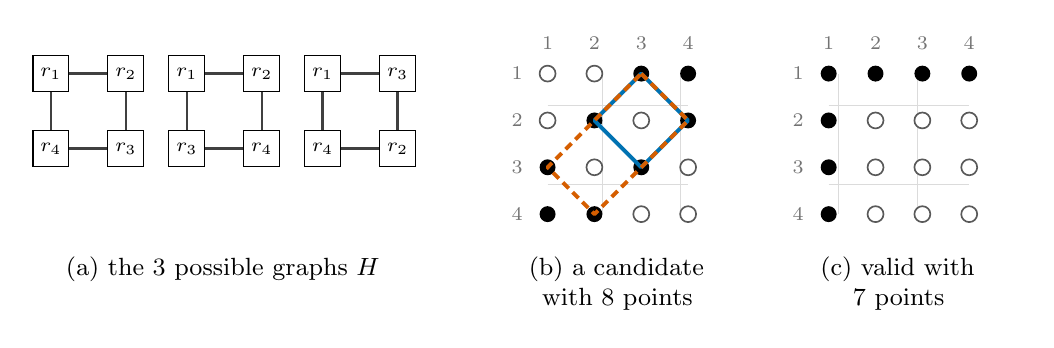
\begin{tikzpicture}[x=0.595cm,y=0.595cm,baseline=(current bounding box.north)]
  \draw[draw=black!75,line width=0.9pt] (0.0,-1.0) -- (1.6,-1.0);
  \draw[draw=black!75,line width=0.9pt] (1.6,-1.0) -- (1.6,-2.6);
  \draw[draw=black!75,line width=0.9pt] (1.6,-2.6) -- (0.0,-2.6);
  \draw[draw=black!75,line width=0.9pt] (0.0,-2.6) -- (0.0,-1.0);
  \node[rowv] at (0.0,-1.0) {$r_{1}$};
  \node[rowv] at (1.6,-1.0) {$r_{2}$};
  \node[rowv] at (1.6,-2.6) {$r_{3}$};
  \node[rowv] at (0.0,-2.6) {$r_{4}$};
  \draw[draw=black!75,line width=0.9pt] (2.9,-1.0) -- (4.5,-1.0);
  \draw[draw=black!75,line width=0.9pt] (4.5,-1.0) -- (4.5,-2.6);
  \draw[draw=black!75,line width=0.9pt] (4.5,-2.6) -- (2.9,-2.6);
  \draw[draw=black!75,line width=0.9pt] (2.9,-2.6) -- (2.9,-1.0);
  \node[rowv] at (2.9,-1.0) {$r_{1}$};
  \node[rowv] at (4.5,-1.0) {$r_{2}$};
  \node[rowv] at (4.5,-2.6) {$r_{4}$};
  \node[rowv] at (2.9,-2.6) {$r_{3}$};
  \draw[draw=black!75,line width=0.9pt] (5.8,-1.0) -- (7.4,-1.0);
  \draw[draw=black!75,line width=0.9pt] (7.4,-1.0) -- (7.4,-2.6);
  \draw[draw=black!75,line width=0.9pt] (7.4,-2.6) -- (5.8,-2.6);
  \draw[draw=black!75,line width=0.9pt] (5.8,-2.6) -- (5.8,-1.0);
  \node[rowv] at (5.8,-1.0) {$r_{1}$};
  \node[rowv] at (7.4,-1.0) {$r_{3}$};
  \node[rowv] at (7.4,-2.6) {$r_{2}$};
  \node[rowv] at (5.8,-2.6) {$r_{4}$};
  \node[capt,anchor=north,text width=4.76cm,align=center] at (3.7,-4.7) {(a) the 3 possible graphs $H$};
  \draw[gridcol] (10.6,-1) grid (13.6,-4);
  \filldraw[fill=white,draw=keptline,line width=0.6pt] (10.6,-1) circle (0.17);
  \filldraw[fill=white,draw=keptline,line width=0.6pt] (11.6,-1) circle (0.17);
  \fill[black] (12.6,-1) circle (0.17);
  \fill[black] (13.6,-1) circle (0.17);
  \filldraw[fill=white,draw=keptline,line width=0.6pt] (10.6,-2) circle (0.17);
  \fill[black] (11.6,-2) circle (0.17);
  \filldraw[fill=white,draw=keptline,line width=0.6pt] (12.6,-2) circle (0.17);
  \fill[black] (13.6,-2) circle (0.17);
  \fill[black] (10.6,-3) circle (0.17);
  \filldraw[fill=white,draw=keptline,line width=0.6pt] (11.6,-3) circle (0.17);
  \fill[black] (12.6,-3) circle (0.17);
  \filldraw[fill=white,draw=keptline,line width=0.6pt] (13.6,-3) circle (0.17);
  \fill[black] (10.6,-4) circle (0.17);
  \fill[black] (11.6,-4) circle (0.17);
  \filldraw[fill=white,draw=keptline,line width=0.6pt] (12.6,-4) circle (0.17);
  \filldraw[fill=white,draw=keptline,line width=0.6pt] (13.6,-4) circle (0.17);
  \node[lab] at (10.6,-0.35) {1};
  \node[lab] at (11.6,-0.35) {2};
  \node[lab] at (12.6,-0.35) {3};
  \node[lab] at (13.6,-0.35) {4};
  \node[lab] at (9.95,-1) {1};
  \node[lab] at (9.95,-2) {2};
  \node[lab] at (9.95,-3) {3};
  \node[lab] at (9.95,-4) {4};
  \draw[draw=rectA,line width=1.4pt,line join=round] (12.6,-1) -- (13.6,-2) -- (12.6,-3) -- (11.6,-2) -- cycle;
  \draw[draw=rectB,line width=1.4pt,line join=round,dash pattern=on 3pt off 2pt] (12.6,-1) -- (13.6,-2) -- (11.6,-4) -- (10.6,-3) -- cycle;
  \node[capt,anchor=north,text width=2.98cm,align=center] at (12.1,-4.7) {(b) a candidate with 8 points};
  \draw[gridcol] (16.6,-1) grid (19.6,-4);
  \fill[black] (16.6,-1) circle (0.17);
  \fill[black] (17.6,-1) circle (0.17);
  \fill[black] (18.6,-1) circle (0.17);
  \fill[black] (19.6,-1) circle (0.17);
  \fill[black] (16.6,-2) circle (0.17);
  \filldraw[fill=white,draw=keptline,line width=0.6pt] (17.6,-2) circle (0.17);
  \filldraw[fill=white,draw=keptline,line width=0.6pt] (18.6,-2) circle (0.17);
  \filldraw[fill=white,draw=keptline,line width=0.6pt] (19.6,-2) circle (0.17);
  \fill[black] (16.6,-3) circle (0.17);
  \filldraw[fill=white,draw=keptline,line width=0.6pt] (17.6,-3) circle (0.17);
  \filldraw[fill=white,draw=keptline,line width=0.6pt] (18.6,-3) circle (0.17);
  \filldraw[fill=white,draw=keptline,line width=0.6pt] (19.6,-3) circle (0.17);
  \fill[black] (16.6,-4) circle (0.17);
  \filldraw[fill=white,draw=keptline,line width=0.6pt] (17.6,-4) circle (0.17);
  \filldraw[fill=white,draw=keptline,line width=0.6pt] (18.6,-4) circle (0.17);
  \filldraw[fill=white,draw=keptline,line width=0.6pt] (19.6,-4) circle (0.17);
  \node[lab] at (16.6,-0.35) {1};
  \node[lab] at (17.6,-0.35) {2};
  \node[lab] at (18.6,-0.35) {3};
  \node[lab] at (19.6,-0.35) {4};
  \node[lab] at (15.95,-1) {1};
  \node[lab] at (15.95,-2) {2};
  \node[lab] at (15.95,-3) {3};
  \node[lab] at (15.95,-4) {4};
  \node[capt,anchor=north,text width=2.98cm,align=center] at (18.1,-4.7) {(c) valid with 7 points};
\end{tikzpicture}

\caption{(a) The 3 possible 4-cycles $H$ on the rows. (b) One of the 72 candidates on the
$4\times4$ grid. The tilted rectangles $D(2,1)$ (solid) and $A_1$ (dashed) are both completely
black, so both have empty presentations. (c) Row 1 plus column 1: valid, with 7 points.}
\label{fig:fourcases}
\end{figure}

\begin{corollary}[computer-assisted]\label{cor:fourboundary}
The maximum blackout is 7 on the $4\times4$ grid and 8 on the $4\times5$ grid.
\end{corollary}

\begin{proof}
The row bound gives at most $m+4$, and Lemma~\ref{lem:fourclassification} says what a blackout
of size $m+4$ looks like. So we can list all of them: choose 1 of the 3 four-cycles on the rows
(Figure~\ref{fig:fourcases}(a)), choose the 4 columns with 2 black points, match the 4 edges of
the cycle to those 4 columns, and choose 1 black row for each remaining column. That is
\[
3\cdot\binom m4\cdot4!\cdot4^{m-4}
\]
candidates, which is 72 for $m=4$ and 1,440 for $m=5$. The script \texttt{verify\_narrow.py}
checks every candidate against all rectangles, and every one of them has 2 rectangles with the
same presentation. Figure~\ref{fig:fourcases}(b) shows one. So the maximum is at most $m+3$.
Row 1 plus column 1 has $m+3$ points and the script checks that it is valid on both grids, so the
maximum is $m+3$.
\end{proof}

In Figure~\ref{fig:fourcases}(b) the axis-aligned rectangles are fine (the graph has no short
cycle), and the trouble comes from 2 tilted rectangles that are both completely hidden. This is
Remark~\ref{rem:empty} at work. Of the 72 candidates on $4\times4$, the first collision the
script finds involves only tilted rectangles in 9 cases and 1 axis-aligned rectangle in the other
63; on $4\times5$ the split is 118 and 1,322.

%======================================================================
\section{The $5\times5$ grid}\label{sec:five}

The $5\times5$ grid is the first square where $n+m-1$ is not the answer. It is also the smallest
grid with both sides at least 5. The row bound only gives $5+\lfloor25/4\rfloor=11$ here. The
answer is 10, and the proof is a counting argument on the graph $G_S$.

\subsection{The upper bound}

On a $5\times5$ grid the graph $G_S$ has only $10$ vertices. Lemma~\ref{lem:girth} rules out
cycles of length 4 and 6, and $G_S$ is bipartite, so every cycle has length at least 8. On 10
vertices there is room for 1 such cycle but not for 2 that overlap, and 2 that don't overlap
need at least 16 vertices. So $G_S$ can't have more edges than vertices.

\begin{lemma}[few edges without short cycles]\label{lem:tenvertices}
Let $G$ be a bipartite graph with $v\le10$ vertices and no cycle of length 4 or 6. Then $G$ has
at most $v$ edges. If it has exactly $v$ edges, then $G$ is connected and has exactly 1 cycle, of
length 8 or 10.
\end{lemma}

\begin{figure}[htbp]
\centering
% generated by make_figures.py; width about 6.5 cm
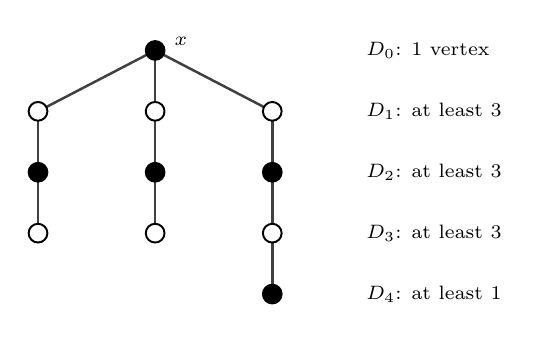
\begin{tikzpicture}[x=0.595cm,y=0.595cm,baseline=(current bounding box.north)]
  \draw[black!75,line width=0.9pt] (4.0,-1.0) -- (1.5,-2.3);
  \draw[black!75,line width=0.9pt] (4.0,-1.0) -- (4.0,-2.3);
  \draw[black!75,line width=0.9pt] (4.0,-1.0) -- (6.5,-2.3);
  \draw[black!75,line width=0.9pt] (1.5,-2.3) -- (1.5,-3.6);
  \draw[black!75,line width=0.9pt] (4.0,-2.3) -- (4.0,-3.6);
  \draw[black!75,line width=0.9pt] (6.5,-2.3) -- (6.5,-3.6);
  \draw[black!75,line width=0.9pt] (1.5,-3.6) -- (1.5,-4.9);
  \draw[black!75,line width=0.9pt] (4.0,-3.6) -- (4.0,-4.9);
  \draw[black!75,line width=0.9pt] (6.5,-3.6) -- (6.5,-4.9);
  \draw[black!75,line width=0.9pt] (6.5,-4.9) -- (6.5,-6.2);
  \filldraw[fill=black,draw=black,line width=0.7pt] (4.0,-1.0) circle (0.2);
  \filldraw[fill=white,draw=black,line width=0.7pt] (1.5,-2.3) circle (0.2);
  \filldraw[fill=white,draw=black,line width=0.7pt] (4.0,-2.3) circle (0.2);
  \filldraw[fill=white,draw=black,line width=0.7pt] (6.5,-2.3) circle (0.2);
  \filldraw[fill=black,draw=black,line width=0.7pt] (1.5,-3.6) circle (0.2);
  \filldraw[fill=black,draw=black,line width=0.7pt] (4.0,-3.6) circle (0.2);
  \filldraw[fill=black,draw=black,line width=0.7pt] (6.5,-3.6) circle (0.2);
  \filldraw[fill=white,draw=black,line width=0.7pt] (1.5,-4.9) circle (0.2);
  \filldraw[fill=white,draw=black,line width=0.7pt] (4.0,-4.9) circle (0.2);
  \filldraw[fill=white,draw=black,line width=0.7pt] (6.5,-4.9) circle (0.2);
  \filldraw[fill=black,draw=black,line width=0.7pt] (6.5,-6.2) circle (0.2);
  \node[tiny] at (4.55,-0.8) {$x$};
  \node[tiny,anchor=west] at (8.3,-1.0) {$D_0$: 1 vertex};
  \node[tiny,anchor=west] at (8.3,-2.3) {$D_1$: at least 3};
  \node[tiny,anchor=west] at (8.3,-3.6) {$D_2$: at least 3};
  \node[tiny,anchor=west] at (8.3,-4.9) {$D_3$: at least 3};
  \node[tiny,anchor=west] at (8.3,-6.2) {$D_4$: at least 1};
\end{tikzpicture}

\caption{The count in Step 1. Around a vertex $x$ of degree at least 3, the vertices at distance
at most 3 form a tree, so there are at least $1+3+3+3$ of them, and each vertex at distance 3
leads on to a vertex at distance 4. Black and white show the 2 sides of the bipartite graph.}
\label{fig:bfs}
\end{figure}

\begin{proof}
Since $G$ is bipartite, every cycle has even length, so every cycle has length at least 8.

\emph{Step 1: no connected piece of $G$ has more edges than vertices.} Suppose a piece $G'$ does.
Remove a vertex of degree 1 from $G'$, together with its edge, and repeat until there are none.
Each step removes 1 vertex and 1 edge, so what is left, $H$, still has more edges than vertices.
In particular $H$ isn't empty and every vertex of $H$ has degree at least 2. If every degree
were exactly 2, $H$ would have as many edges as vertices, so some vertex $x$ has degree at least
3.

Let $D_k$ be the set of vertices of $H$ at distance $k$ from $x$. Two different paths from $x$ to
the same vertex, each of length at most 3, would together contain a cycle of length at most 6,
which is impossible. So for $k=1,2,3$ each vertex of $D_k$ has exactly 1 neighbour in $D_{k-1}$,
its \emph{parent}. It has no neighbour in $D_k$ itself, because $D_k$ is on one side of the
bipartite graph. Its degree is at least 2, so it has a neighbour in $D_{k+1}$. Two different
vertices of $D_k$ (with $k\le2$) can't share such a neighbour, since that neighbour would have 2
parents. So $|D_1|\ge3$, $|D_2|\ge|D_1|\ge3$, $|D_3|\ge|D_2|\ge3$ and $|D_4|\ge1$
(Figure~\ref{fig:bfs}). That is at least $1+3+3+3+1=11$ vertices, but $v\le10$. This
contradiction proves Step 1.

\emph{Step 2: equality.} By Step 1 each piece has at most as many edges as vertices, so $G$ has
at most $v$ edges. If it has exactly $v$, each piece has exactly as many edges as vertices, and a
connected graph like that has exactly 1 cycle. Two pieces would mean 2 separate cycles of length
at least 8, which needs 16 vertices. So $G$ is connected, and its 1 cycle has even length between
8 and 10.
\end{proof}

\begin{theorem}[the $5\times5$ grid]\label{thm:fivefive}
The maximum blackout of the $5\times5$ grid is 10. For every maximum blackout $S$, the graph
$G_S$ is connected with exactly 1 cycle, of length 8 or 10. By computer, there are exactly 8
maximum blackouts, they are the 8 images of Figure~\ref{fig:fivefive}(a) under the symmetries of
the square, and each graph is an 8-cycle with 2 pendant edges.
\end{theorem}

\begin{proof}
\emph{Upper bound.} If $S$ is valid, $G_S$ has no 4-cycle or 6-cycle (Lemma~\ref{lem:girth}, with
$m=5\ge3$). It is bipartite with 10 vertices and $|S|$ edges, so Lemma~\ref{lem:tenvertices}
gives $|S|\le10$, and if $|S|=10$ it gives the structure in the statement.

\emph{Lower bound.} The blackout in Figure~\ref{fig:fivefive}(a) has 10 points. Its graph is an
8-cycle with 2 pendant edges, so Lemma~\ref{lem:girth} handles the 100 axis-aligned rectangles.
The script checks all 130 presentations directly and finds them all different.

\emph{The count.} A maximum blackout has a graph with 10 edges and no 4- or 6-cycle. The script
lists all 44,640 such sets of 10 points (adding points one at a time and only keeping a point if
no short cycle appears), and checks each one against all 130 rectangles. Exactly 8 are valid,
and they are the 8 images in Figure~\ref{fig:orbit}. The count of 8 had been found earlier, in a
completely separate way, by the hitting set program and by checking every blackout straight from
the definition (Section~\ref{sec:computations}).
\end{proof}

\begin{figure}[htbp]
\centering
% generated by make_figures.py; width about 8.7 cm
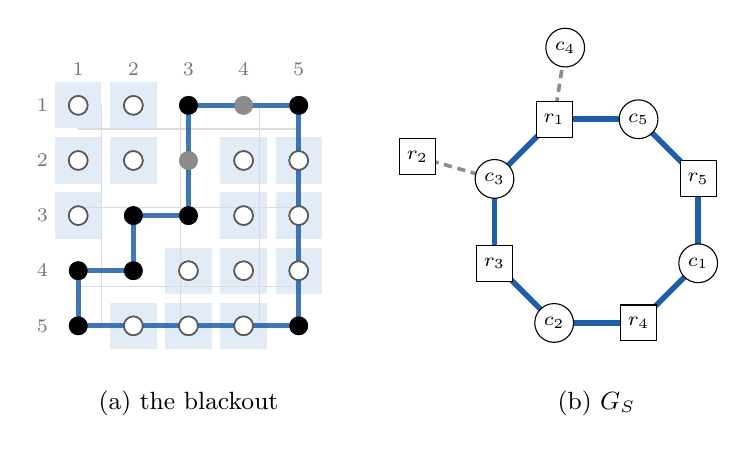
\begin{tikzpicture}[x=0.700cm,y=0.700cm,baseline=(current bounding box.north)]
  \fill[keptcol] (3.58,-4.42) rectangle (4.42,-3.58);
  \fill[keptcol] (0.5800000000000001,-2.42) rectangle (1.42,-1.58);
  \fill[keptcol] (2.58,-4.42) rectangle (3.42,-3.58);
  \fill[keptcol] (1.58,-1.42) rectangle (2.42,-0.5800000000000001);
  \fill[keptcol] (3.58,-3.42) rectangle (4.42,-2.58);
  \fill[keptcol] (4.58,-4.42) rectangle (5.42,-3.58);
  \fill[keptcol] (0.5800000000000001,-1.42) rectangle (1.42,-0.5800000000000001);
  \fill[keptcol] (3.58,-2.42) rectangle (4.42,-1.58);
  \fill[keptcol] (3.58,-5.42) rectangle (4.42,-4.58);
  \fill[keptcol] (1.58,-2.42) rectangle (2.42,-1.58);
  \fill[keptcol] (4.58,-3.42) rectangle (5.42,-2.58);
  \fill[keptcol] (1.58,-5.42) rectangle (2.42,-4.58);
  \fill[keptcol] (0.5800000000000001,-3.42) rectangle (1.42,-2.58);
  \fill[keptcol] (2.58,-5.42) rectangle (3.42,-4.58);
  \fill[keptcol] (4.58,-2.42) rectangle (5.42,-1.58);
  \draw[gridcol] (1,-1) grid (5,-5);
  \filldraw[fill=white,draw=keptline,line width=0.6pt] (1,-1) circle (0.17);
  \filldraw[fill=white,draw=keptline,line width=0.6pt] (2,-1) circle (0.17);
  \fill[black] (3,-1) circle (0.17);
  \fill[pencol] (4,-1) circle (0.17);
  \fill[black] (5,-1) circle (0.17);
  \filldraw[fill=white,draw=keptline,line width=0.6pt] (1,-2) circle (0.17);
  \filldraw[fill=white,draw=keptline,line width=0.6pt] (2,-2) circle (0.17);
  \fill[pencol] (3,-2) circle (0.17);
  \filldraw[fill=white,draw=keptline,line width=0.6pt] (4,-2) circle (0.17);
  \filldraw[fill=white,draw=keptline,line width=0.6pt] (5,-2) circle (0.17);
  \filldraw[fill=white,draw=keptline,line width=0.6pt] (1,-3) circle (0.17);
  \fill[black] (2,-3) circle (0.17);
  \fill[black] (3,-3) circle (0.17);
  \filldraw[fill=white,draw=keptline,line width=0.6pt] (4,-3) circle (0.17);
  \filldraw[fill=white,draw=keptline,line width=0.6pt] (5,-3) circle (0.17);
  \fill[black] (1,-4) circle (0.17);
  \fill[black] (2,-4) circle (0.17);
  \filldraw[fill=white,draw=keptline,line width=0.6pt] (3,-4) circle (0.17);
  \filldraw[fill=white,draw=keptline,line width=0.6pt] (4,-4) circle (0.17);
  \filldraw[fill=white,draw=keptline,line width=0.6pt] (5,-4) circle (0.17);
  \fill[black] (1,-5) circle (0.17);
  \filldraw[fill=white,draw=keptline,line width=0.6pt] (2,-5) circle (0.17);
  \filldraw[fill=white,draw=keptline,line width=0.6pt] (3,-5) circle (0.17);
  \filldraw[fill=white,draw=keptline,line width=0.6pt] (4,-5) circle (0.17);
  \fill[black] (5,-5) circle (0.17);
  \node[lab] at (1,-0.35) {1};
  \node[lab] at (2,-0.35) {2};
  \node[lab] at (3,-0.35) {3};
  \node[lab] at (4,-0.35) {4};
  \node[lab] at (5,-0.35) {5};
  \node[lab] at (0.35,-1) {1};
  \node[lab] at (0.35,-2) {2};
  \node[lab] at (0.35,-3) {3};
  \node[lab] at (0.35,-4) {4};
  \node[lab] at (0.35,-5) {5};
  \draw[cyccol,line width=1.8pt,line join=round,opacity=0.85] (3,-1) -- (5,-1) -- (5,-5) -- (1,-5) -- (1,-4) -- (2,-4) -- (2,-3) -- (3,-3) -- cycle;
  \filldraw[fill=white,draw=keptline,line width=0.6pt] (1,-1) circle (0.17);
  \filldraw[fill=white,draw=keptline,line width=0.6pt] (2,-1) circle (0.17);
  \fill[black] (3,-1) circle (0.17);
  \fill[pencol] (4,-1) circle (0.17);
  \fill[black] (5,-1) circle (0.17);
  \filldraw[fill=white,draw=keptline,line width=0.6pt] (1,-2) circle (0.17);
  \filldraw[fill=white,draw=keptline,line width=0.6pt] (2,-2) circle (0.17);
  \fill[pencol] (3,-2) circle (0.17);
  \filldraw[fill=white,draw=keptline,line width=0.6pt] (4,-2) circle (0.17);
  \filldraw[fill=white,draw=keptline,line width=0.6pt] (5,-2) circle (0.17);
  \filldraw[fill=white,draw=keptline,line width=0.6pt] (1,-3) circle (0.17);
  \fill[black] (2,-3) circle (0.17);
  \fill[black] (3,-3) circle (0.17);
  \filldraw[fill=white,draw=keptline,line width=0.6pt] (4,-3) circle (0.17);
  \filldraw[fill=white,draw=keptline,line width=0.6pt] (5,-3) circle (0.17);
  \fill[black] (1,-4) circle (0.17);
  \fill[black] (2,-4) circle (0.17);
  \filldraw[fill=white,draw=keptline,line width=0.6pt] (3,-4) circle (0.17);
  \filldraw[fill=white,draw=keptline,line width=0.6pt] (4,-4) circle (0.17);
  \filldraw[fill=white,draw=keptline,line width=0.6pt] (5,-4) circle (0.17);
  \fill[black] (1,-5) circle (0.17);
  \filldraw[fill=white,draw=keptline,line width=0.6pt] (2,-5) circle (0.17);
  \filldraw[fill=white,draw=keptline,line width=0.6pt] (3,-5) circle (0.17);
  \filldraw[fill=white,draw=keptline,line width=0.6pt] (4,-5) circle (0.17);
  \fill[black] (5,-5) circle (0.17);
  \node[capt,anchor=north] at (3,-6.0) {(a) the blackout};
  \draw[draw=cyccol,line width=2pt] (11.16536686473018,-4.947759065022574) -- (12.247759065022574,-3.8653668647301798);
  \draw[draw=cyccol,line width=2pt] (12.247759065022574,-2.3346331352698204) -- (12.247759065022574,-3.8653668647301798);
  \draw[draw=cyccol,line width=2pt] (8.552240934977426,-3.8653668647301798) -- (9.634633135269821,-4.947759065022574);
  \draw[draw=cyccol,line width=2pt] (11.16536686473018,-4.947759065022574) -- (9.634633135269821,-4.947759065022574);
  \draw[draw=cyccol,line width=2pt] (9.634633135269821,-1.2522409349774266) -- (8.552240934977426,-2.334633135269821);
  \draw[draw=pencol,line width=1.3pt,dash pattern=on 3pt off 2pt] (7.152240934977426,-1.934633135269821) -- (8.552240934977426,-2.334633135269821);
  \draw[draw=cyccol,line width=2pt] (8.552240934977426,-3.8653668647301798) -- (8.552240934977426,-2.334633135269821);
  \draw[draw=pencol,line width=1.3pt,dash pattern=on 3pt off 2pt] (9.634633135269821,-1.2522409349774266) -- (9.83463313526982,0.04775906502257343);
  \draw[draw=cyccol,line width=2pt] (9.634633135269821,-1.2522409349774266) -- (11.16536686473018,-1.2522409349774266);
  \draw[draw=cyccol,line width=2pt] (12.247759065022574,-2.3346331352698204) -- (11.16536686473018,-1.2522409349774266);
  \node[rowv] at (9.634633135269821,-1.2522409349774266) {$r_{1}$};
  \node[colv] at (11.16536686473018,-1.2522409349774266) {$c_{5}$};
  \node[rowv] at (12.247759065022574,-2.3346331352698204) {$r_{5}$};
  \node[colv] at (12.247759065022574,-3.8653668647301798) {$c_{1}$};
  \node[rowv] at (11.16536686473018,-4.947759065022574) {$r_{4}$};
  \node[colv] at (9.634633135269821,-4.947759065022574) {$c_{2}$};
  \node[rowv] at (8.552240934977426,-3.8653668647301798) {$r_{3}$};
  \node[colv] at (8.552240934977426,-2.334633135269821) {$c_{3}$};
  \node[colv] at (9.83463313526982,0.04775906502257343) {$c_{4}$};
  \node[rowv] at (7.152240934977426,-1.934633135269821) {$r_{2}$};
  \node[capt,anchor=north] at (10.4,-6.0) {(b) $G_S$};
\end{tikzpicture}

\caption{The $5\times5$ optimum. (a) The 10 black points and the 15 kept points, which form the
2 shaded blocks of 5 and 10. The bold path turns only at black points and alternates between rows
and columns; its 8 corners are the 8-cycle of (b). The 2 grey points are the 2 pendant edges of
(b). (b) The graph $G_S$: an 8-cycle with 2 pendant edges.}
\label{fig:fivefive}
\end{figure}

\begin{figure}[htbp]
\centering
% generated by make_figures.py; width about 11.6 cm
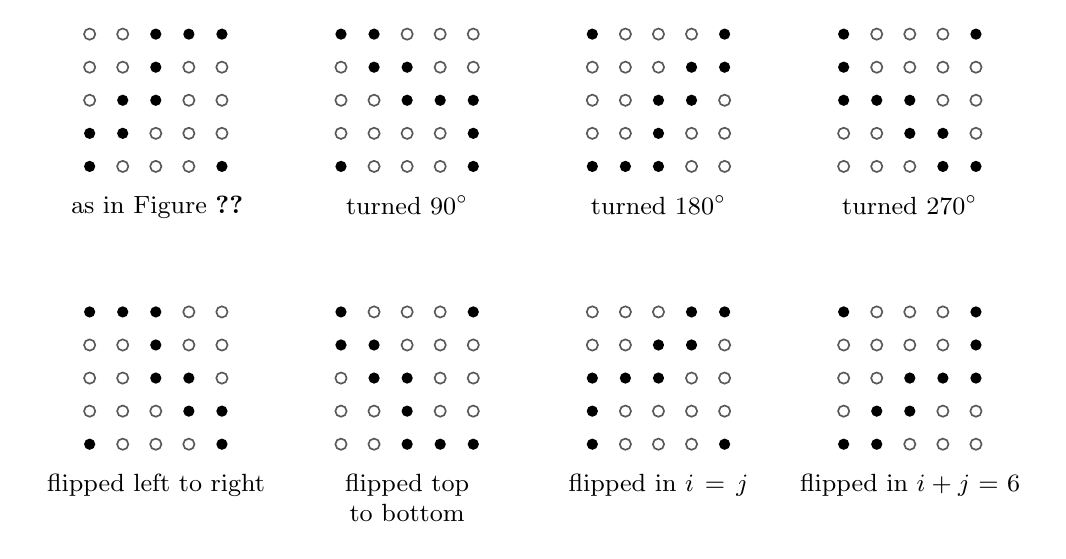
\begin{tikzpicture}[x=0.420cm,y=0.420cm,baseline=(current bounding box.north)]
  \begin{scope}[yshift=0.000cm]
  \filldraw[fill=white,draw=keptline,line width=0.6pt] (1.0,-1) circle (0.17);
  \filldraw[fill=white,draw=keptline,line width=0.6pt] (2.0,-1) circle (0.17);
  \fill[black] (3.0,-1) circle (0.17);
  \fill[black] (4.0,-1) circle (0.17);
  \fill[black] (5.0,-1) circle (0.17);
  \filldraw[fill=white,draw=keptline,line width=0.6pt] (1.0,-2) circle (0.17);
  \filldraw[fill=white,draw=keptline,line width=0.6pt] (2.0,-2) circle (0.17);
  \fill[black] (3.0,-2) circle (0.17);
  \filldraw[fill=white,draw=keptline,line width=0.6pt] (4.0,-2) circle (0.17);
  \filldraw[fill=white,draw=keptline,line width=0.6pt] (5.0,-2) circle (0.17);
  \filldraw[fill=white,draw=keptline,line width=0.6pt] (1.0,-3) circle (0.17);
  \fill[black] (2.0,-3) circle (0.17);
  \fill[black] (3.0,-3) circle (0.17);
  \filldraw[fill=white,draw=keptline,line width=0.6pt] (4.0,-3) circle (0.17);
  \filldraw[fill=white,draw=keptline,line width=0.6pt] (5.0,-3) circle (0.17);
  \fill[black] (1.0,-4) circle (0.17);
  \fill[black] (2.0,-4) circle (0.17);
  \filldraw[fill=white,draw=keptline,line width=0.6pt] (3.0,-4) circle (0.17);
  \filldraw[fill=white,draw=keptline,line width=0.6pt] (4.0,-4) circle (0.17);
  \filldraw[fill=white,draw=keptline,line width=0.6pt] (5.0,-4) circle (0.17);
  \fill[black] (1.0,-5) circle (0.17);
  \filldraw[fill=white,draw=keptline,line width=0.6pt] (2.0,-5) circle (0.17);
  \filldraw[fill=white,draw=keptline,line width=0.6pt] (3.0,-5) circle (0.17);
  \filldraw[fill=white,draw=keptline,line width=0.6pt] (4.0,-5) circle (0.17);
  \fill[black] (5.0,-5) circle (0.17);
  \node[capt,anchor=north,text width=3.02cm,align=center] at (3.0,-5.6) {as in Figure~\ref{fig:fivefive}};
  \end{scope}
  \begin{scope}[yshift=0.000cm]
  \fill[black] (8.6,-1) circle (0.17);
  \fill[black] (9.6,-1) circle (0.17);
  \filldraw[fill=white,draw=keptline,line width=0.6pt] (10.6,-1) circle (0.17);
  \filldraw[fill=white,draw=keptline,line width=0.6pt] (11.6,-1) circle (0.17);
  \filldraw[fill=white,draw=keptline,line width=0.6pt] (12.6,-1) circle (0.17);
  \filldraw[fill=white,draw=keptline,line width=0.6pt] (8.6,-2) circle (0.17);
  \fill[black] (9.6,-2) circle (0.17);
  \fill[black] (10.6,-2) circle (0.17);
  \filldraw[fill=white,draw=keptline,line width=0.6pt] (11.6,-2) circle (0.17);
  \filldraw[fill=white,draw=keptline,line width=0.6pt] (12.6,-2) circle (0.17);
  \filldraw[fill=white,draw=keptline,line width=0.6pt] (8.6,-3) circle (0.17);
  \filldraw[fill=white,draw=keptline,line width=0.6pt] (9.6,-3) circle (0.17);
  \fill[black] (10.6,-3) circle (0.17);
  \fill[black] (11.6,-3) circle (0.17);
  \fill[black] (12.6,-3) circle (0.17);
  \filldraw[fill=white,draw=keptline,line width=0.6pt] (8.6,-4) circle (0.17);
  \filldraw[fill=white,draw=keptline,line width=0.6pt] (9.6,-4) circle (0.17);
  \filldraw[fill=white,draw=keptline,line width=0.6pt] (10.6,-4) circle (0.17);
  \filldraw[fill=white,draw=keptline,line width=0.6pt] (11.6,-4) circle (0.17);
  \fill[black] (12.6,-4) circle (0.17);
  \fill[black] (8.6,-5) circle (0.17);
  \filldraw[fill=white,draw=keptline,line width=0.6pt] (9.6,-5) circle (0.17);
  \filldraw[fill=white,draw=keptline,line width=0.6pt] (10.6,-5) circle (0.17);
  \filldraw[fill=white,draw=keptline,line width=0.6pt] (11.6,-5) circle (0.17);
  \fill[black] (12.6,-5) circle (0.17);
  \node[capt,anchor=north,text width=3.02cm,align=center] at (10.6,-5.6) {turned $90^\circ$};
  \end{scope}
  \begin{scope}[yshift=0.000cm]
  \fill[black] (16.2,-1) circle (0.17);
  \filldraw[fill=white,draw=keptline,line width=0.6pt] (17.2,-1) circle (0.17);
  \filldraw[fill=white,draw=keptline,line width=0.6pt] (18.2,-1) circle (0.17);
  \filldraw[fill=white,draw=keptline,line width=0.6pt] (19.2,-1) circle (0.17);
  \fill[black] (20.2,-1) circle (0.17);
  \filldraw[fill=white,draw=keptline,line width=0.6pt] (16.2,-2) circle (0.17);
  \filldraw[fill=white,draw=keptline,line width=0.6pt] (17.2,-2) circle (0.17);
  \filldraw[fill=white,draw=keptline,line width=0.6pt] (18.2,-2) circle (0.17);
  \fill[black] (19.2,-2) circle (0.17);
  \fill[black] (20.2,-2) circle (0.17);
  \filldraw[fill=white,draw=keptline,line width=0.6pt] (16.2,-3) circle (0.17);
  \filldraw[fill=white,draw=keptline,line width=0.6pt] (17.2,-3) circle (0.17);
  \fill[black] (18.2,-3) circle (0.17);
  \fill[black] (19.2,-3) circle (0.17);
  \filldraw[fill=white,draw=keptline,line width=0.6pt] (20.2,-3) circle (0.17);
  \filldraw[fill=white,draw=keptline,line width=0.6pt] (16.2,-4) circle (0.17);
  \filldraw[fill=white,draw=keptline,line width=0.6pt] (17.2,-4) circle (0.17);
  \fill[black] (18.2,-4) circle (0.17);
  \filldraw[fill=white,draw=keptline,line width=0.6pt] (19.2,-4) circle (0.17);
  \filldraw[fill=white,draw=keptline,line width=0.6pt] (20.2,-4) circle (0.17);
  \fill[black] (16.2,-5) circle (0.17);
  \fill[black] (17.2,-5) circle (0.17);
  \fill[black] (18.2,-5) circle (0.17);
  \filldraw[fill=white,draw=keptline,line width=0.6pt] (19.2,-5) circle (0.17);
  \filldraw[fill=white,draw=keptline,line width=0.6pt] (20.2,-5) circle (0.17);
  \node[capt,anchor=north,text width=3.02cm,align=center] at (18.2,-5.6) {turned $180^\circ$};
  \end{scope}
  \begin{scope}[yshift=0.000cm]
  \fill[black] (23.799999999999997,-1) circle (0.17);
  \filldraw[fill=white,draw=keptline,line width=0.6pt] (24.799999999999997,-1) circle (0.17);
  \filldraw[fill=white,draw=keptline,line width=0.6pt] (25.799999999999997,-1) circle (0.17);
  \filldraw[fill=white,draw=keptline,line width=0.6pt] (26.799999999999997,-1) circle (0.17);
  \fill[black] (27.799999999999997,-1) circle (0.17);
  \fill[black] (23.799999999999997,-2) circle (0.17);
  \filldraw[fill=white,draw=keptline,line width=0.6pt] (24.799999999999997,-2) circle (0.17);
  \filldraw[fill=white,draw=keptline,line width=0.6pt] (25.799999999999997,-2) circle (0.17);
  \filldraw[fill=white,draw=keptline,line width=0.6pt] (26.799999999999997,-2) circle (0.17);
  \filldraw[fill=white,draw=keptline,line width=0.6pt] (27.799999999999997,-2) circle (0.17);
  \fill[black] (23.799999999999997,-3) circle (0.17);
  \fill[black] (24.799999999999997,-3) circle (0.17);
  \fill[black] (25.799999999999997,-3) circle (0.17);
  \filldraw[fill=white,draw=keptline,line width=0.6pt] (26.799999999999997,-3) circle (0.17);
  \filldraw[fill=white,draw=keptline,line width=0.6pt] (27.799999999999997,-3) circle (0.17);
  \filldraw[fill=white,draw=keptline,line width=0.6pt] (23.799999999999997,-4) circle (0.17);
  \filldraw[fill=white,draw=keptline,line width=0.6pt] (24.799999999999997,-4) circle (0.17);
  \fill[black] (25.799999999999997,-4) circle (0.17);
  \fill[black] (26.799999999999997,-4) circle (0.17);
  \filldraw[fill=white,draw=keptline,line width=0.6pt] (27.799999999999997,-4) circle (0.17);
  \filldraw[fill=white,draw=keptline,line width=0.6pt] (23.799999999999997,-5) circle (0.17);
  \filldraw[fill=white,draw=keptline,line width=0.6pt] (24.799999999999997,-5) circle (0.17);
  \filldraw[fill=white,draw=keptline,line width=0.6pt] (25.799999999999997,-5) circle (0.17);
  \fill[black] (26.799999999999997,-5) circle (0.17);
  \fill[black] (27.799999999999997,-5) circle (0.17);
  \node[capt,anchor=north,text width=3.02cm,align=center] at (25.799999999999997,-5.6) {turned $270^\circ$};
  \end{scope}
  \begin{scope}[yshift=-3.528cm]
  \fill[black] (1.0,-1) circle (0.17);
  \fill[black] (2.0,-1) circle (0.17);
  \fill[black] (3.0,-1) circle (0.17);
  \filldraw[fill=white,draw=keptline,line width=0.6pt] (4.0,-1) circle (0.17);
  \filldraw[fill=white,draw=keptline,line width=0.6pt] (5.0,-1) circle (0.17);
  \filldraw[fill=white,draw=keptline,line width=0.6pt] (1.0,-2) circle (0.17);
  \filldraw[fill=white,draw=keptline,line width=0.6pt] (2.0,-2) circle (0.17);
  \fill[black] (3.0,-2) circle (0.17);
  \filldraw[fill=white,draw=keptline,line width=0.6pt] (4.0,-2) circle (0.17);
  \filldraw[fill=white,draw=keptline,line width=0.6pt] (5.0,-2) circle (0.17);
  \filldraw[fill=white,draw=keptline,line width=0.6pt] (1.0,-3) circle (0.17);
  \filldraw[fill=white,draw=keptline,line width=0.6pt] (2.0,-3) circle (0.17);
  \fill[black] (3.0,-3) circle (0.17);
  \fill[black] (4.0,-3) circle (0.17);
  \filldraw[fill=white,draw=keptline,line width=0.6pt] (5.0,-3) circle (0.17);
  \filldraw[fill=white,draw=keptline,line width=0.6pt] (1.0,-4) circle (0.17);
  \filldraw[fill=white,draw=keptline,line width=0.6pt] (2.0,-4) circle (0.17);
  \filldraw[fill=white,draw=keptline,line width=0.6pt] (3.0,-4) circle (0.17);
  \fill[black] (4.0,-4) circle (0.17);
  \fill[black] (5.0,-4) circle (0.17);
  \fill[black] (1.0,-5) circle (0.17);
  \filldraw[fill=white,draw=keptline,line width=0.6pt] (2.0,-5) circle (0.17);
  \filldraw[fill=white,draw=keptline,line width=0.6pt] (3.0,-5) circle (0.17);
  \filldraw[fill=white,draw=keptline,line width=0.6pt] (4.0,-5) circle (0.17);
  \fill[black] (5.0,-5) circle (0.17);
  \node[capt,anchor=north,text width=3.02cm,align=center] at (3.0,-5.6) {flipped left to right};
  \end{scope}
  \begin{scope}[yshift=-3.528cm]
  \fill[black] (8.6,-1) circle (0.17);
  \filldraw[fill=white,draw=keptline,line width=0.6pt] (9.6,-1) circle (0.17);
  \filldraw[fill=white,draw=keptline,line width=0.6pt] (10.6,-1) circle (0.17);
  \filldraw[fill=white,draw=keptline,line width=0.6pt] (11.6,-1) circle (0.17);
  \fill[black] (12.6,-1) circle (0.17);
  \fill[black] (8.6,-2) circle (0.17);
  \fill[black] (9.6,-2) circle (0.17);
  \filldraw[fill=white,draw=keptline,line width=0.6pt] (10.6,-2) circle (0.17);
  \filldraw[fill=white,draw=keptline,line width=0.6pt] (11.6,-2) circle (0.17);
  \filldraw[fill=white,draw=keptline,line width=0.6pt] (12.6,-2) circle (0.17);
  \filldraw[fill=white,draw=keptline,line width=0.6pt] (8.6,-3) circle (0.17);
  \fill[black] (9.6,-3) circle (0.17);
  \fill[black] (10.6,-3) circle (0.17);
  \filldraw[fill=white,draw=keptline,line width=0.6pt] (11.6,-3) circle (0.17);
  \filldraw[fill=white,draw=keptline,line width=0.6pt] (12.6,-3) circle (0.17);
  \filldraw[fill=white,draw=keptline,line width=0.6pt] (8.6,-4) circle (0.17);
  \filldraw[fill=white,draw=keptline,line width=0.6pt] (9.6,-4) circle (0.17);
  \fill[black] (10.6,-4) circle (0.17);
  \filldraw[fill=white,draw=keptline,line width=0.6pt] (11.6,-4) circle (0.17);
  \filldraw[fill=white,draw=keptline,line width=0.6pt] (12.6,-4) circle (0.17);
  \filldraw[fill=white,draw=keptline,line width=0.6pt] (8.6,-5) circle (0.17);
  \filldraw[fill=white,draw=keptline,line width=0.6pt] (9.6,-5) circle (0.17);
  \fill[black] (10.6,-5) circle (0.17);
  \fill[black] (11.6,-5) circle (0.17);
  \fill[black] (12.6,-5) circle (0.17);
  \node[capt,anchor=north,text width=3.02cm,align=center] at (10.6,-5.6) {flipped top to bottom};
  \end{scope}
  \begin{scope}[yshift=-3.528cm]
  \filldraw[fill=white,draw=keptline,line width=0.6pt] (16.2,-1) circle (0.17);
  \filldraw[fill=white,draw=keptline,line width=0.6pt] (17.2,-1) circle (0.17);
  \filldraw[fill=white,draw=keptline,line width=0.6pt] (18.2,-1) circle (0.17);
  \fill[black] (19.2,-1) circle (0.17);
  \fill[black] (20.2,-1) circle (0.17);
  \filldraw[fill=white,draw=keptline,line width=0.6pt] (16.2,-2) circle (0.17);
  \filldraw[fill=white,draw=keptline,line width=0.6pt] (17.2,-2) circle (0.17);
  \fill[black] (18.2,-2) circle (0.17);
  \fill[black] (19.2,-2) circle (0.17);
  \filldraw[fill=white,draw=keptline,line width=0.6pt] (20.2,-2) circle (0.17);
  \fill[black] (16.2,-3) circle (0.17);
  \fill[black] (17.2,-3) circle (0.17);
  \fill[black] (18.2,-3) circle (0.17);
  \filldraw[fill=white,draw=keptline,line width=0.6pt] (19.2,-3) circle (0.17);
  \filldraw[fill=white,draw=keptline,line width=0.6pt] (20.2,-3) circle (0.17);
  \fill[black] (16.2,-4) circle (0.17);
  \filldraw[fill=white,draw=keptline,line width=0.6pt] (17.2,-4) circle (0.17);
  \filldraw[fill=white,draw=keptline,line width=0.6pt] (18.2,-4) circle (0.17);
  \filldraw[fill=white,draw=keptline,line width=0.6pt] (19.2,-4) circle (0.17);
  \filldraw[fill=white,draw=keptline,line width=0.6pt] (20.2,-4) circle (0.17);
  \fill[black] (16.2,-5) circle (0.17);
  \filldraw[fill=white,draw=keptline,line width=0.6pt] (17.2,-5) circle (0.17);
  \filldraw[fill=white,draw=keptline,line width=0.6pt] (18.2,-5) circle (0.17);
  \filldraw[fill=white,draw=keptline,line width=0.6pt] (19.2,-5) circle (0.17);
  \fill[black] (20.2,-5) circle (0.17);
  \node[capt,anchor=north,text width=3.02cm,align=center] at (18.2,-5.6) {flipped in $i=j$};
  \end{scope}
  \begin{scope}[yshift=-3.528cm]
  \fill[black] (23.799999999999997,-1) circle (0.17);
  \filldraw[fill=white,draw=keptline,line width=0.6pt] (24.799999999999997,-1) circle (0.17);
  \filldraw[fill=white,draw=keptline,line width=0.6pt] (25.799999999999997,-1) circle (0.17);
  \filldraw[fill=white,draw=keptline,line width=0.6pt] (26.799999999999997,-1) circle (0.17);
  \fill[black] (27.799999999999997,-1) circle (0.17);
  \filldraw[fill=white,draw=keptline,line width=0.6pt] (23.799999999999997,-2) circle (0.17);
  \filldraw[fill=white,draw=keptline,line width=0.6pt] (24.799999999999997,-2) circle (0.17);
  \filldraw[fill=white,draw=keptline,line width=0.6pt] (25.799999999999997,-2) circle (0.17);
  \filldraw[fill=white,draw=keptline,line width=0.6pt] (26.799999999999997,-2) circle (0.17);
  \fill[black] (27.799999999999997,-2) circle (0.17);
  \filldraw[fill=white,draw=keptline,line width=0.6pt] (23.799999999999997,-3) circle (0.17);
  \filldraw[fill=white,draw=keptline,line width=0.6pt] (24.799999999999997,-3) circle (0.17);
  \fill[black] (25.799999999999997,-3) circle (0.17);
  \fill[black] (26.799999999999997,-3) circle (0.17);
  \fill[black] (27.799999999999997,-3) circle (0.17);
  \filldraw[fill=white,draw=keptline,line width=0.6pt] (23.799999999999997,-4) circle (0.17);
  \fill[black] (24.799999999999997,-4) circle (0.17);
  \fill[black] (25.799999999999997,-4) circle (0.17);
  \filldraw[fill=white,draw=keptline,line width=0.6pt] (26.799999999999997,-4) circle (0.17);
  \filldraw[fill=white,draw=keptline,line width=0.6pt] (27.799999999999997,-4) circle (0.17);
  \fill[black] (23.799999999999997,-5) circle (0.17);
  \fill[black] (24.799999999999997,-5) circle (0.17);
  \filldraw[fill=white,draw=keptline,line width=0.6pt] (25.799999999999997,-5) circle (0.17);
  \filldraw[fill=white,draw=keptline,line width=0.6pt] (26.799999999999997,-5) circle (0.17);
  \filldraw[fill=white,draw=keptline,line width=0.6pt] (27.799999999999997,-5) circle (0.17);
  \node[capt,anchor=north,text width=3.02cm,align=center] at (25.799999999999997,-5.6) {flipped in $i+j=6$};
  \end{scope}
\end{tikzpicture}

\caption{The 8 maximum blackouts of the $5\times5$ grid. They are all different, so the optimum
is unique up to symmetry but has no symmetry of its own.}
\label{fig:orbit}
\end{figure}

\subsection{What the optimum looks like}

The optimum in Figure~\ref{fig:fivefive}(a) is a staircase of 9 points from the top-right corner
to the bottom-left corner, plus the corner $(5,5)$. The staircase alone has $9=n+m-1$ points and
its graph is a tree. The extra corner closes a cycle of length 8, the shortest the lemma allows.
The kept points form 2 blocks of 5 and 10 on either side of the staircase.

What about the other shape Lemma~\ref{lem:tenvertices} allows, a single 10-cycle? That means 2
black points in every row and every column, and there are 1,440 such sets. None of them is valid,
and the trouble always involves a tilted rectangle. Figure~\ref{fig:tencycle} shows one.

\begin{figure}[htbp]
\centering
% generated by make_figures.py; width about 3.6 cm
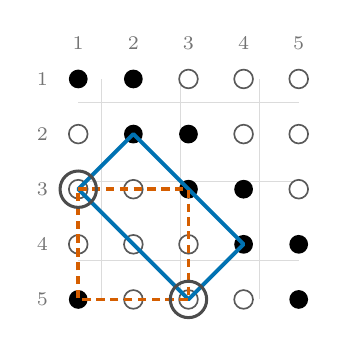
\begin{tikzpicture}[x=0.700cm,y=0.700cm,baseline=(current bounding box.north)]
  \draw[gridcol] (1,-1) grid (5,-5);
  \fill[black] (1,-1) circle (0.17);
  \fill[black] (2,-1) circle (0.17);
  \filldraw[fill=white,draw=keptline,line width=0.6pt] (3,-1) circle (0.17);
  \filldraw[fill=white,draw=keptline,line width=0.6pt] (4,-1) circle (0.17);
  \filldraw[fill=white,draw=keptline,line width=0.6pt] (5,-1) circle (0.17);
  \filldraw[fill=white,draw=keptline,line width=0.6pt] (1,-2) circle (0.17);
  \fill[black] (2,-2) circle (0.17);
  \fill[black] (3,-2) circle (0.17);
  \filldraw[fill=white,draw=keptline,line width=0.6pt] (4,-2) circle (0.17);
  \filldraw[fill=white,draw=keptline,line width=0.6pt] (5,-2) circle (0.17);
  \filldraw[fill=white,draw=keptline,line width=0.6pt] (1,-3) circle (0.17);
  \filldraw[fill=white,draw=keptline,line width=0.6pt] (2,-3) circle (0.17);
  \fill[black] (3,-3) circle (0.17);
  \fill[black] (4,-3) circle (0.17);
  \filldraw[fill=white,draw=keptline,line width=0.6pt] (5,-3) circle (0.17);
  \filldraw[fill=white,draw=keptline,line width=0.6pt] (1,-4) circle (0.17);
  \filldraw[fill=white,draw=keptline,line width=0.6pt] (2,-4) circle (0.17);
  \filldraw[fill=white,draw=keptline,line width=0.6pt] (3,-4) circle (0.17);
  \fill[black] (4,-4) circle (0.17);
  \fill[black] (5,-4) circle (0.17);
  \fill[black] (1,-5) circle (0.17);
  \filldraw[fill=white,draw=keptline,line width=0.6pt] (2,-5) circle (0.17);
  \filldraw[fill=white,draw=keptline,line width=0.6pt] (3,-5) circle (0.17);
  \filldraw[fill=white,draw=keptline,line width=0.6pt] (4,-5) circle (0.17);
  \fill[black] (5,-5) circle (0.17);
  \node[lab] at (1,-0.35) {1};
  \node[lab] at (2,-0.35) {2};
  \node[lab] at (3,-0.35) {3};
  \node[lab] at (4,-0.35) {4};
  \node[lab] at (5,-0.35) {5};
  \node[lab] at (0.35,-1) {1};
  \node[lab] at (0.35,-2) {2};
  \node[lab] at (0.35,-3) {3};
  \node[lab] at (0.35,-4) {4};
  \node[lab] at (0.35,-5) {5};
  \draw[draw=rectA,line width=1.4pt,line join=round] (1,-3) -- (2,-2) -- (4,-4) -- (3,-5) -- cycle;
  \draw[draw=rectB,line width=1.4pt,line join=round,dash pattern=on 3pt off 2pt] (1,-3) -- (3,-3) -- (3,-5) -- (1,-5) -- cycle;
  \draw[black!70,line width=1.1pt] (1,-3) circle (0.33);
  \draw[black!70,line width=1.1pt] (3,-5) circle (0.33);
\end{tikzpicture}

\caption{A 10-cycle blackout: 2 black points in every row and every column, and no short cycle.
The tilted rectangle (solid) and the axis-aligned one (dashed) both show only the ringed points
$(1,3)$ and $(3,5)$.}
\label{fig:tencycle}
\end{figure}

So the open question of a hand proof of uniqueness comes down to blackouts of 10 points whose
graph is connected with 1 cycle of length 8 or 10, and to the tilted rectangles on them.

%======================================================================
\section{Bigger grids}\label{sec:bigger}

What happens beyond 4 rows? The pattern on $5\times5$, a staircase from one corner to the
opposite corner plus 1 more point, keeps working.

\begin{figure}[htbp]
\centering
% generated by make_figures.py; width about 11.7 cm
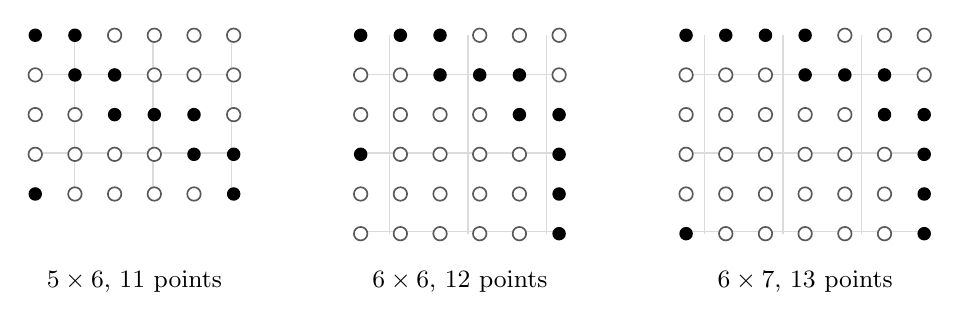
\begin{tikzpicture}[x=0.504cm,y=0.504cm,baseline=(current bounding box.north)]
  \draw[gridcol] (1,-1) grid (6,-5);
  \fill[black] (1,-1) circle (0.17);
  \fill[black] (2,-1) circle (0.17);
  \filldraw[fill=white,draw=keptline,line width=0.6pt] (3,-1) circle (0.17);
  \filldraw[fill=white,draw=keptline,line width=0.6pt] (4,-1) circle (0.17);
  \filldraw[fill=white,draw=keptline,line width=0.6pt] (5,-1) circle (0.17);
  \filldraw[fill=white,draw=keptline,line width=0.6pt] (6,-1) circle (0.17);
  \filldraw[fill=white,draw=keptline,line width=0.6pt] (1,-2) circle (0.17);
  \fill[black] (2,-2) circle (0.17);
  \fill[black] (3,-2) circle (0.17);
  \filldraw[fill=white,draw=keptline,line width=0.6pt] (4,-2) circle (0.17);
  \filldraw[fill=white,draw=keptline,line width=0.6pt] (5,-2) circle (0.17);
  \filldraw[fill=white,draw=keptline,line width=0.6pt] (6,-2) circle (0.17);
  \filldraw[fill=white,draw=keptline,line width=0.6pt] (1,-3) circle (0.17);
  \filldraw[fill=white,draw=keptline,line width=0.6pt] (2,-3) circle (0.17);
  \fill[black] (3,-3) circle (0.17);
  \fill[black] (4,-3) circle (0.17);
  \fill[black] (5,-3) circle (0.17);
  \filldraw[fill=white,draw=keptline,line width=0.6pt] (6,-3) circle (0.17);
  \filldraw[fill=white,draw=keptline,line width=0.6pt] (1,-4) circle (0.17);
  \filldraw[fill=white,draw=keptline,line width=0.6pt] (2,-4) circle (0.17);
  \filldraw[fill=white,draw=keptline,line width=0.6pt] (3,-4) circle (0.17);
  \filldraw[fill=white,draw=keptline,line width=0.6pt] (4,-4) circle (0.17);
  \fill[black] (5,-4) circle (0.17);
  \fill[black] (6,-4) circle (0.17);
  \fill[black] (1,-5) circle (0.17);
  \filldraw[fill=white,draw=keptline,line width=0.6pt] (2,-5) circle (0.17);
  \filldraw[fill=white,draw=keptline,line width=0.6pt] (3,-5) circle (0.17);
  \filldraw[fill=white,draw=keptline,line width=0.6pt] (4,-5) circle (0.17);
  \filldraw[fill=white,draw=keptline,line width=0.6pt] (5,-5) circle (0.17);
  \fill[black] (6,-5) circle (0.17);
  \node[capt,anchor=north] at (3.5,-6.7) {$5\times6$, 11 points};
  \draw[gridcol] (9.2,-1) grid (14.2,-6);
  \fill[black] (9.2,-1) circle (0.17);
  \fill[black] (10.2,-1) circle (0.17);
  \fill[black] (11.2,-1) circle (0.17);
  \filldraw[fill=white,draw=keptline,line width=0.6pt] (12.2,-1) circle (0.17);
  \filldraw[fill=white,draw=keptline,line width=0.6pt] (13.2,-1) circle (0.17);
  \filldraw[fill=white,draw=keptline,line width=0.6pt] (14.2,-1) circle (0.17);
  \filldraw[fill=white,draw=keptline,line width=0.6pt] (9.2,-2) circle (0.17);
  \filldraw[fill=white,draw=keptline,line width=0.6pt] (10.2,-2) circle (0.17);
  \fill[black] (11.2,-2) circle (0.17);
  \fill[black] (12.2,-2) circle (0.17);
  \fill[black] (13.2,-2) circle (0.17);
  \filldraw[fill=white,draw=keptline,line width=0.6pt] (14.2,-2) circle (0.17);
  \filldraw[fill=white,draw=keptline,line width=0.6pt] (9.2,-3) circle (0.17);
  \filldraw[fill=white,draw=keptline,line width=0.6pt] (10.2,-3) circle (0.17);
  \filldraw[fill=white,draw=keptline,line width=0.6pt] (11.2,-3) circle (0.17);
  \filldraw[fill=white,draw=keptline,line width=0.6pt] (12.2,-3) circle (0.17);
  \fill[black] (13.2,-3) circle (0.17);
  \fill[black] (14.2,-3) circle (0.17);
  \fill[black] (9.2,-4) circle (0.17);
  \filldraw[fill=white,draw=keptline,line width=0.6pt] (10.2,-4) circle (0.17);
  \filldraw[fill=white,draw=keptline,line width=0.6pt] (11.2,-4) circle (0.17);
  \filldraw[fill=white,draw=keptline,line width=0.6pt] (12.2,-4) circle (0.17);
  \filldraw[fill=white,draw=keptline,line width=0.6pt] (13.2,-4) circle (0.17);
  \fill[black] (14.2,-4) circle (0.17);
  \filldraw[fill=white,draw=keptline,line width=0.6pt] (9.2,-5) circle (0.17);
  \filldraw[fill=white,draw=keptline,line width=0.6pt] (10.2,-5) circle (0.17);
  \filldraw[fill=white,draw=keptline,line width=0.6pt] (11.2,-5) circle (0.17);
  \filldraw[fill=white,draw=keptline,line width=0.6pt] (12.2,-5) circle (0.17);
  \filldraw[fill=white,draw=keptline,line width=0.6pt] (13.2,-5) circle (0.17);
  \fill[black] (14.2,-5) circle (0.17);
  \filldraw[fill=white,draw=keptline,line width=0.6pt] (9.2,-6) circle (0.17);
  \filldraw[fill=white,draw=keptline,line width=0.6pt] (10.2,-6) circle (0.17);
  \filldraw[fill=white,draw=keptline,line width=0.6pt] (11.2,-6) circle (0.17);
  \filldraw[fill=white,draw=keptline,line width=0.6pt] (12.2,-6) circle (0.17);
  \filldraw[fill=white,draw=keptline,line width=0.6pt] (13.2,-6) circle (0.17);
  \fill[black] (14.2,-6) circle (0.17);
  \node[capt,anchor=north] at (11.7,-6.7) {$6\times6$, 12 points};
  \draw[gridcol] (17.4,-1) grid (23.4,-6);
  \fill[black] (17.4,-1) circle (0.17);
  \fill[black] (18.4,-1) circle (0.17);
  \fill[black] (19.4,-1) circle (0.17);
  \fill[black] (20.4,-1) circle (0.17);
  \filldraw[fill=white,draw=keptline,line width=0.6pt] (21.4,-1) circle (0.17);
  \filldraw[fill=white,draw=keptline,line width=0.6pt] (22.4,-1) circle (0.17);
  \filldraw[fill=white,draw=keptline,line width=0.6pt] (23.4,-1) circle (0.17);
  \filldraw[fill=white,draw=keptline,line width=0.6pt] (17.4,-2) circle (0.17);
  \filldraw[fill=white,draw=keptline,line width=0.6pt] (18.4,-2) circle (0.17);
  \filldraw[fill=white,draw=keptline,line width=0.6pt] (19.4,-2) circle (0.17);
  \fill[black] (20.4,-2) circle (0.17);
  \fill[black] (21.4,-2) circle (0.17);
  \fill[black] (22.4,-2) circle (0.17);
  \filldraw[fill=white,draw=keptline,line width=0.6pt] (23.4,-2) circle (0.17);
  \filldraw[fill=white,draw=keptline,line width=0.6pt] (17.4,-3) circle (0.17);
  \filldraw[fill=white,draw=keptline,line width=0.6pt] (18.4,-3) circle (0.17);
  \filldraw[fill=white,draw=keptline,line width=0.6pt] (19.4,-3) circle (0.17);
  \filldraw[fill=white,draw=keptline,line width=0.6pt] (20.4,-3) circle (0.17);
  \filldraw[fill=white,draw=keptline,line width=0.6pt] (21.4,-3) circle (0.17);
  \fill[black] (22.4,-3) circle (0.17);
  \fill[black] (23.4,-3) circle (0.17);
  \filldraw[fill=white,draw=keptline,line width=0.6pt] (17.4,-4) circle (0.17);
  \filldraw[fill=white,draw=keptline,line width=0.6pt] (18.4,-4) circle (0.17);
  \filldraw[fill=white,draw=keptline,line width=0.6pt] (19.4,-4) circle (0.17);
  \filldraw[fill=white,draw=keptline,line width=0.6pt] (20.4,-4) circle (0.17);
  \filldraw[fill=white,draw=keptline,line width=0.6pt] (21.4,-4) circle (0.17);
  \filldraw[fill=white,draw=keptline,line width=0.6pt] (22.4,-4) circle (0.17);
  \fill[black] (23.4,-4) circle (0.17);
  \filldraw[fill=white,draw=keptline,line width=0.6pt] (17.4,-5) circle (0.17);
  \filldraw[fill=white,draw=keptline,line width=0.6pt] (18.4,-5) circle (0.17);
  \filldraw[fill=white,draw=keptline,line width=0.6pt] (19.4,-5) circle (0.17);
  \filldraw[fill=white,draw=keptline,line width=0.6pt] (20.4,-5) circle (0.17);
  \filldraw[fill=white,draw=keptline,line width=0.6pt] (21.4,-5) circle (0.17);
  \filldraw[fill=white,draw=keptline,line width=0.6pt] (22.4,-5) circle (0.17);
  \fill[black] (23.4,-5) circle (0.17);
  \fill[black] (17.4,-6) circle (0.17);
  \filldraw[fill=white,draw=keptline,line width=0.6pt] (18.4,-6) circle (0.17);
  \filldraw[fill=white,draw=keptline,line width=0.6pt] (19.4,-6) circle (0.17);
  \filldraw[fill=white,draw=keptline,line width=0.6pt] (20.4,-6) circle (0.17);
  \filldraw[fill=white,draw=keptline,line width=0.6pt] (21.4,-6) circle (0.17);
  \filldraw[fill=white,draw=keptline,line width=0.6pt] (22.4,-6) circle (0.17);
  \fill[black] (23.4,-6) circle (0.17);
  \node[capt,anchor=north] at (20.4,-6.7) {$6\times7$, 13 points};
\end{tikzpicture}

\caption{Valid blackouts of $n+m$ points on $5\times6$, $6\times6$ and $6\times7$: a staircase
from one corner to the opposite corner, plus 1 more point.}
\label{fig:stairs}
\end{figure}

While building the game (\texttt{game/}), a search found a valid blackout of $n+m$ points of this
kind on every grid from $5\times5$ up to $10\times10$, and the game stores 1 for each size. The
script \texttt{verify\_narrow.py} rechecks all 21 of them with its own rectangle list, which shares
no code with the game, and they are all valid. So on every grid with both sides between 5 and 10,
\[
n+m\;\le\;\text{maximum blackout}\;\le\;\min\bigl(m+\lfloor n^2/4\rfloor,\;n+\lfloor m^2/4\rfloor\bigr).
\]
For $5\times5$ both ends meet only after Lemma~\ref{lem:tenvertices}. For $5\times6$, $5\times7$
and $6\times6$ the hitting set program found the value $n+m$ exactly. Everything we have seen
fits the following guess.

\begin{conjecture}[Excess-1]\label{conj:excess}
If $\min(n,m)\ge4$, the maximum blackout of the $n\times m$ grid is $n+m$, except for $4\times4$
and $4\times5$ (and their transposes), where it is $n+m-1$.
\end{conjecture}

The four-row case is now Theorem~\ref{thm:fourrow} with Corollary~\ref{cor:fourboundary}, and
$5\times5$ is Theorem~\ref{thm:fivefive}. The rest is open. Neither the row bound nor
Lemma~\ref{lem:tenvertices} (which needs $n+m\le10$) is strong enough there.

%======================================================================
\section{Computations}\label{sec:computations}

\subsection{The programs}

Three separate programs were used, and they agree wherever more than 1 of them can run.
\begin{itemize}[leftmargin=*,itemsep=1pt]
\item \emph{The hitting set program} (\texttt{solver/engine.py}) lists the rectangles, builds the
difference sets, prunes them as in Section~\ref{sec:pruning}, and finds the smallest hitting set
with an integer linear program: one 0--1 variable $x_v$ for each point, minimize $\sum_vx_v$,
subject to $\sum_{v\in D}x_v\ge1$ for every constraint $D$. The value is $nm$ minus the optimum.
To count the optima it then lists every kept set of the smallest size and checks it.
\item \emph{The brute force check} (\texttt{solver/brute.py}) uses no lemma at all. It finds
rectangles by testing every 4-point set with the diagonal test, and it checks each blackout
straight from the definition by computing all presentations and looking for a repeat. It is slow
on purpose and only feasible up to about 30 points.
\item \emph{The narrow-grid verifier} (\texttt{verify\_narrow.py}) checks the lemmas and
constructions of Sections~\ref{sec:graph} to~\ref{sec:bigger}: Lemma~\ref{lem:girth} on all
74,304 blackouts of 5 small grids, the list of tilted rectangles, the constructions at widths up
to 128, the finite four-row checks, the $5\times5$ search and the stored large blackouts. It uses
only the Python standard library and runs in about 20 seconds.
\end{itemize}

\subsection{The values}

\begin{center}\small
\begin{tabular}{lrrrrl}
\toprule
grid & rectangles & max blackout & kept & optima & checked by \\
\midrule
$2\times2$ & 1 & 4 & 0 & 1 & hand, program, brute force \\
$2\times3$ & 3 & 4 & 2 & 12 & hand, program, brute force \\
$2\times4$ & 6 & 5 & 3 & 32 & hand, program, brute force \\
$2\times5$ & 10 & 6 & 4 & 80 & program, brute force (predicted) \\
$2\times6$ & 15 & 7 & 5 & 192 & program, brute force \\
$2\times7$ & 21 & 8 & 6 & 448 & program, brute force \\
$3\times3$ & 10 & 5 & 4 & 53 & program, brute force \\
$3\times4$ & 20 & 6 & 6 & 224 & program, brute force \\
$3\times5$ & 33 & 7 & 8 & 892 & program, brute force \\
$3\times6$ & 49 & 8 & 10 & 3420 & program, brute force \\
$3\times7$ & 68 & 9 & 12 & 12704 & program, brute force \\
$3\times8$ & 90 & 10 & 14 & 45864 & program, brute force \\
$3\times9$ & 115 & 11 & 16 & 161992 & program, brute force \\
$3\times10$ & 143 & 12 & 18 & -- & program (value only) \\
$4\times4$ & 44 & 7 & 9 & 316 & program, brute force \\
$4\times5$ & 74 & 8 & 12 & 1810 & program, brute force \\
$4\times6$ & 110 & 10 & 14 & 26 & program, brute force \\
$4\times7$ & 152 & 11 & 17 & 292 & program, brute force \\
$4\times8$ & 200 & 12 & 20 & -- & program (value only) \\
$5\times5$ & 130 & 10 & 15 & 8 & program, brute force \\
$5\times6$ & 198 & 11 & 19 & -- & program (value only) \\
$5\times7$ & 276 & 12 & 23 & -- & program (value only) \\
$6\times6$ & 313 & 12 & 24 & -- & program (value only) \\
\bottomrule
\end{tabular}
\end{center}

Every value for 2, 3 and 4 rows and the value for $5\times5$ now also follow from proofs in these
notes. The values for $5\times6$, $5\times7$ and $6\times6$ rest on the program, with the lower
bound $n+m$ also confirmed by the stored blackouts of Section~\ref{sec:bigger}. The counts of
optima beyond 2 rows are only computed.

\begin{figure}[htbp]
\centering
% generated by make_figures.py; width about 8.4 cm
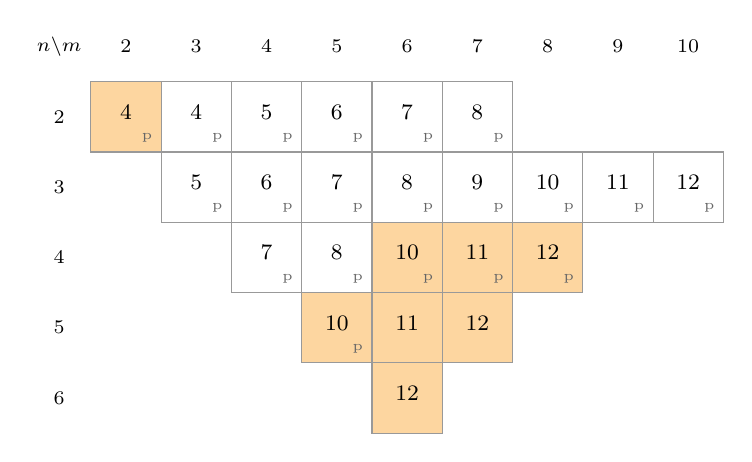
\begin{tikzpicture}[x=0.595cm,y=0.595cm,baseline=(current bounding box.north)]
  \filldraw[fill=white,draw=black!40] (0.75,-0.75) rectangle (2.25,0.75);
  \node[font=\footnotesize] at (1.5,0.1) {4};
  \node[font=\tiny,black!60] at (1.95,-0.45) {p};
  \filldraw[fill=white,draw=black!40] (2.25,-0.75) rectangle (3.75,0.75);
  \node[font=\footnotesize] at (3.0,0.1) {5};
  \node[font=\tiny,black!60] at (3.45,-0.45) {p};
  \filldraw[fill=white,draw=black!40] (3.75,-0.75) rectangle (5.25,0.75);
  \node[font=\footnotesize] at (4.5,0.1) {6};
  \node[font=\tiny,black!60] at (4.95,-0.45) {p};
  \filldraw[fill=white,draw=black!40] (5.25,-0.75) rectangle (6.75,0.75);
  \node[font=\footnotesize] at (6.0,0.1) {7};
  \node[font=\tiny,black!60] at (6.45,-0.45) {p};
  \filldraw[fill=white,draw=black!40] (6.75,-0.75) rectangle (8.25,0.75);
  \node[font=\footnotesize] at (7.5,0.1) {8};
  \node[font=\tiny,black!60] at (7.95,-0.45) {p};
  \filldraw[fill=excesscol,draw=black!40] (-0.75,-0.75) rectangle (0.75,0.75);
  \node[font=\footnotesize] at (0.0,0.1) {4};
  \node[font=\tiny,black!60] at (0.45,-0.45) {p};
  \filldraw[fill=white,draw=black!40] (0.75,-2.25) rectangle (2.25,-0.75);
  \node[font=\footnotesize] at (1.5,-1.4) {5};
  \node[font=\tiny,black!60] at (1.95,-1.95) {p};
  \filldraw[fill=white,draw=black!40] (2.25,-2.25) rectangle (3.75,-0.75);
  \node[font=\footnotesize] at (3.0,-1.4) {6};
  \node[font=\tiny,black!60] at (3.45,-1.95) {p};
  \filldraw[fill=white,draw=black!40] (3.75,-2.25) rectangle (5.25,-0.75);
  \node[font=\footnotesize] at (4.5,-1.4) {7};
  \node[font=\tiny,black!60] at (4.95,-1.95) {p};
  \filldraw[fill=white,draw=black!40] (5.25,-2.25) rectangle (6.75,-0.75);
  \node[font=\footnotesize] at (6.0,-1.4) {8};
  \node[font=\tiny,black!60] at (6.45,-1.95) {p};
  \filldraw[fill=white,draw=black!40] (6.75,-2.25) rectangle (8.25,-0.75);
  \node[font=\footnotesize] at (7.5,-1.4) {9};
  \node[font=\tiny,black!60] at (7.95,-1.95) {p};
  \filldraw[fill=white,draw=black!40] (8.25,-2.25) rectangle (9.75,-0.75);
  \node[font=\footnotesize] at (9.0,-1.4) {10};
  \node[font=\tiny,black!60] at (9.45,-1.95) {p};
  \filldraw[fill=white,draw=black!40] (9.75,-2.25) rectangle (11.25,-0.75);
  \node[font=\footnotesize] at (10.5,-1.4) {11};
  \node[font=\tiny,black!60] at (10.95,-1.95) {p};
  \filldraw[fill=white,draw=black!40] (11.25,-2.25) rectangle (12.75,-0.75);
  \node[font=\footnotesize] at (12.0,-1.4) {12};
  \node[font=\tiny,black!60] at (12.45,-1.95) {p};
  \filldraw[fill=white,draw=black!40] (2.25,-3.75) rectangle (3.75,-2.25);
  \node[font=\footnotesize] at (3.0,-2.9) {7};
  \node[font=\tiny,black!60] at (3.45,-3.45) {p};
  \filldraw[fill=white,draw=black!40] (3.75,-3.75) rectangle (5.25,-2.25);
  \node[font=\footnotesize] at (4.5,-2.9) {8};
  \node[font=\tiny,black!60] at (4.95,-3.45) {p};
  \filldraw[fill=excesscol,draw=black!40] (5.25,-3.75) rectangle (6.75,-2.25);
  \node[font=\footnotesize] at (6.0,-2.9) {10};
  \node[font=\tiny,black!60] at (6.45,-3.45) {p};
  \filldraw[fill=excesscol,draw=black!40] (6.75,-3.75) rectangle (8.25,-2.25);
  \node[font=\footnotesize] at (7.5,-2.9) {11};
  \node[font=\tiny,black!60] at (7.95,-3.45) {p};
  \filldraw[fill=excesscol,draw=black!40] (8.25,-3.75) rectangle (9.75,-2.25);
  \node[font=\footnotesize] at (9.0,-2.9) {12};
  \node[font=\tiny,black!60] at (9.45,-3.45) {p};
  \filldraw[fill=excesscol,draw=black!40] (3.75,-5.25) rectangle (5.25,-3.75);
  \node[font=\footnotesize] at (4.5,-4.4) {10};
  \node[font=\tiny,black!60] at (4.95,-4.95) {p};
  \filldraw[fill=excesscol,draw=black!40] (5.25,-5.25) rectangle (6.75,-3.75);
  \node[font=\footnotesize] at (6.0,-4.4) {11};
  \filldraw[fill=excesscol,draw=black!40] (6.75,-5.25) rectangle (8.25,-3.75);
  \node[font=\footnotesize] at (7.5,-4.4) {12};
  \filldraw[fill=excesscol,draw=black!40] (5.25,-6.75) rectangle (6.75,-5.25);
  \node[font=\footnotesize] at (6.0,-5.9) {12};
  \node[tiny] at (0.0,1.5) {$2$};
  \node[tiny] at (1.5,1.5) {$3$};
  \node[tiny] at (3.0,1.5) {$4$};
  \node[tiny] at (4.5,1.5) {$5$};
  \node[tiny] at (6.0,1.5) {$6$};
  \node[tiny] at (7.5,1.5) {$7$};
  \node[tiny] at (9.0,1.5) {$8$};
  \node[tiny] at (10.5,1.5) {$9$};
  \node[tiny] at (12.0,1.5) {$10$};
  \node[tiny] at (-1.4249999999999998,0.0) {$2$};
  \node[tiny] at (-1.4249999999999998,-1.5) {$3$};
  \node[tiny] at (-1.4249999999999998,-3.0) {$4$};
  \node[tiny] at (-1.4249999999999998,-4.5) {$5$};
  \node[tiny] at (-1.4249999999999998,-6.0) {$6$};
  \node[tiny] at (-1.4249999999999998,1.5) {$n\backslash m$};
\end{tikzpicture}

\caption{The maximum blackout of each computed $n\times m$ grid. Shaded cells beat $n+m-1$ by
exactly 1, white cells equal it. A small ``p'' marks a value that is proved. ($2\times2$ is the
trivial grid with only 1 rectangle.)}
\label{fig:excess}
\end{figure}

\subsection{Predictions that failed}

Before most computations a prediction was written in the ledger (\texttt{data/ledger.md}), so
that the computation could prove it wrong. Several did go wrong.

\begin{center}\small
\begin{tabular}{lll}
\toprule
guess & where it failed & what happened \\
\midrule
kept $=(n-1)(m-1)$, so blackout $n+m-1$ & $5\times5$ & 10 instead of 9 \\
blackout $=n+m-1+[\,n+m\ge10\,]$ & $3\times7$ & 9 instead of 10 \\
blackout $=n+m-1+[\,nm\ge24\,]$ & $3\times8$ & 10 instead of 11 \\
kept on 4 rows $=\lceil5m/2\rceil-1$ & $4\times8$ & 12 instead of 13 \\
\bottomrule
\end{tabular}
\end{center}

The first guess fit all 8 values computed before $5\times5$. The $5\times5$ grid broke it, and it
also has only 8 optima against 1,810 on $4\times5$, so something changes there. The next 2 guesses
tried to say when the extra point appears, by the sum or by the area of the grid, and 3 rows
killed both: 3 rows never get the extra point. The four-row formula fit 4 values and died on the
fifth. What survived is what is now proved: $m+1$, $m+2$ and $m+4$ on 2, 3 and 4 rows, and the
Excess-1 conjecture beyond.

%======================================================================
\section{Open questions}\label{sec:open}

\begin{enumerate}[leftmargin=*,itemsep=2pt]
\item Prove Conjecture~\ref{conj:excess} when both sides are at least 5. The lower bound $n+m$ is
known up to $10\times10$ by computer; a general construction and a matching upper bound are both
missing.
\item Count the optima beyond 2 rows. Why does the number collapse to 26 on $4\times6$, when its
neighbours have hundreds or thousands?
\item Prove that the $5\times5$ optimum is unique up to symmetry without a computer.
Theorem~\ref{thm:fivefive} reduces this to blackouts whose graph is connected with 1 cycle of
length 8 or 10.
\item Does the excess over $n+m-1$ ever reach 2? The next grids to try are $5\times8$ and
$6\times7$, where the ledger predicts 13.
\item The row--column graph turns the axis-aligned part into a question about bipartite graphs
with no 4- or 6-cycle. How does this compare with the literature on test covers and on extremal
graphs of large girth?
\end{enumerate}

\begin{thebibliography}{9}
\bibitem{kagey} P. Kagey, Problem 001, Open Problem Collection,
\url{https://peterkagey.com/problems/001/} (accessed August 2026).
\bibitem{oeisA085582} OEIS Foundation, Sequence A085582: number of rectangles (orthogonal or not)
with corners on an $n\times n$ grid of points, \url{https://oeis.org/A085582}.
\bibitem{oeisA289832} OEIS Foundation, Sequence A289832: number of rectangles with corners on an
$n\times k$ grid of points, \url{https://oeis.org/A289832}. Here $T(n,k)$ counts rectangles on an
$(n+1)\times(k+1)$ grid of points, so our $r\times c$ grid is $T(c-1,r-1)$; for example our
$3\times7$ count is $T(6,2)=68$.
\end{thebibliography}

\end{document}
